% \iffalse meta-comment
%
% powerdot class by Hendri Adriaens and Christopher Ellison.
%
% Extract package files and create documentation:
%    Find powerdot.dtx
%    Remove \OnlyDescription from the file
%    latex powerdot.dtx
%    latex powerdot.dtx
%    bibtex powerdot
%    makeindex -s gglo.ist -o powerdot.gls powerdot.glo
%    makeindex -s gind.ist -o powerdot.ind powerdot.idx
%    latex powerdot.dtx
%    latex powerdot.dtx
%
% To finish the installation you have to move the following
% files into a directory searched by LaTeX:
%    powerdot.cls
%    powerdot-default.sty
%    powerdot-default.ps
%    powerdot-tycja.sty
%    powerdot-ikeda.sty
%    powerdot-fyma.sty
%    powerdot-simple.sty
%
%% ----------------------------------------------------------
%% Copyright (C) 2005 Hendri Adriaens and Christopher Ellison
%% ----------------------------------------------------------
%%
%% This work may be distributed and/or modified under the
%% conditions of the LaTeX Project Public License, either version 1.3
%% of this license or (at your option) any later version.
%% The latest version of this license is in
%%   http://www.latex-project.org/lppl.txt
%% and version 1.3 or later is part of all distributions of LaTeX
%% version 2003/12/01 or later.
%%
%% This work has the LPPL maintenance status "maintained".
%%
%% This Current Maintainer of this work is Christopher Ellison.
%%
%% This work consists of the file powerdot.dtx and derived files
%% powerdot.cls, powerdot-default.sty, powerdot-tycja.sty,
%% powerdot-ikeda.sty, powerdot-fyma.sty, powerdot-simple.sty,
%% powerdot-ciment.sty, powerdot-styletest.tex, powerdot-example1.tex
%% and powerdot-example2.tex.
%%
%% The following files constitute the powerdot bundle and must be
%% distributed as a whole: readme, powerdot.pdf, powerdot.dtx,
%% powerdot.cls, powerdot-default.sty, powerdot-default.ps,
%% powerdot-tycja.sty, powerdot-ikeda.sty, powerdot-fyma.sty,
%% powerdot-simple.sty, powerdot-ciment.sty, powerdot-example1.tex
%% and powerdot-example2.tex.
%%
% \fi
%
% \iffalse
%<*batchfile>
\begingroup
\input docstrip
\keepsilent
\preamble
\endpreamble
\askforoverwritefalse
\generate{
  \file{powerdot.cls}{\from{powerdot.dtx}{powerdot}}
  \file{powerdot-default.sty}{\from{powerdot.dtx}{pddefault}}
  \file{powerdot-tycja.sty}{\from{powerdot.dtx}{pdtycja}}
  \file{powerdot-ikeda.sty}{\from{powerdot.dtx}{pdikeda}}
  \file{powerdot-fyma.sty}{\from{powerdot.dtx}{pdfyma}}
  \file{powerdot-simple.sty}{\from{powerdot.dtx}{pdsimple}}
  \file{powerdot-ciment.sty}{\from{powerdot.dtx}{pdciment}}
  \file{powerdot-styletest.tex}{\from{powerdot.dtx}{pdstyletest}}
  \file{powerdot-example1.tex}{\from{powerdot.dtx}{pdexample1}}
  \file{powerdot-example2.tex}{\from{powerdot.dtx}{pdexample2}}
  \file{pdpream.ble}{\from{powerdot.dtx}{preamble}}
  \file{powerdot.bib}{\from{powerdot.dtx}{bib}}
}
\endgroup
%</batchfile>
%<*driver>
\documentclass[a4paper]{ltxdoc}
\input{pdpream.ble}
\OnlyDescription
%\EnableCrossrefs
\def\fileversion{v1.0}
\def\filedate{2005/09/04}
\begin{document}
\DocInput{powerdot.dtx}
\let\Section\section\def\section*#1{\Section*{#1}\addcontentsline{toc}{section}{#1}}
\bibliographystyle{plain}
\bibliography{powerdot}
\section*{Acknowledgements}
The authors are grateful to Darren Dale and Herbert Vo\ss\ for
testing the class and its output. Further, we like to thank all
style contributors (see section~\ref{sec:styles}) and the testers of
the first beta releases.
\PrintChangesX\PrintIndexX
\end{document}
%</driver>
% \fi
%
% \changes{v1.0}{2005/09/04}{Initial release}
%
% \CheckSum{2310}
%
% \CharacterTable
%  {Upper-case    \A\B\C\D\E\F\G\H\I\J\K\L\M\N\O\P\Q\R\S\T\U\V\W\X\Y\Z
%   Lower-case    \a\b\c\d\e\f\g\h\i\j\k\l\m\n\o\p\q\r\s\t\u\v\w\x\y\z
%   Digits        \0\1\2\3\4\5\6\7\8\9
%   Exclamation   \!     Double quote  \"     Hash (number) \#
%   Dollar        \$     Percent       \%     Ampersand     \&
%   Acute accent  \'     Left paren    \(     Right paren   \)
%   Asterisk      \*     Plus          \+     Comma         \,
%   Minus         \-     Point         \.     Solidus       \/
%   Colon         \:     Semicolon     \;     Less than     \<
%   Equals        \=     Greater than  \>     Question mark \?
%   Commercial at \@     Left bracket  \[     Backslash     \\
%   Right bracket \]     Circumflex    \^     Underscore    \_
%   Grave accent  \`     Left brace    \{     Vertical bar  \|
%   Right brace   \}     Tilde         \~}
%
%\title{\vspace*{-2cm}\mktitledecor The \pf{powerdot} class
%\thanks{This class can be downloaded from the CTAN mirrors:
%\texttt{/macros/latex/contrib/powerdot}. See \texttt{powerdot.dtx} for
%information on installing \pf{powerdot} into your \LaTeX\
%distribution and for the license of this class.}}
%\author{Hendri Adriaens\and Christopher Ellison}
%\date{\fileversion\ (\filedate)}
%\maketitle
%
%\begin{abstract}\noindent
%\pf{powerdot} is a presentation class for \LaTeX\ that allows for
%the quick and easy development of professional presentations. It
%comes with many tools that enhance presentations and aid the
%presenter. Examples are automatic overlays, personal notes and a
%handout mode. To view a presentation, DVI, PS or PDF output can be
%used. A powerful template system is available to easily develop new
%styles.
%\end{abstract}
%
%\begin{multicols}{2}
%[\section*{Contents}
%\setlength{\columnseprule}{.4pt}
%\setlength{\columnsep}{18pt}]
%\tableofcontents
%\end{multicols}
%
%\newpage
%\section{Introduction}\label{sec:intro}
%This class gives you the possibility to easily create professionally
%looking slides. The class is designed to make the development of
%presentations as simple as possible so that you can concentrate on
%the actual content instead of keeping yourself busy with technical
%details. Of course, some knowledge of \LaTeX\ is still required
%though.
%
%This class builds on and extends the \pf{prosper} class
%\cite{prosper} and the \pf{HA-prosper} package \cite{HA-prosper}.
%The \pf{HA-prosper} package was initially intended to extend
%\pf{prosper} and correct some bugs and problems of that class. As
%developments on that package progressed, it was found that
%unfortunately, not all of the problems could be overcome with the
%package. That discovery was the start of a new project set up to
%make a new class to replace the \pf{prosper} plus \pf{HA-prosper}
%combination. You're currently reading the result of that project.
%
%The remainder of this section will be devoted to giving a feel of
%what the \pf{powerdot} presentation source looks like and giving an
%overview of this documentation.
%
%The document structure of a presentation is always the same. You can
%find it in the example below.
%
%\begin{example}
% \documentclass[<class options>]{powerdot}
% \pdsetup{<presentation options>}
% \begin{document}
%   \begin{slide}{a slide}
%     Contents of the slide.
%   \end{slide}
%   \section{first section}
%   \begin{slide}[<slide options>]{another slide}
%     Contents of the slide.
%   \end{slide}
%   \begin{note}{personal note}
%     The note.
%   \end{note}
% \end{document}
%\end{example}
%
%There are several elements that define the document structure. First
%of all, the class accepts some class options that control the output
%of the class, for instance, paper type and style. These class
%options will be discussed in section~\ref{sec:classopts}. Then there
%are presentation specific options which control some of the elements
%of the presentation globally, for instance, the footers. These will
%be discussed in section~\ref{sec:pdsetup}.
%
%Once the setup has been decided on, you can use the slide
%environment to produce slides (see section~\ref{sec:slides}) and the
%note environment to produce notes that go with the slides (see
%section~\ref{sec:notes}). You can use overlays to display material
%in steps. This is described in section~\ref{sec:overlays}. The
%|\section| command provides a way to structure your presentation.
%This is discussed in section~\ref{sec:structure}.
%Section~\ref{sec:styles} will show an overview of the styles that
%come with this class and the characteristics of each style.
%Section~\ref{sec:compiling} will tell you more about how to produce
%output. This section contains important information on required
%packages.
%
%Section~\ref{sec:writestyle} is mostly interesting for people that
%want to develop their own style for this class or want to modify
%an existing style. This documentation concludes with a section
%devoted to questions (section~\ref{sec:questions}), like `Where can
%I find examples?'. It also tells you where to turn to in case your
%questions are still not solved.
%
%\section{Setting up the presentation}\label{sec:setup}
%This section will describe all options that are available to control
%the output of the presentation and the looks of it.
%
%\subsection{Document class options}\label{sec:classopts} We will
%start with the class options that are typed in the |\documentclass|
%command as a comma-separated list. For each option, the default
%value will be mentioned in the description. This is the value that
%will be used if you decide to not give a value to the option or not
%use the option at all.
%
%\DescribeOption{mode}
%This options controls the kind of output that we want to produce.
%The default value is |present|.
%\begin{description}
%\item\option{mode=present}\\
%This mode is used when you want to create the actual presentation. It
%will enable overlays and transition effects. You can read more about
%overlays in section~\ref{sec:overlays}.
%\item\option{mode=print}\\
%This mode can be used when printing the slides including their visual
%markup, but without any overlay or transition effects.
%\item\option{mode=handout}\\
%This mode will produce a black and white overview of your slides that
%can be used to make personal notes on, for distribution to students,
%a personal guide during your talk, etcetera.
%\begin{description}
%\item\option{nopagebreaks}\\
%By default, the handout mode produces a document with two slides per
%page. If you want to fit more slides on a page, specify this option
%in the |\documentclass| command and \pf{powerdot} will let \LaTeX\
%decide on the places to insert a page break, namely when a page is
%full.
%\end{description}
%\end{description}
%
%\DescribeOption{paper} This option has three possible values. The default
%value is |screen|.
%\begin{description}
%\item\option{paper=screen}\\
%This is a special format with screen optimized ratio (4/3). The
%actual page dimensions will be 8.25 inch by 11 inch. This paper format
%is not available for print or handout mode. In these modes, \pf{powerdot}
%will switch to a4 paper and put a warning that it did this in the
%log file of your presentation.
%\item\option{paper=a4paper}\\
%A4 paper will be used for the presentation or handout.
%\item\option{paper=letterpaper}\\
%Letter size paper will be used.
%\end{description}
%Some important information with respect to paper size, compiling and
%viewing presentations is available in section~\ref{sec:compiling}.
%
%\DescribeOption{orient} This controls the orientation of the
%presentation. The default value is |landscape|.
%\begin{description}
%\item\option{orient=landscape}\\
%The presentation will be in landscape format. This value is not
%available in handout mode. In that mode, \pf{powerdot} will switch
%to portrait orientation and will warn you about this in the log
%file.
%\item\option{orient=portrait}\\ This produces slides in portrait
%format. Notice that not all styles support portrait orientation. Please
%refer to section~\ref{sec:styles} for information about which styles
%do support the portrait orientation.
%\end{description}
%
%\DescribeOption{display} This controls the production of slides and
%notes. The default value is |slides|.
%\begin{description}
%\item\option{display=slides}\\
%This will only typeset the slides in your presentation.
%\item\option{display=slidesnotes}\\
%This will typeset both the slides and the notes in your
%presentation. See also section~\ref{sec:notes} for more information
%about notes.
%\item\option{display=notes}\\ This will typeset the notes only. To
%be able to typeset the slide numbers of the notes correctly, one should
%first run the presentation in slidesnotes mode once.
%\end{description}
%
%Here are some more options to control the output.
%\begin{description}
%\item\DescribeOption{size}\option{size}\\
%This is the size of the normal text font in points. Possible values
%are 8, 9, 10, 11, 12, 14, 17, 20 and the default value is
%11.\footnote{Note that sizes other than 10, 11 and 12 are
%non-standard and it is assumed that you have the \pf{extsizes}
%bundle \cite{extsizes} installed, which provides these sizes.}
%\item\DescribeOption{style}\option{style}\\
%This controls the style to be loaded for the presentation. By
%default, the \pf{default} style will be loaded. For more styles, see
%section~\ref{sec:styles}.
%\item\DescribeOption{fleqn}\option{fleqn}\\
%This option makes equations flushed left. It does the same as the
%equally named option for the article class.
%\item\DescribeOption{leqno}\option{leqno}\\
%Put equation numbers at the left. Also the same as in the article
%class.
%\item\DescribeOption{nopsheader}\option{nopsheader}\\
%By default, \pf{powerdot} will write a postscript command to the ps
%file to make sure that post processors like ps2pdf know which paper
%to use without the need to specify it on the command line. See also
%section~\ref{sec:compiling}. If you experience problems with post
%processing or printing or you want to specify the paper size in the
%post processing steps yourself, use this option.
%\item\DescribeOption{hlentries}\option{hlentries}\\
%This highlights table of contents entries when the entry matches
%with the current slide and is |true| by default. See also
%section~\ref{sec:structure}. If you don't want highlighting of table
%of contents entries (for instance in print mode), use
%|hlentries=false|.
%\item\DescribeOption{hlsections}\option{hlsections}\\
%This highlights table of contents sections when the section matches
%with the current section in the presentation and is |false| by
%default. See also section~\ref{sec:structure}. Specifying this
%option turns highlighting of sections on. This could be useful when
%you are using a style that implements a split table of contents.
%\item\DescribeOption{blackslide}\option{blackslide}\\
%This option inserts a black slide in the presentation on page 1 and
%will automatically advance to page 2 when opening the presentation
%in a PDF viewer like Acrobat (Reader). The black slide has an
%embedded target called |blackslide| and you can make a clickable
%link to this slide by using
%\begin{example}
% \hyperlink{blackslide}{Click here to go to the black slide}
%\end{example}
%When you click anywhere in the black slide, you will go back to the
%originating slide. This option can be used to temporarily pause a
%presentation, for instance, to do a proof on the black board.
%\end{description}
%
%Here is an example of a |\documentclass| command.
%\begin{example}
% \documentclass[
%   size=12,
%   paper=screen,
%   mode=present,
%   display=slidesnotes,
%   style=tycja,
%   nopagebreaks,
%   blackslide,
%   fleqn
% ]{powerdot}
%\end{example}
%This example sets up a presentation in \pf{tycja} style, with a black
%slide, normal size 12 points and flushed left equations.
%\begin{example}
% \documentclass[
%   size=12,
%   paper=letterpaper,
%   mode=handout,
%   display=slidesnotes,
%   style=tycja,
%   nopagebreaks,
%   blackslide,
%   fleqn
% ]{powerdot}
%\end{example}
%Changing the |paper| and |mode| options, now produces a handout with
%possibly more than two slides per page due to the |nopagebreaks|
%option.
%
%\subsection{Setup options}\label{sec:pdsetup}
%\DescribeMacro{\pdsetup}
%There are several extra options that can help customizing your
%presentation. These options are not available via the
%|\documentclass| command. This has a technical reason.\footnote{The
%interested reader is referred to the section about the \pf{xkvltxp}
%package in the \pf{xkeyval} package documentation \cite{xkeyval}.}
%The options can be accessed via the |\pdsetup| command, which can
%only be used in the preamble of your presentation. The command takes
%one argument, which should contain a comma-separated list of
%options. The available options are described below.
%
%\begin{description}
%\item\DescribeOption{lf}\option{lf}\\
%This determines the content of the left footer. By default, this is
%empty.
%\item\DescribeOption{rf}\option{rf}\\
%This determines the content of the right footer. By default, this is
%empty.
%\item\DescribeOption{theslide}\option{theslide}\\
%This option controls how the slide number appears on the slide. By
%default this has the value |\arabic{slide}~/~\pageref*{lastslide}|,
%which could appear like |5/22|. Notice that the |\arabic{slide}|
%typesets the number of the current slide and that
%|\pageref*{lastslide}| typesets the number of the last
%slide.\footnote{We use the starred version of \cs{pageref} which is
%defined by \pf{hyperref} and does not create a link to the page that
%it is referring to.}
%\item\DescribeOption{thenote}\option{thenote}\\
%This is similar to the |theslide| option, but typesets the slide
%numbers of notes. The default value is
%|note~\arabic{note}~of~slide~\arabic{slide}| and |\arabic{note}|
%here typesets the number of the current note that goes with the
%current slide. This could appear like |note 2 of slide 7|.
%\item\DescribeOption{trans}\option{trans}\\
%This option sets the default transition effect to be used in the
%presentation. These transition effects only work after compiling the
%presentation to PDF format. See also section~\ref{sec:compiling}.
%The following transition effects are supported: |Split|, |Blinds|,
%|Box|, |Wipe|, |Dissolve|, |Glitter| and |Replace|. When you are using
%a viewer that understands PDF 1.5, you can also use |Fly|, |Push|,
%|Cover|, |Uncover| or |Fade|. It is important to notice that most
%viewers are case sensitive, so, for instance, |box| will not work.
%
%The default effect is |Replace| which just replaces one slide with
%another when browsing the slides. Note that some PDF viewers (like
%Acrobat Reader 5 and higher) only produce the transition effect in
%full screen mode. If you want to use a custom transition effect that
%is not listed in the list above (for instance, a wipe effect with a
%custom wipe direction), then that is possible. However,
%\pf{powerdot} will put a warning in your log file that the effect
%that you have chosen, might not work in the PDF viewer. Here is an
%example that does work.
%\begin{example}
% trans=Wipe /Di 0
%\end{example}
%In Acrobat (Reader), this wipes from left to right instead of the
%default top to bottom. For more information, see a PDF Reference
%Manual.
%\item\DescribeOption{counters}\option{counters}\\
%The |counters| option lists counters that you might want to protect
%on overlays. As material on overlays (see
%section~\ref{sec:overlays}) is processed multiple times, also
%\LaTeX\ counters, like the |equation| counter, might be increased
%too often. To avoid that your equations get different numbers on
%every overlay, use this option. The |equation|, |table|, |figure|,
%|footnote| and |mpfootnote| counters are already protected for you.
%If you use extra counters, for instance for theorems, list them in
%this option. Example:
%\begin{example}
% counters={theorem,lemma}
%\end{example}
%\item\DescribeOption{list}\option{list}\\
%This option takes a list of options that will be passed on to the
%\pf{enumitem} package that controls the layout of lists created by
%the |enumerate| and |itemize| environments. Example:
%\begin{example}
% list={labelsep=1em,leftmargin=*,itemsep=0pt,topsep=5pt,parsep=0pt}
%\end{example}
%See for more information on controlling the layout of lists the
%\pf{enumitem} package \cite{enumitem}.
%\item\DescribeOption{enumerate}\option{enumerate}\\
%As the |list| option, but only control |enumerate| environments.
%\item\DescribeOption{itemize}\option{itemize}\\
%As the |list| option, but only control |itemize| environments.
%\end{description}
%
%Here is an example of a |\pdsetup| command that one could use to set up
%the presentation.
%\begin{example}
% \pdsetup{
%   lf=My first presentation,
%   rf=For some conference,
%   trans=Wipe,
%   theslide=\arabic{slide}
% }
%\end{example}
%This sets the left and right footers and will initialize the
%transition effect to |Wipe|. Further, slide numbers will not include
%the number of the last slide, but only the number of the current
%slide.
%
%A small note is necessary with respect to the appearance of footers.
%The slide number (controlled by the |theslide| option) will be added
%to a footer. Most styles add it too the right footer. If both the
%footer and the slide number are non empty, |~--~| will be inserted
%in between them to separate them. Styles might modify this default
%behavior however.
%
%\section{Making slides}\label{sec:slides}
%\subsection{The title slide}\label{sec:titleslide}
%\DescribeMacro{\title}
%\DescribeMacro{\author}
%\DescribeMacro{\and}
%\DescribeMacro{\date}
%\DescribeMacro{\maketitle}
%The title slide is created by the |\maketitle| command. Its use is
%the same as in the standard \LaTeX\ document classes. See an example
%below.
%\begin{example}
% \documentclass{powerdot}
%   \title{Title}
%   \author{You \and me}
%   \date{August 21, 2005}
% \begin{document}
%    \maketitle
%    ...
% \end{document}
%\end{example}
%The |author|, |title| and |date| declarations provide the text to be
%used when making a title page. The design of the title page is
%specific to the style in use. Notice the use of |\and| for
%separating multiple authors. See a \LaTeX\ manual \cite{companion}
%for more information on commands such as |\title| and |\author|.
%
%\subsection{Other slides}\label{sec:otherslides}
%\DescribeEnv{slide} The centerpiece of every presentation is the
%slide. In \pf{powerdot}, the content of each slide is placed in a
%|slide| environment.
%\begin{command}
% `\cs{begin}\texttt{\{slide\}}\oarg{options}\marg{slide title}'
% `\meta{body}'
% `\cs{end}\texttt{\{slide\}}'
%\end{command}
%
%In section~\ref{sec:overlays} we'll see how to give some life to the
%slides, but for now, let's look at a simple example.
%\begin{example}
% \begin{slide}{First slide}
%   Hello World.
% \end{slide}
%\end{example}
%The slide environment has one required argument, namely the slide
%title. When a slide is created, the slide title is used to create an
%entry in the table of contents and in the list of bookmarks. The
%table of contents is a listing of the slides and section titles in
%the presentation that appears on each slide.
%
%The table of contents is clickable (when the presentation is
%compiled into PDF) and serves as a nice way to jump from location to
%location within the presentation. The bookmark list is only present
%when compilation is taken all the way to the PDF file format. It
%also serves as a table of contents, but this list does not appear on
%\textit{any} of the slides, but in a separate window in a PDF
%viewer. In the example above, the entries in both table contents and
%the list of bookmarks would be titled |First slide|.
%
%The \meta{options} for the |slide| environment allow the user to
%specify alternative titles for the table of contents and bookmark
%entries. There is also a |trans| option that works only for the
%current slide.
%\begin{description}
%\item\DescribeOption{toc}\option{toc}\\
%When specified, the value is used for the entry in the table of
%contents; otherwise, the slide title is used. If |toc=| is
%specified, then no entry is created.
%\item\DescribeOption{bm}\option{bm}\\
%When specified, the value is used for the bookmark entry; otherwise,
%the slide title is used. If |bm=| is specified, then no entry is
%created.
%\item\DescribeOption{trans}\option{trans}\\
%This works the same as the |trans| option described in
%section~\ref{sec:pdsetup}, except that it sets the transition effect
%of the current slide only (when used in the slide \meta{options})
%and not for the entire presentation.
%\end{description}
%
%These optional arguments are especially useful when the title of a
%slide is extremely long or when the title contains \LaTeX\ commands
%that do not render correctly in the bookmarks.\footnote{The
%bookmarking procedure uses \cs{pdfstringdef} from the \pf{hyperref}
%package, and it can process accented characters such as \cs{"i}.}
%When specifying entries, be sure to hide special characters `|,|'
%and `|=|' between curly brackets `|{|' and `|}|'. Let's look at an
%example that uses these optional arguments.
%\begin{example}
% \begin{slide}[toc=,bm={LaTeX, i*i=-1}]{\color{red}\LaTeX, $i^2=-1$}
%   My slide contents.
% \end{slide}
%\end{example}
%
%In this example, the slide title will appear as {\color{red}\LaTeX,
%$i^2=-1$}. This text will not render correctly in a bookmark entry.
%An attempt is made to correct this, but often, the correction does
%not produce an equivalent text. This particular title would be
%rendered in the bookmark list as |redLaTeX, i2=-1|. On the other
%hand, the manually specified bookmark entry is rendered as:
%|LaTeX, i*i=-1|. Notice, no entry is created in the table of contents,
%because of the use of |toc=|.
%
%In addition to the |slide| environment, each individual style can
%define its own environments. Many styles have a |wideslide|
%environment. The idea is that one might have information that does
%not fit nicely on a slide with a table of contents listed, as this
%consumes some space. In such cases, it is preferable to use a slide
%that does not list the table of contents. The |wideslide|
%environment provides this functionality and has more space for the
%actual slide content. See section~\ref{sec:styles} for information
%on the various environments provided by the styles.
%
%\section{Overlays}\label{sec:overlays}
%It is often the case that you don't want all the information on the
%slide to appear at once. Rather, the information should appear one
%item at a time. In \pf{powerdot}, this is achieved with overlays.
%Each slide can be comprised of many overlays, and the overlays are
%displayed one at a time.
%
%\subsection{The \cs{pause} command}\label{sec:pause}
%\DescribeMacro{\pause} The easiest way to display information
%sequentially is to use the |\pause| command.
%\begin{command}
% `\cs{pause}\oarg{number}'
%\end{command}
%Below is a simple example:
%\begin{example}
% \begin{slide}{Simple overlay}
%   power\pause dot
% \end{slide}
%\end{example}
%The slide's information is displayed and continues until the
%|\pause| command is encountered. No further output within the same
%slide is displayed until the click of the mouse or the touch of the
%keyboard. Then, the content will continue to display until all the
%information is displayed or until another |\pause| command is
%encountered. In this example, |power| is displayed on the first
%overlay, and |powerdot| is the displayed on the second overlay.  The
%|\pause| command is often used within the |itemize| and |enumerate|
%environments. For example,
%\begin{example}
% \begin{slide}{Multiple pauses}
%   power\pause dot \pause
%   \begin{itemize}
%     \item Let me pause\ldots \pause
%     \item \ldots while I talk \pause and chew bubble gum. \pause
%     \item Perhaps you'll be persuaded.
%     \item Perhaps not.
%   \end{itemize}
% \end{slide}
%\end{example}
%Since |\pause| was used before the |itemize| environment, no item
%will appear until the third overlay. Then, each item will be
%displayed one at a time, each on their own overlay. More information
%on using lists will follow in the next section.
%
%The optional argument of the |\pause| command specifies the number
%of overlays to pause. An example usage is:
%\begin{example}
% \begin{slide}{Pause longer}
%   \begin{itemize}
%     \item A \pause
%     \item B \pause[2]
%     \item C
%   \end{itemize}
% \end{slide}
%\end{example}
%In the example above, item |C| will appear on the fourth overlay.
%The usefulness of this option will become more apparent in the next
%section; so we will revisit a similar example at that time.
%
%\subsection{List environments}\label{sec:lists}
%The list environments, |itemize| and |enumerate|, have special
%treatments in \pf{powerdot}. They have an optional argument that
%will be taken care off by the \pf{enumitem} package (see
%\cite{enumitem}). \pf{powerdot} supplies an extra key for this
%optional argument. In the examples that follow, features will be
%described using the |itemize| environment but they also apply to the
%|enumerate| environment.
%
%Here is the typical usage of the |itemize| environment:
%\begin{example}
% \begin{slide}{Basic itemize}
%   \begin{itemize}
%     \item A \pause
%     \item B \pause
%     \item C
%   \end{itemize}
% \end{slide}
%\end{example}
%The display is simple, each item appears one at a time with each
%overlay.
%
%\DescribeOption{type}
%Suppose we wanted every item to show, but we only wanted one item to
%appear `active' at once. This can be accomplished via the |type|
%option for the |itemize| environment. The default value is |0|.
%\begin{example}
% \begin{slide}{Type 1 itemize}
%   \begin{itemize}[type=1]
%     \item A \pause
%     \item B \pause
%     \item C
%   \end{itemize}
% \end{slide}
%\end{example}
%Now, every item will be displayed in the \emph{inactive
%color}\index{inactive color} (which is defined by the style that you
%use), and the item's font color will become the active one on the
%overlay that it would normally appear on. The default behavior is
%given by |type=0|.
%
%Lists can also be nested to create complicated structures. When a
%list is nested, it inherits the setting of the |type| option from
%the `parent' list, but that can be overruled by specifying the
%|type| option in the optional argument of the nested list. We
%present here one example, but many more can be created by nesting
%lists of different types in different ways.
%\begin{example}
% \begin{slide}{Nested lists}
%   \begin{itemize}
%     \item A\pause
%     \begin{itemize}[type=1]
%       \item B\pause
%     \end{itemize}
%     \item C
%   \end{itemize}
% \end{slide}
%\end{example}
%This displays |A| and |B| on the first overlay, but |B| is inactive.
%On overlay 2, |B| will become active and on overlay 3, |C| will
%become visible.
%
%\subsection{The \cs{item} command}
%\DescribeMacro{\item}
%The |\item| command has an extra \emph{optional} argument in
%\pf{powerdot} which allows for creating overlays in a more flexible
%way then |\pause| provides.
%\begin{command}
% `\cs{item}\oarg{label}\larg{overlays}'
%\end{command}
%This optional argument should contain an overlay specification
%stating on which overlays you want the item to appear. This
%specification is a comma separated list where each item can used the
%notation as in table~\ref{tab:item}.
%\begin{table}[htb]\centering
%\begin{tabular}{d}
%Syntax&Meaning\\\hline
%\texttt{x}&Only overlay \texttt{x}\\
%\texttt{-x}&All overlays up to and including \texttt{x}\\
%\texttt{x-}&All overlays from \texttt{x}, including \texttt{x}\\
%\texttt{x-y}&All overlays from \texttt{x} to \texttt{y},
%including \texttt{x} and \texttt{y}\\
%\end{tabular}
%\caption{\cs{item} and \cs{onslide} notation}\label{tab:item}
%\end{table}
%The \meta{label} argument is the standard optional argument for
%|\item| in \LaTeX. A \LaTeX\ manual \cite{companion} can tell you
%more about this argument.
%
%Here is an example.
%\begin{example}
% \begin{slide}{Active itemize}
%   \begin{itemize}[type=1]
%    \item<1> A
%    \item<2> B
%    \item<3> C
%   \end{itemize}
% \end{slide}
%\end{example}
%Here we have said that |A| should only be active on overlay 1, |B|
%should only be active on overlay 2, and |C| should only be active on
%overlay 3. Again, when the item is not active, it appears in the
%inactive color because of |type=1|.
%
%If |type=0| is specified and if each item is given an overlay
%option, then each item will appear only when it is active. When the
%item is not active, then it will not show on the slide at all. More
%examples demonstrating the syntax for \meta{overlays} will be
%discussed in the next section.
%
%\subsection{The \cs{onslide} command}\label{sec:onslide}
%\DescribeMacro{\onslide} Overlays can also be achieved using the
%|\onslide| command.
%\begin{command}
% `\cs{onslide}\marg{overlays}\marg{text}'
%\end{command}
%This command takes an \meta{overlays} specification as first
%argument and the \meta{text} to apply it to as second argument. The
%\meta{overlays} on which the text will appear are specified as a
%comma separated list with syntax as in table~\ref{tab:item}. We
%start off with a simple example.
%\begin{example}
% \begin{slide}{Simple onslide}
%   \onslide{1,2}{power}\onslide{2}{dot}
% \end{slide}
%\end{example}
%We have instructed |power| to appear on overlays one and two, and
%|dot| to appear only on overlay two. As you might guess, this
%example has the same output as our first |\pause| example. Yet, it
%is clearly the case that our syntax is more complicated. However,
%this slight ``complication'' also allows for much more flexibility.
%
%\DescribeMacro{\onslide+}Consider the above example with the
%following modifications:
%\begin{example}
% \begin{slide}{Simple onslide+}
%  \texttt{onslide }: \onslide{1}{power}\onslide{2}{dot}\\
%  \texttt{onslide+}: \onslide+{1}{power}\onslide+{2}{dot}
% \end{slide}
%\end{example}
%The |\onslide+| command displays its content in a different manner
%altogether. Now, |dot| appears on every overlay, but it is in
%inactive color\index{inactive color} and matches the normal font
%color \textit{only} on overlay two. This is comparable to the
%|type=1| behavior for lists (see section~\ref{sec:lists}).
%
%When executing this example, we will also notice that the |\onslide|
%command does hide material, but still reserves the right amount of
%space for it: on overlay 2, the |dot|s appear right above each
%other. The next command does not reserve space.
%
%\DescribeMacro{\onslide*} Instead of hiding and reserving space
%(|\onslide|) or putting \meta{text} in the inactive color
%(|\onslide+|) when the overlay doesn't match \meta{overlays}, this
%command just eats the material altogether. To understand the
%differences, consider the following example:
%\begin{example}
% \begin{slide}{Simple onslide*}
%  \texttt{onslide }: \onslide{1}{power}\onslide{2}{dot}\\
%  \texttt{onslide+}: \onslide+{1}{power}\onslide+{2}{dot}\\
%  \texttt{onslide*}: \onslide*{1}{power}\onslide*{2}{dot}
% \end{slide}
%\end{example}
%The output of the first two lines, we are already familiar with. The
%third line displays |power| on overlay 1 and |dot| on overlay 2, but
%no space for |power| is reserved on overlay 2. Hence |dot| will
%start on the cursor position that |power| started on overlay 1 and
%it is not aligned below the other two |dots|.
%
%We finish with an example of the syntax that is possible with
%|\item| and |\onslide|. Remember that these commands take a comma
%separated list for the \meta{overlays} specification and that each
%element can used the syntax as explained in table~\ref{tab:item}.
%The various variations are demonstrated in the example below.
%\begin{example}
% \begin{slide}{Lists}
%   \onslide{10}{on overlay 10 only}\par
%   \onslide{-5}{on every overlay before and including overlay 5}\par
%   \onslide{5-}{on every overlay after  and including overlay 5}\par
%   \onslide{2-5}{on overlays 2 through 5, inclusive}\par
%   \onslide{-3,5-7,9-}{on every overlay except overlays 4 and 8}
% \end{slide}
%\end{example}
%
%\subsection{Relative overlays}
%Sometimes it is a pain to keep track of when an item should appear
%or become active. You might, for example, just care that some text
%appears on the overlay \textit{after} some other item. This
%functionality is provided through the use of relative overlays which
%should not be used outside list environments that use |\item|. Let's
%consider a simple, illuminating example.
%\begin{example}
% \begin{slide}{Relative overlays}
%   \begin{itemize}
%     \item A \pause
%     \item B \onslide{+1}{(visible 1 overlay after B)}\pause
%     \item C \onslide{+2-}{(appears 2 overlays after C, visible until the end)}
%     \pause
%     \item D \onslide{+1-6}{(appears 1 overlay after D, visible until overlay 6)}
%     \pause
%     \item E \pause
%     \item F \pause
%     \item G \onslide{+1-+3}{(appears 1 overlay after G for 3 overlays)}\pause
%     \item H \pause
%     \item I \pause
%     \item J \pause
%     \item K
%   \End{itemize}
% \end{slide}
%\end{example}
%As you can see, we still use |\onslide|. The only change is with the
%syntax of the list of overlays. Now, we can specify a `|+|' symbol
%in the list. In its simplest usage, |\onslide{+1}| will make text
%display one overlay after the overlay it would \textit{normally}
%appear on. You can still use the syntax in table~\ref{tab:item}.
%These are demonstrated in the above example. Notice,
%|\onslide{+1-6}| means that the text will appear one overlay after
%the overlay it would normally appear on and that the text should
%remain shown until overlay seven. To make text appear for a range of
%relative overlays, see the final demonstration in the above example.
%
%\section{Presentation structure}\label{sec:structure}
%\subsection{Making sections}\label{sec:section}
%\DescribeMacro{\section}
%This section describes the |\section| command which provides a way
%to structure a presentation.
%\begin{command}
% `\cs{section}\oarg{options}\marg{section title}'
%\end{command}
%This command will produce a slide with \meta{section title} on it
%and will also use this text to create sections in the table of
%contents and in the bookmarks list. There are several \meta{options}
%to control its output.
%
%\DescribeOption{tocsection} This option controls the creation of a
%section in the table of contents. The default value is |true|.
%\begin{description}
%\item\option{tocsection=true}\\
%This does create a section in the table of contents. This means that
%all following slides, until the next section, will be nested under
%this section.
%\item\option{tocsection=false}\\
%This does not create a section in the table of contents and hence
%the section will be listed as an ordinary slide.
%\item\option{tocsection=hidden}\\
%This does create a section in the table of contents, but this is
%only visible when you view a slide that is part of this section.
%This could be used to append a section to the presentation which you
%can discuss if there is some extra time.
%\end{description}
%
%\DescribeOption{slide} This option controls whether the |\section|
%command creates a slide. The default value is |true|.
%\begin{description}
%\item\option{slide=true}\\
%A slide is created.
%\item\option{slide=false}\\
%No slide will be created. If also |tocsection| is |false|, the
%|\section| command doesn't do anything. If it does create a table of
%contents section (|tocsection=| |true| or |hidden|), its link will
%point to the first slide in the section as the section itself
%doesn't have a slide.
%\end{description}
%
%\DescribeOption{template} This option can be used to make the
%section slide with another template. By default, a normal |slide|
%environment is used to create the section slide, but if a style
%offers other templates that could be used for this purpose (for
%instance, the |wideslide| environment), then you can use this option
%to select that template. See section~\ref{sec:styles} for an
%overview of the available templates with every style.
%
%Finally, all options available to normal slides are available to
%slides created by |\section| as well (see section~\ref{sec:slides}).
%However, when the section does make a |tocsection|, |toc=| or |bm=|
%won't remove the table of contents entry or the bookmark
%respectively.
%
%\subsection{Making an overview}\label{sec:tableofcontents}
%\DescribeMacro{\tableofcontents}
%This command creates an overview of your presentation and can only
%be used on a slide.
%\begin{command}
% `\cs{tableofcontents}\oarg{options}'
%\end{command}
%There are several \meta{options} to control the output of this
%command.
%
%\DescribeOption{type}
%This option controls whether certain material (depending on the
%input in the |content| option below) will be hidden or displayed in
%the inactive color\index{inactive color}. The default value is |0|.
%Compare with the |type| option for list environments
%(section~\ref{sec:lists}).
%
%\begin{description}
%\item\option{type=0}\\
%When material is not of the requested type as specified in the
%|content| option, it will be hidden.
%\item\option{type=1}\\
%As |type=0|, but instead of hiding material, it will be typeset in
%the inactive color.
%\end{description}
%
%\DescribeOption{content}
%The |content| option controls which elements will be included in the
%overview. The default value is |all|. The description below assumes
%that |type=0| was chosen, but the alternative text for |type=1| can
%easily be deduced.
%
%\begin{description}
%\item\option{content=all}\\
%This will display a full overview of your presentation including all
%sections and slides, except the slides in hidden sections (see
%section~\ref{sec:section}).
%\item\option{content=sections}\\
%This displays only the sections in the presentation.
%\item\option{content=currentsection}\\
%This displays the current section only.
%\item\option{content=future}\\
%This displays all content starting from the current slide.
%\item\option{content=futuresections}\\
%This displays all sections, starting from the current section.
%\end{description}
%
%We finish this section with a small example that will demonstrate
%how you can make a presentation that contains an overall overview of
%sections in the presentation, giving a general idea of the content,
%and per section a detailed overview of the slides in that section.
%\begin{example}
% \begin{slide}[toc=,bm=]{Overview}
%   \tableofcontents[content=sections]
% \end{slide}
% \section{First section}
% \begin{slide}[toc=,bm=]{Overview of the first section}
%   \tableofcontents[content=currentsection,type=1]
% \end{slide}
% \begin{slide}{Some slide}
% \end{slide}
% \section{Second section}
% ...
%\end{example}
%
%\section{Miscellaneous}
%\subsection{The \cs{twocolumn} command}\label{sec:twocolumn}
%\DescribeMacro{\twocolumn}
%The |\twocolumn| macro allows to split content into two columns.
%\begin{command}
% `\cs{twocolumn}\marg{options}\marg{left}\marg{right}'
%\end{command}
%This typesets \meta{left} and \meta{right} in two columns. The
%dimensions of those columns can be controlled by \meta{options}.
%Below are the available options.
%\begin{description}
%\item\DescribeOption{lineheight}\option{lineheight}\\
%If |lineheight| is specified, a line of the specified height will be
%created using |\psline| in between the two columns. Example:
%|lineheight=6cm|.
%\item\DescribeOption{lineprop}\option{lineprop}\\
%Any \pf{pstricks} declaration to specify the line properties. Example:
%\begin{example}
% lineprop={linestyle=dotted,linewidth=3pt}
%\end{example}
%\item\DescribeOption{lfrheight}\option{lfrheight}\\
%Creates a frame of the specified height around the left
%column.
%\item\DescribeOption{lfrprop}\option{lfrprop}\\
%As |lineprop|, but for the left frame.
%\item\DescribeOption{rfrheight}\option{rfrheight}\\
%Creates a frame of the specified height around the right
%column.
%\item\DescribeOption{rfrprop}\option{rfrprop}\\
%As |lineprop|, but for the left frame.
%\item\DescribeOption{frsep}\option{frsep}\\
%Space between text and the frames. Default: |1.5mm|.
%\item\DescribeOption{colsep}\option{colsep}\\
%Space between the two columns. Default: |0.06\linewidth|.
%\item\DescribeOption{lcolwidth}\option{lcolwidth}\\
%Width of the left column. Default: |0.47\linewidth|.
%\item\DescribeOption{rcolwidth}\option{rcolwidth}\\
%Width of the right column. Default: |0.47\linewidth|.
%\item\DescribeOption{topsep}\option{topsep}\\
%The extra space (additional to |\baselineskip|) between text above
%the columns and the text within the columns. Default: |0cm|.
%\item\DescribeOption{bottomsep}\option{bottomsep}\\
%Idem for the bottom of the columns. Default: |0cm|.
%\item\DescribeOption{indent}\option{indent}\\
%Horizontal indent left to the left column. Default: |0cm|.
%\end{description}
%The dimensions described above are represented graphically in
%figure~\ref{fig:twocolumndim}.
%\begin{figure}[htb]
%\centering
%\begin{pspicture}(0,.5)(13,10.5)
%\psline(0,0.5)(0,10)
%\rput[tl](.05,9.95){Top}
%\psframe[dimen=middle](1,9)(7,2)
%\psline{C-C}(8.5,9)(11,9)
%\psline{C-C}(8.5,2)(8.5,9)
%\psline{C-C}(8.5,2)(11,2)
%\qdisk(1.7,8.3){.1cm}
%\psset{linestyle=dashed}
%\psline{C-C}(1.7,8.3)(6.3,8.3)
%\psline{C-C}(1.7,8.3)(1.7,3)
%\psline{C-C}(6.3,5)(6.3,8.3)
%\psline{C-C}(11,9)(12,9)
%\psline{C-C}(11,2)(12,2)
%\psline{C-C}(11,7)(12,7)
%\psline{C-C}(9.2,8.3)(12,8.3)
%\psline{C-C}(9.2,8.3)(9.2,3)
%\rput[tl](1.75,8.25){Left column text}
%\rput[tl](9.25,8.25){Right column text}
%\rput[tl](.05,1){Bottom}
%\psset{linestyle=dotted,dotsep=2pt}
%\psline(0,8.3)(1.7,8.3)
%\psline(0,9.6)(1,9.6)
%\psline(0,2)(1,2)
%\psline(0,1.1)(1,1.1)
%\psset{linestyle=solid}
%\psline{<->}(.2,8.33)(.2,9.57)
%\psline{<->}(4,8.33)(4,8.97)
%\psline{<->}(1.73,7)(6.27,7)
%\psline{<->}(1.03,6.5)(1.67,6.5)
%\psline{<->}(0.03,5.5)(1.67,5.5)
%\psline{<->}(6.33,7.4)(9.17,7.4)
%\psline{<->}(8.53,6.5)(9.17,6.5)
%\psline{<->}(6.33,6.5)(6.97,6.5)
%\psline{<->}(10.7,8.33)(10.7,8.97)
%\psline{<->}(7.3,8.97)(7.3,2.03)
%\psline{<->}(.2,1.13)(.2,1.97)
%\psline{->}(1.7,9.3)(1.7,8.45)
%\psline{<-}(9.23,7)(11,7)
%\cput(4,6.6){\small 1}
%\cput(11.1,6.6){\small 2}
%\cput(8,7){\small 3}
%\cput(7.7,3){\small 4}
%\cput(4.4,8.65){\small 5}
%\cput(1.35,6.1){\small 5}
%\cput(8.85,6.1){\small 5}
%\cput(11.1,8.65){\small 5}
%\cput(6.65,6.1){\small 5}
%\cput(0.6,8.95){\small 6}
%\cput(0.6,5.1){\small 7}
%\cput(0.6,1.55){\small 8}
%\cput(1.7,9.6){\small 9}
%\end{pspicture}
%\begin{tabular}{c p{4cm}cl}
%\multicolumn{4}{c}{Meaning of the labels}\\\hline
%1&|lcolwidth|&5&|frsep|\\
%2&|rcolwidth|&6&|topsep|\\
%3&|colsep|&7&|indent|\\
%4&|lfrheight|, |rfrheight|,&8&|bottomsep|\\
%&|lineheight|&9&Reference point
%\end{tabular}
%\caption{Two-column dimensions.}\label{fig:twocolumndim}
%\end{figure}
%Important to notice is that the |\twocolumn| macro uses the current
%cursor position as the reference point to position the first line of
%text of the left column (see also figure~\ref{fig:twocolumndim}). This
%means that optional frames can extend to the text on the previous
%line. Use for instance |topsep=0.3cm| in that case to add extra
%space between the two lines of text. The default value of |topsep|
%is based on the situation that there is no text on top of the two
%columns. In that case, it is best to locate the first line of text
%of the left column at the same spot as text that is not created by
%|\twocolumn| on other slides. The setting |topsep=0cm| does exactly
%this. However, with a combination of |topsep| and |indent| you can
%change this behavior and position the first line of text of the left
%column anywhere you want.
%
%The |\twocolumn| macro computes the height of the construction to
%position text below the construction correctly. The computation is
%done by taking the maximum height of |lfrheight|, |rfrheight|,
%|lineheight| (if requested) and the left and right column content.
%Hence when frames nor a line is requested, |bottomsep| is the
%vertical space between the lowest line of text in the columns and
%the text below the columns (additional to |\baselineskip|). Here is
%an example.
%\begin{example}
% \begin{slide}{Two columns}
%   Here are two columns.
%   \twocolumn{lfrprop={linestyle=dotted,linewidth=3pt},
%     lfrheight=4cm,rfrheight=5cm,lineheight=3cm,topsep=0.3cm
%   }{left}{right}
%   That were two columns.
% \end{slide}
%\end{example}
%
%\subsection{Notes}\label{sec:notes}
%\DescribeEnv{note}
%The |note| environment can be used to make personal notes that
%accompany a slide. You can control displaying notes using the
%|display| option (see section~\ref{sec:classopts}). Here is an
%example.
%\begin{example}
% \begin{slide}{Chewing gum}
% ...
% \end{slide}
% \begin{note}{Reminder for chewing gum}
%   Don't forget to mention that chewing gum is sticky.
% \end{note}
%\end{example}
%
%\subsection{Empty slides}\label{sec:emptyslides}
%\DescribeEnv{emptyslide}
%The |emptyslide| environment creates a totally empty slide. The text
%box on the slide can be used for special things like displaying
%photos. This allows for creating a dia show. Example:
%\begin{example}
% \begin{emptyslide}{}
%   \centering
%   \vspace{\stretch{1}}
%   \includegraphics[height=0.8\slideheight]{me_chewing_gum.eps}
%   \vspace{\stretch{1}}
% \end{emptyslide}
%\end{example}
%The |\includegraphics| command is defined by the \pf{graphicx}
%package \cite{graphics}. The |\stretch| command is used to
%vertically center the picture. Both commands are described in your
%favorite \LaTeX\ manual, for instance \cite{companion}. Note that
%you can use the lengths |\slideheight| and |\slidewidth| to scale
%pictures to fit nicely on the slide.
%
%\subsection{Bibliography slide}\label{sec:bib}
%\DescribeEnv{thebibliography}
%\pf{powerdot} redefines the standard \pf{article}
%|thebibliography| environment to suppress the creation of a section
%heading and running headers. All other properties are maintained.
%You can do either of the next two (depending whether you are
%using BiB\TeX\ or not):\\
%\begin{minipage}[t]{.49\linewidth}
%\begin{example}
% \begin{slide}{Slide}
%   \cite{someone}
%  \end{slide}
% \begin{slide}{References}
%   \begin{thebibliography}{1}
%   \bibitem{someone} Article of someone.
%   \end{thebibliography}
% \end{slide}
%\end{example}
%\end{minipage}\hfill
%\begin{minipage}[t]{.49\linewidth}
%\begin{example}
% \begin{slide}{Slide}
%   \cite{someone}
% \end{slide}
% \begin{slide}{References}
%   \bibliographystyle{plain}
%   \bibliography{YourBib}
% \end{slide}
%\end{example}
%\end{minipage}
%
%In case you have a big reference list that you want to spread over
%multiple slides, have a look at the packages \pf{natbib} and
%\pf{bibentry} \cite{natbib}. Using both packages allows you to do:
%\begin{example}
% \begin{slide}{References (1)}
%   \bibliographystyle{plain}
%   \nobibliography{YourBib}
%   \bibentry{someone1}
%   \bibentry{someone2}
% \end{slide}
% \begin{slide}{References (2)}
%   \bibentry{someone3}
% \end{slide}
%\end{example}
%Have a look at your favorite \LaTeX\ manual for more information
%about citations and bibliographies.
%
%\section{Available styles}\label{sec:styles}
%\pf{powerdot} comes with a number of styles which are listed in the
%overview below. The characteristics of each style are described
%shortly.
%\begin{description}
%\item\pf{default}\\
%This style has as main colors light blue and white. A flower in the
%top left corner decorates the slide. The style supports a
%|wideslide| and portrait orientation. Slides have a table of
%contents on the left part of the paper in landscape orientation and
%on the bottom part in portrait orientation. The style requires the
%\pf{pifont} package.
%\item\pf{simple}\\
%This is a simple style in black and white. The style supports a
%|wideslide| and portrait orientation. A table of contents is present
%on slides at the left hand side in landscape mode and in the bottom
%of the slide in portrait mode. It requires the \pf{amssymb} and
%\pf{pifont} packages.
%\item\pf{tycja}\\
%This style is set in shades of yellow and dark blue. The style
%supports a |wideslide| and portrait orientation. The table of
%contents on slides is on the right side of the paper in landscape
%orientation and on the bottom part in portrait. The style requires
%the \pf{pst-grad} \cite{PSTricksWeb,PSTricks} and \pf{pifont}
%packages.
%\item\pf{ikeda}\\
%This style uses dark shades of red and blue and a light text color.
%It has nice patterns on the slide for decoration. The style supports
%a |wideslide| and portrait orientation. The table of contents is on
%the left side of the paper in landscape orientation and on the
%bottom part in portrait. The style requires the \pf{calc} and
%\pf{pifont} packages.
%\item\pf{fyma}\\
%This style was originally created by Laurent Jacques for
%\pf{prosper}. Based on that style, he created a version for
%\pf{HA-prosper} with extended features. With his kind permission,
%this style has been converted by Shun'ichi J. Amano for
%\pf{powerdot}. The style has an elegant design with a light blue and
%white gradient background. The style supports a |wideslide| and
%portrait orientation. It has special templates for sections on
%slides and sections on wide slides. The table of contents is on the
%left side of the paper in landscape orientation and on the bottom
%part in portrait. The style requires the \pf{pst-grad}
%\cite{PSTricksWeb,PSTricks} package.
%\item\pf{ciment}\\
%This style was originally created by Mathieu Goutelle for
%\pf{prosper} and \pf{HA-prosper}. With his permission, this style
%has been converted for \pf{powerdot}. The style has a background
%that is hatched with light gray horizontal lines. Titles and table
%of contents highlighting are done with dark red. The table of
%contents is on the left side of the paper in landscape orientation
%and on the bottom part in portrait. The style requires the
%\pf{pifont} package.
%\end{description}
%
%\section{Compiling your presentation}\label{sec:compiling}
%\subsection{Dependencies}\label{sec:dependencies}
%In table~\ref{tab:dependencies} is a list of packages that
%\pf{powerdot} uses to perform specific tasks. Dependencies of
%packages in this table are not listed. Notice further that styles
%may have extra requirements (see section~\ref{sec:styles}). In the
%table, `required' means that you should have a version \emph{at
%least} as new as listed and `tested' means that \pf{powerdot} was
%tested with this version, but that it could equally well work with
%an older or newer version than the one listed in the table. So, when
%trying to solve an error, first concentrate on solving version
%issues for the `required' packages. To find out which version of a
%package you are currently using, put |\listfiles| on the first line
%of your document, run it with \LaTeX, open the |.log| file and read
%the file list (see a \LaTeX\ manual for more information). If you
%need to update a package, you can get it from CTAN \cite{CTAN}.
%\begin{table}[htb]
%\centering
%\begin{tabular}{e}
%Package/file & Version & Date & Required/tested\\\hline
%\pf{xkeyval} \cite{xkeyval} & 2.5c & 2005/07/10 & required\\
%\texttt{pstricks.sty} \cite{PSTricksWeb,PSTricks} & 0.2l & 2004/05/12 & required\\
%\pf{xcolor} \cite{xcolor} & 1.11 & 2004/05/09 & required\\
%\pf{enumitem} \cite{enumitem} & 1.1 & 2005/05/12 & required\\
%\pf{article} class & 1.4f & 2004/02/16 & tested\\
%\pf{geometry} \cite{geometry} & 3.2 & 2002/07/08 & tested\\
%\pf{hyperref} \cite{hyperref} & 6.74m & 2003/11/30 & tested\\
%\pf{graphicx} \cite{graphics} & 1.0f & 1999/02/16 & tested\\
%\pf{float} \cite{float} & 1.3d & 2001/11/08 & tested
%\end{tabular}
%\caption{Dependencies}\label{tab:dependencies}
%\end{table}
%
%\subsection{Creating and viewing output}\label{sec:creation}
%To compile your presentation, run it with \LaTeX. The DVI that is
%produced this way can be viewed with MiK\TeX's DVI viewer
%YAP.\footnote{Unless you are using \pf{pstricks-add} which distorts
%the coordinate system in DVI.} Unfortunately, xdvi and kdvi (kile)
%do not support all PostScript specials and hence these will display
%the presentation incorrectly. If your DVI viewer does support
%this, make sure that your DVI display settings match that of the
%presentation. In case you are using the |screen| paper, you should
%set the DVI display setting to using the letter paper format. If
%your DVI viewer allows for custom paper formats, use 8.25 inch by 11
%inch.
%
%Note that certain things that are produced with PostScript or PDF
%techniques will not work in a DVI viewer. Examples are hiding of
%material via postscript layers (as is done, for instance, by
%|\pause|, see section~\ref{sec:overlays}) and hyperlinks, for
%instance in the table of contents.
%
%If you want to produce a postscript document, run dvips over the DVI
%\emph{without any particular command line options related to
%orientation or paper size}. \pf{powerdot} will write information to
%the DVI file that helps dvips and ps2pdf (ghostscript) to create a
%proper document. If you have some reason that this does not work for
%you and you want to specify the paper and orientation yourself, you
%should use the |nopsheaders| option that is described in
%section~\ref{sec:setup}. The PostScript document could, for
%instance, be used to put multiple slides on a page using the |psnup|
%utility.
%
%To create a PDF document for your presentation, run ps2pdf over the
%PS file created with dvips. Also here, you can \emph{leave out any
%command line arguments related to paper size or orientation}. If
%this is problematic for you somehow, use the |nopsheaders| option as
%before and specify the paper and orientation at each intermediate
%step yourself.
%
%\section{Creating your own style}\label{sec:writestyle}
%\subsection{General information}
%Writing or customizing styles is simple. If you want to modify a
%style or build a new one, locate the style that you want to use as
%basis in your \TeX\ tree (styles are named as
%|powerdot-<style_name>.sty|), copy that and rename it as to avoid
%license\footnote{The \LaTeX\ Public Project License requires
%renaming files when modifying them, see
%\url{http://www.latex-project.org/lppl}.} or naming conflicts. You
%might want to install the new style in your local \TeX\ tree to be
%able to access it from any place on your hard drive. See your
%\LaTeX\ distribution for more information.
%
%Once that has been taken care of, we can start creating the style.
%We strongly recommend to study a style file (for example,
%|powerdot-default.sty|) while reading the remainder of this section
%as it provides good examples for the content of this section.
%
%A style has several components. We describe these components below.
%\begin{description}
%\item\textbf{Identification}\\
%This identifies the package in the log of a presentation. The default
%style contains:
%\begin{example}
% \NeedsTeXFormat{LaTeX2e}[1995/12/01]
% \ProvidesPackage{powerdot-default}[2005/09/04 v1.0 default style (HA)]
%\end{example}
%See for more information about these commands a \LaTeX\ manual, for
%instance \cite{companion}.
%\item\textbf{Color definitions}\\
%This section contains the definitions of the colors that you want to
%use in the style. \pf{powerdot} uses \pf{xcolor} (via
%\pf{pstricks}). Hence, for more information about colors, see the
%\pf{xcolor} documentation.
%\item\textbf{Template definitions}\\
%We will come back to this in the subsequent sections.
%\item\textbf{Custom declarations}\\
%These can include anything that you want to be part of the style.
%The default style, for instance, includes definitions for the labels
%in list environments like |itemize| and some initializations for
%lists in general (done with |\pdsetup|, see
%section~\ref{sec:pdsetup}).
%\item\textbf{Color and font initializations}\\
%This is a very important part. Here you \emph{must} initialize the
%main text color and put font definitions (which can be done by
%loading a package like \pf{helvet}). If you don't initialize the
%color here, most of the text will appear in black.
%\end{description}
%
%\subsection{Defining templates}
%We start off with a definition of what a template is. A template is
%a collection of settings for slide components together with custom
%definitions, which controls the visual appearance of a slide. A
%style can contain multiple templates.
%
%\begin{command}
% `\cs{pddefinetemplate}\oarg{basis}\marg{name}\marg{options}\marg{commands}'
%\end{command}
%\DescribeMacro{\pddefinetemplate}
%This defines the environment \meta{name} to produce a slide with
%characteristics determined by \meta{basis}, \meta{options} and
%\meta{commands}. We will discuss these elements in more detail
%in the coming sections.
%
%If you want to create several templates that differ only slightly
%from each other, define a \meta{basis} template, and then use it to
%define other templates. All \meta{options} and \meta{commands} for
%the new template \meta{name} will be appended to the existing list
%of \meta{options} and \meta{commands} from the \meta{basis}
%template.
%
%Make sure you choose a \emph{proper} name for the template, and
%avoid redefining existing templates or environments. \pf{powerdot}
%defines |blackslide|, |note| and |emptyslide| internally, so you
%shouldn't use these names unless you know what you're doing.
%Furthermore, each style needs to define at least the templates
%|slide| and |titleslide|. The |titleslide| environment will be used
%to create the title slide and |slide| will (by default) also be used
%to create section slides. Titles and sections are a bit special in
%the way they use the \meta{options} and will be discussed in more
%detail in section~\ref{sec:specialtemps}.
%
%\subsection{Controlling setup}
%\DescribeOption{ifsetup}
%The \meta{options} (keys) are described in the following sections.
%You can control how these options apply to the various setups by
%using the |ifsetup| key. Any key appearing before the first
%|ifsetup| declaration in \meta{options} will apply to every possible
%setup. Once the |ifsetup| key is used, then all subsequent key
%declarations will apply \textit{only} to the setups declared in the
%|ifsetup| key. The |ifsetup| key can be used multiple times.
%
%By possible setups, we mean the allowed values of the |mode|,
%|paper|, |orient|, and |display| keys that are described in
%section~\ref{sec:classopts}. If a value (or values!) for any of
%these four keys is not specified in a |ifsetup| declaration, then
%all subsequent key declarations will apply to any layout of that
%type. Consider the following as an example.
%\begin{example}[numbers=left,numberstyle=\tiny\ttfamily,%
%  escapeinside=`',numbersep=1em,xleftmargin=1em]
% ...
% textpos={.2\slidewidth,.3\slideheight},%
% ifsetup={portrait,screen},%
% textpos={.3\slidewidth,.2\slideheight}%
% ...
% ifsetup=landscape,%
% ...
% ifsetup,
% ...
%\end{example}
%Assuming there was no |ifsetup| declaration before the first
%|textpos| declaration, this first |textpos| will apply to every
%possible setup. However, for the screen format in portrait
%orientation, the next |textpos| declaration will be used. In fact,
%all declarations that appear until we switch to the next |ifsetup|
%(which specifies all paper sorts and only landscape orientation)
%will be used in the portrait screen layout. All keys after the next
%|ifsetup| declaration will be used in landscape orientation,
%\emph{with any paper, mode and display}. If, after declaring some
%specializations, you want to switch back to settings that apply to
%all possible setups, set |ifsetup| to empty as is done in the
%example. All subsequent declarations will then again be applied
%under any setup.
%
%The following command is a stand-alone implementation of the
%mechanism described above. It allows you to control the setup
%outside the \meta{options} argument of the |\pddefinetemplate|
%command.
%\begin{command}
% `\cs{pdifsetup}\marg{desired}\marg{yes}\marg{no}'
%\end{command}
%\DescribeMacro{\pdifsetup}
%This macro executes \meta{yes} when the setup that the user chose
%matches with the \meta{desired} setup, \meta{no} in all other cases.
%For instance, if the user has chosen landscape, then
%\begin{example}
% \pdifsetup{landscape}{yes}{no}
%\end{example}
%will typeset |yes|. If the user would have chosen portrait instead,
%then |no| would have been typeset.
%
%This macro can be used to check setup requests from the user and,
%for instance, generate an error if a certain setup is not supported
%by your style. \pf{powerdot} provides one predefined error message
%which can be used in one of the first lines of your style.
%\begin{command}
% `\cs{pd@noportrait}'
%\end{command}
%\DescribeMacro{\pd@noportrait}
%This macro generates an error when the user requests portrait
%orientation. Notice that the handout mode only works in portrait
%orientation. This macro takes that into account and doesn't generate
%an error in that case.
%
%\subsection{Main components}
%The \meta{options} control several key components of a slide. Every
%component has several properties. A key that can be used in the
%\meta{options} argument is the name of the component postfixed by
%its property that you want to control.
%
%The components |title|, |text|, |toc|, |stoc| and |ntoc| have
%properties |hook|, |pos|, |width| and |font|. Additionally, the
%|text| component has a |height| property. The components |lf| and
%|rf| have properties |hook|, |pos|, |temp| and |font|. Hence,
%examples of valid keys are |titlefont|, |tocpos| and |lftemp|. All
%components and properties will be discussed below.
%
%Here is an overview of the components that can be controlled from
%the \meta{options} argument in |\pddefinetemplate|.
%\begin{description}
%\item\DescribeOption{title-}\option{title-}\\
%The slide title.
%\item\DescribeOption{text-}\option{text-}\\
%The main text box on the slide.
%\item\DescribeOption{toc-}\option{toc-}\\
%The (full) table of contents on a slide containing sections and
%slides.
%\item\DescribeOption{stoc-}\option{stoc-}\\
%This is a table of contents containing only the sections. See also
%|ntoc| below.
%\item\DescribeOption{ntoc-}\option{ntoc-}\\
%This is a table of contents containing only the entries for the
%active section. Together with |stoc|, this can be used to create a
%split table of contents. In a particular template, one would usually
%have a |toc|, a combination of |stoc| and |ntoc| or no table of
%contents at all.
%\item\DescribeOption{lf-}\option{lf-}\\
%The left footer.
%\item\DescribeOption{rf-}\option{rf-}\\
%The right footer.
%\end{description}
%
%Notice that all positioning of components described above will be
%done with |\rput| from \pf{pstricks} \cite{PSTricksWeb,PSTricks}
%internally. See the \pf{pstricks} documentation for more information
%about this command. It should also be noted that all components
%(except |lf| and |rf|) put their content in a |minipage|
%environment.
%
%Now we list all properties of the components listed above and
%describe what they mean. Remember that keys are formed by combining
%a component name and a property.
%
%\begin{description}
%\item\DescribeOption{-hook}\option{-hook}\\
%This option defines the |\rput| hook that will be used when
%positioning the item. This can be |tl|, |t|, |tr|, |r|, |Br|, |br|,
%|b|, |bl|, |Bl|, |l|, |B| and |c|. See the \pf{pstricks}
%documentation for more information.
%\item\DescribeOption{-pos}\option{-pos}\\
%This defines the position of the |hook| on the paper. The lower left
%corner of the paper is given by the point |{0,0}| and the upper right
%corner by the point |{\slidewidth,\slideheight}|. So if you want to
%position the main text box at 20\% from the left edge and 30\% from
%the top edge of the paper, you have to do the following.
%\begin{example}
% textpos={.2\slidewidth,.7\slideheight}
%\end{example}
%If the position of any component has not been specified, this
%component will not be placed on the slide. This gives an opportunity
%to design slides without footers or table of contents, for instance.
%\item\DescribeOption{-width}\option{-width}\\
%The width of the component. All component positioned by
%\pf{powerdot} will be put in a surrounding |minipage| environment.
%The |width| property determines the width of the |minipage|. Example:
%\begin{example}
% textwidth=.7\slidewidth
%\end{example}
%This property does not exist for the |lf| and |rf| components.
%\item\DescribeOption{-height}\option{-height}\\
%This option is only available for the |text| component. In other
%words, for this property, there is only one key, namely
%|textheight|. This can be used to specify the height of the
%|minipage| used for the main text. This does not imply that users
%are restricted to this length or that \pf{powerdot} does automatic
%slide breaking. This height is only used for vertical alignments of
%material, for instance by footnotes. The default value is
%|\slideheight|.
%\item\DescribeOption{-font}\option{-font}\\
%This will be inserted just before the text that is about to be
%typeset. This can be used to declare deviations from the main text
%font and color. It can be a font declaration, like
%|\large\bfseries|, but can also contain other things like
%|\color{red}| or |\raggedright|.
%\item\DescribeOption{-temp}\option{-temp}\\
%This property is only available for the footers (|lf| and |rf|) and
%can be used to change the template of the footers. This means that
%you can, for instance, add content to the footer, besides the
%content specified by the user. The default declaration by
%\pf{powerdot} is the following.
%\begin{example}
% rftemp=\pd@@rf\ifx\pd@@rf\@empty
%   \else\ifx\theslide\@empty\else~--~\fi\fi\theslide
%\end{example}
%Here |\pd@@rf| will contain the content of the right footer defined
%by the user via the |\pdsetup| command. Similarly, |\pd@@lf|
%contains the content of the left footer. The above declaration
%checks whether the footer and |\theslide| are both non-empty and if
%so, it inserts |~--~| to separate both.
%\end{description}
%
%Below, we have copied the default setting for the keys described
%above done by \pf{powerdot}. These will be used if you didn't supply
%other input for these keys in a particular template. If the default
%value meets your needs, you don't have to specify it again in your
%style.
%\begin{example}
% titlehook=Bl,titlepos,titlewidth=\slidewidth,
% titlefont=\raggedright,texthook=lt,textpos,
% textwidth=\slidewidth,textfont=\raggedright,
% textheight=\slideheight,
% tochook=lt,tocpos,tocwidth=.2\slidewidth,
% tocfont=\tiny\raggedright,
% stochook=lt,stocpos,stocwidth=.2\slidewidth,
% stocfont=\tiny\raggedright,
% ntochook=lt,ntocpos,ntocwidth=.2\slidewidth,
% ntocfont=\tiny\raggedright,
% tocfrsep=.5mm,tocsecsep=2ex,tocitemsep=0ex,
% tocsecm,toctcolor=black,tochlcolor=black,tochltcolor=white,
% lfhook=lB,lfpos,lffont=\scriptsize,lftemp=\pd@@lf,
% rfhook=rB,rfpos,rffont=\scriptsize,rftemp=\pd@@rf\ifx\pd@@rf\@empty
%   \else\ifx\theslide\@empty\else~--~\fi\fi\theslide,
% iacolor=lightgray,sectionskip=0pt,sectionfont=\centering
%\end{example}
%
%\subsection{Slide toc}
%The small table of contents that is placed on slides can be
%controlled by four macros and several options.
%
%\DescribeMacro{\pd@tocentry}
%\DescribeMacro{\pd@tocsection}
%These macros take one argument. When building the table of contents,
%\pf{powerdot} first passes the content through |\pd@tocentry| or
%|\pd@tocsection|, depending on the type of entry that it is building
%at that moment. You could, for instance, do
%\begin{example}
% \def\pd@tocentry#1{$\bullet$\ #1}
% \def\pd@tocsection#1{#1}
%\end{example}
%which will prefix all normal entries (not the sections) with a
%bullet. By default, these two macros are defined to just pass on
%their argument.
%
%\DescribeMacro{\pd@tocdisplay}
%\DescribeMacro{\pd@tochighlight}
%These two macros also take one argument. After processing an entry
%with the command |\pd@tocentry| or |\pd@tocsection|, \pf{powerdot}
%continues building the entry by passing it through |\pd@tocdisplay|,
%when the entry needs to be displayed only, or |\pd@tochighlight|,
%when the entry needs to be highlighted. These macros are a little
%more involved and take care of putting the content in the proper
%font and color in a |minipage|. Further, |\pd@tochighlight| also
%puts a box around the item.
%
%Several aspects of this process can be controlled via the keys that
%are available in the |\pddefinetemplate| command that will be
%described in a moment. If these keys do not provide enough handles
%to do what you want, you might need to have a look at these two
%macros in the source and decide to rewrite them in your style as to
%fit your needs.
%
%\begin{description}
%\item\DescribeOption{tocfrsep}\option{tocfrsep}\\
%This length is the distance between the box around the content
%created by the |minipage| and the highlight frame box created by
%|\pd@tochighlight|. Default: |0.5mm|.
%\item\DescribeOption{tocsecsep}\option{tocsecsep}\\
%The vertical distance inserted above a section (unless it is the
%first element in the table of contents). Default: |2ex|
%\item\DescribeOption{tocitemsep}\option{tocitemsep}\\
%The vertical distance inserted above other entries (unless it is the
%first element in the table of contents). Default: |0ex|.
%\item\DescribeOption{tocsecm}\option{tocsecm}\\
%This is inserted just before typesetting a section. This can be used
%to mark a section, for instance with a line as in the \pf{default}
%style. Default: empty.
%\item\DescribeOption{toctcolor}\option{toctcolor}\\
%This is the text color used for non-highlighted elements in the
%table of contents. Default: |black|.
%\item\DescribeOption{tochltcolor}\option{tochltcolor}\\
%This is the text color used for highlighted elements in the table of
%contents. Default: |white|.
%\item\DescribeOption{tochlcolor}\option{tochlcolor}\\
%This is the color used for the frame behind highlighted elements.
%Default: |black|.
%\end{description}
%
%\subsection{Miscellaneous options}\label{sec:miscoptions}
%There are some options the fall outside of the scope of the previous
%section. These will be discussed here.
%
%\DescribeOption{iacolor}
%The |iacolor| option can be used to specify the color that is used
%for inactive things, produced for instance by |\onslide|, |\pause|
%(see section~\ref{sec:overlays}) and |\tableofcontents| (see
%section~\ref{sec:tableofcontents}). As \pf{xcolor} is used by
%\pf{powerdot}, one can use special notation here, like
%\begin{example}
% iacolor=black!20
%\end{example}
%The default value for this key is |lightgray|.
%
%\DescribeOptions{sectionskip,sectionfont}
%These options can be specified in any template and will be used when
%the user chooses to use this specific template for creating a
%section with |\section| (see section~\ref{sec:section}). The section
%title will be put in the main text box at a vertical distance
%specified by |sectionskip| from the top and in |sectionfont|. The
%default values are |sectionskip=0pt| and |sectionfont=\centering|.
%Specify values for these keys for every template that can be used
%for creating sections. More details about this are in
%section~\ref{sec:specialtemps}.
%
%\subsection{The background}
%This leaves only one argument of the |\pddefinetemplate| macro
%undiscussed. This is the \meta{commands} argument. This argument can
%contain any code that you want to execute \textit{after} setting the
%options and \textit{before} building the slide components like the
%slide title, main text, and footers. This argument is designed to
%contain declarations that will build the background of a template
%using, for instance, \pf{pstricks}, but it can also hold other
%commands you might need for building your template.
%
%\subsection{Title slide, titles and sections}\label{sec:specialtemps}
%As mentioned before, the style that you write needs to define at
%least the templates |slide| and |titleslide|. The latter treats some
%of the keys in a special way. Besides, a section slide is also done
%in a special way.
%
%The title slide (made with |\maketitle|) puts the title with
%author(s) and date in the main text box. This means that you have to
%supply a position for the main text box (|textpos|). It will use the
%main text font for the text (together with declarations in the
%|textfont| key) for the author(s) and the date. But it will use the
%declarations in |titlefont| for the title of the presentation. This
%is done so that title and author(s) form a coherent block and to
%make sure that long titles can push down the author(s) instead of
%overwriting it.
%
%\DescribeMacro{\pd@slidetitle}
%The |\pd@slidetitle| macro is used to typeset the slide title on
%slides. This macro is comparable to for instance |\pd@tocentry|. The
%macro takes one argument which is the slide title in the right font
%and formatting. By default, this macro just passes on the content
%for typesetting, but you could redefine this macro so do something
%with its input prior to typesetting it. An example is in the
%\pf{fyma} style which underlines the title using the following code.
%\begin{example}
% \def\pd@slidetitle#1{%
%   \settowidth\@tempdima{#1}%
%   \psline[linewidth=.8pt,linecolor=pddblue]%
%     (0,-.15cm)(\@tempdima,-.15cm)#1%
% }
%\end{example}
%\DescribeMacros{\pd@title,\pd@sectiontitle}
%These macros are similar to |\pd@slidetitle| and typeset the title
%on the title slide and the title on section slides respectively. By
%default, these also pass there argument (which is the presentation
%title or section title), but these can be redefined to do something
%with the input prior to typesetting it, just as |\pd@slidetitle|.
%
%\DescribeOptions{sectemp,widesectemp}
%The |\section| command uses (by default) the |slide| environment and
%puts the section title in the main text box with font |sectionfont|
%and vertical distance from the top of the main text box
%|sectionskip| (see section~\ref{sec:miscoptions}). You should
%specify values for these keys for all templates that the user can
%use to create a section. If you want to change the default use of
%the |slide| environment for sections to, for instance, the
%|sectionslide| environment or any other especially designed section
%template, change the section template preset in your style, using
%\begin{example}
% \setkeys[pd]{section}{sectemp=sectionslide}
%\end{example}
%This means that if the user asks for |template=slide| in the
%|\section| command, the |sectionslide| environment will be used
%silently. A similar option is available in case the user asks for
%|template=wideslide|. One could for instance do the following.
%\begin{example}
% \setkeys[pd]{section}{widesectemp=sectionwideslide}
%\end{example}
%Whenever the user requests a |wideslide| to be used for a
%|\section|, instead, the |sectionwideslide| environment will be
%used. Other input to the |template| key by the user does not get a
%special treatment.
%
%Notice that these keys are available in the |section| family of keys
%and that you cannot use them in the |\pddefinetemplate| command.
%
%\subsection{Testing the style}\label{sec:styletest}
%\pf{powerdot} has a test file that should test most of the style.
%This test file can be produced by running \LaTeX\ over
%|powerdot.dtx|. This generates |powerdot-styletest.tex| which will
%help you with the testing job. Feel free to contact us when you
%would like to contribute your style to \pf{powerdot}. See also
%section~\ref{sec:questions}.
%
%\section{Questions}\label{sec:questions}
%\subsection{Frequently Asked Questions}\label{sec:FAQ}
%This section is devoted to Frequently Asked Questions. Please read
%it carefully; your problem might be solved by this section.
%\begin{itemize}[leftmargin=0pt]
%\question
%Does \pf{powerdot} have example files? Where can I find them?
%\answer
%\pf{powerdot} comes with several examples that should be in the doc
%tree of your \LaTeX\ installation. More precisely:
%\url{/doc/latex/powerdot}. If you can't find them there, download
%them from \url{CTAN:/macros/latex/contrib/powerdot} \cite{CTAN}.
%\question I'm getting errors on the simplest example!
%\answer Did you read section~\ref{sec:dependencies}?
%\question I made a typo in the slide code, ran the file, got an
%error, corrected the typo and reran, but now get an error that
%doesn't go away.
%\answer Remove the |.bm| and |.toc| files and try again.
%\question
%My figure/table produces the error: \texttt{Not in outer par mode}.
%\answer
%You have asked \LaTeX\ to float the figure or table using something like
%\begin{example}
% \begin{figure}[htb]
%\end{example}
%\LaTeX\ has nowhere to float the figure or table to. Remove the
%optional argument (here |[htb]|) and the figure or table will work.
%\question
%Can I contribute to this project?
%\answer
%Certainly. If you find bugs\footnote{Make sure that you confirm that
%the bug is really caused by \pf{powerdot} and not by another package
%that you use.} or typos, please send a message to the mailinglist
%(see section~\ref{sec:mailinglist}), If you have developed your own
%style and would like to see it included in \pf{powerdot}, please
%inform us by private e-mail. Notice that contributions will fall
%under the overall \pf{powerdot} license and copyright notice, but
%that your name will be included in the documentation when you make a
%contribution.
%\end{itemize}
%
%If your question has not been answered at this point, advance to the
%next section where to find more answers.
%
%\subsection{Mailinglist}\label{sec:mailinglist}
%\pf{powerdot} has a mailinglist from \url{freelists.org} and has its
%website here:
%\begin{center}
%\url{http://www.freelists.org/list/powerdot}
%\end{center}
%There is a link to `List Archive'. Please search this archive before
%posting a question. Your problem might already have been solved in
%the past.
%
%If that is not the case, use the box on the page to type your e-mail
%address, choose the action `Subscribe' and click `Go!'. Then follow
%the instructions that arrive to you by e-mail. At a certain moment,
%you can login for the first time using an authorization code sent to
%you by e-mail. After logging in, you can create a password for
%future sessions using the `Main Menu' button. The other buttons
%provide you some info and options for your account.
%
%When you are all set, you can write to the list by sending an e-mail
%to
%\begin{center}
%\url{powerdot@freelists.org}
%\end{center}
%
%When writing to the list, please keep in mind the following very
%important issues.
%\begin{enumerate}[leftmargin=0pt]
%\item We are volunteers!
%\item Always supply a \emph{minimal} example demonstrating your
%problem.
%\item Don't send big files over the list.
%\end{enumerate}
%
%We hope you will enjoy this service.
%
%\section{Source code documentation}\label{sec:sande}
%In case you want regenerate the package files from the source or
%want to have a look at the source code description, locate
%|powerdot.dtx|, search in the file for |\OnlyDescription| and remove
%that and do
%\begin{example}
% latex powerdot.dtx
% latex powerdot.dtx
% bibtex powerdot
% makeindex -s gglo.ist -o powerdot.gls powerdot.glo
% makeindex -s gind.ist -o powerdot.ind powerdot.idx
% latex powerdot.dtx
% latex powerdot.dtx
%\end{example}
%
%\StopEventually{}
%
%\section{Implementation}\label{sec:imple}
%\subsection{General construction}
%This section explains the general idea of the class, how paper
%dimensions are chosen and how slides are created. We start with the
%paper.
%
%This class uses the same idea as \pf{prosper} and \pf{HA-prosper},
%namely that we create a background with \pf{pstricks} and position
%text on it using |\rput| and some |minipage| environments. This is
%easier than writing a dedicated output routine that can handle all
%the material, but doesn't break pages when we don't want that. So,
%when starting to write the class, we first investigated how to deal
%with landscape slides and paper dimensions.
%
%The job of making landscape slides can be done using \pf{geometry}.
%The paper dimension was more of a problem. As \LaTeX\ doesn't have
%the huge fonts that we need for presentations, we need to scale the
%usual fonts somehow. This could be done by using unusual paper
%dimensions (as \pf{beamer} does) and hence relying on ps2pdf to cut
%off all the redundant material. But this doesn't produce a usable
%DVI or PS file. Instead, it was chosen to use DVI magnification. The
%entire slide is magnified by a factor of 2 and only the top left
%quarter of the paper is used (but you will never notice that due to
%the magnification). As we already decided to place all material in
%|minipage|s using |\rput|, we didn't need the page anymore and it
%was easiest to use \pf{geometry} to just remove the page margins
%altogether so that the bottom left corner would be |(0,0)| and the
%top right corner |(\slidewidth,\slideheight)|.
%
%One extra remark on the paper type is necessary. We found that most
%common configurations of dvips use the |A4size| code when A4
%dimensions are found. This code doesn't write an explicit PostScript
%paper command in the PS document and hence programs using this PS
%(like ps2pdf) don't know what paper to use and revert to the
%default, which is letter paper in most cases. This, of course, is
%something that we don't want and hence, \pf{powerdot} will write
%these commands to the PS itself as to guarantee proper post
%processing of the PS.
%
%Now that we made the decisions on how to create prosper DVI, PS and
%PDF output, the next task was to create an easy interface to
%overlays. To avoid counting the overlays as is necessary with
%\pf{prosper}, we implemented a system that first collects the entire
%body of an environment in a macro which can be reused multiple
%times. During execution of the body, the overlay commands like
%|\onslide| will keep a record of the biggest number that they find
%and that is the number of overlays to produce. Getting the body of
%the environment is done by collecting all material up to the next
%|\end| occurrence. If that control sequence has the proper argument
%(namely the slide that we started with), then we stop scanning and
%start processing the slide. With normal use, you will not notice
%this, but when doing special tricks like hiding |\end{slide}| in a
%macro, the process will fail as it relies on finding |\end{slide}|
%in the input stream without doing expansions. Often a work around
%can be found though. Have a look for instance at how |\section|
%creates a slide.
%
%The next task was to provide a simple way to create templates. As
%the class is based on the idea of having a background with some
%material spread out over it, the template system follows this idea.
%One argument can be used to create the background, the other
%argument controls, via keys and options, several properties of the
%material that should be placed. By adding an |ifsetup| key, full
%control could be gained over the design of the template in every
%possible setup chosen by the user.
%
%The final task for the class was to fill in all the `details'. All
%the mechanisms were present, but sometimes they should not be
%active. For instance, overlays should not be created in handout
%mode. Other things to add to the class were counter protection on
%overlays, handles to the layout of the slide number, footnotes, a
%bibliography environment, empty slides, etcetera.
%
%We hope that this section has made clear a little bit what you will
%be seeing when reading the next section with coding and why we chose
%to do it this way.
%
% \subsection{The code}
%    \begin{macrocode}
%<*powerdot>
%    \end{macrocode}
% Identification.
%    \begin{macrocode}
\NeedsTeXFormat{LaTeX2e}[1995/12/01]
\ProvidesClass{powerdot}
  [2005/09/04 v1.0 powerdot presentation class (HA,CE)]
%    \end{macrocode}
% Initializations.
%    \begin{macrocode}
\newif\ifpd@overlay
\newcounter{note}
\newcounter{slide}
\newcounter{pd@pause}
\newcounter{pd@section}
\newcounter{pd@overlay}
\newcounter{pd@trivlist}
\newcounter{pd@onslidedepth}
\newbox\pd@tba
\newbox\pd@tbb
\newtoks\pd@body
\newwrite\pd@bmout
\newwrite\pd@tocout
\newlength\pd@frsep
\newlength\pd@colsep
\newlength\slidewidth
\newlength\slideheight
\let\pd@cursetup\@empty
%    \end{macrocode}
% Setup options section.
%    \begin{macrocode}
\RequirePackage{xkeyval}
%    \end{macrocode}
% Orientation.
%    \begin{macrocode}
\define@choicekey*[pd]{class}{orient}[\pd@tempa\pd@orient]{%
  landscape,portrait}[landscape]{%
  \XKV@addtolist@x\pd@cursetup\pd@tempa
}
%    \end{macrocode}
% Paper type.
%    \begin{macrocode}
\define@choicekey*[pd]{class}{paper}[\pd@tempa\pd@paper]{%
  screen,a4paper,letterpaper}[screen]{%
  \XKV@addtolist@x\pd@cursetup\pd@tempa
}
%    \end{macrocode}
% Display type.
%    \begin{macrocode}
\define@choicekey*[pd]{class}{display}[\pd@tempa\pd@display]{%
  slides,notes,slidesnotes}[slides]{%
  \XKV@addtolist@x\pd@cursetup\pd@tempa
}
%    \end{macrocode}
% Mode.
%    \begin{macrocode}
\define@choicekey*[pd]{class}{mode}[\pd@tempa\pd@mode]{%
  present,print,handout}[present]{%
  \XKV@addtolist@x\pd@cursetup\pd@tempa
}
%    \end{macrocode}
% Some boolean keys.
%    \begin{macrocode}
\define@boolkeys[pd]{class}[pd@@]{%
  nopsheader,hlentries,hlsections,blackslide,nopagebreaks%
}[true]
%    \end{macrocode}
% The size and style to be used.
%    \begin{macrocode}
\define@cmdkey[pd]{class}[pd@@]{size}[11]{}
\define@cmdkey[pd]{class}[pd@@]{style}[default]{}
%    \end{macrocode}
% Some usual article options.
%    \begin{macrocode}
\define@key[pd]{class}{fleqn}[]{\input{fleqn.clo}}
\define@key[pd]{class}{leqno}[]{\input{leqno.clo}}
%    \end{macrocode}
% Some presets, used in case the user doesn't supply enough input.
%    \begin{macrocode}
\presetkeys[pd]{class}{%
  size,style,orient,paper,display,hlentries,mode}{}
%    \end{macrocode}
% Process all options.
%    \begin{macrocode}
\ProcessOptionsX[pd]<class>\relax
%    \end{macrocode}
% \begin{macro}{\pd@warn}
% \begin{macro}{\pd@error}
% \marg{msg}\\
% Warnings and errors.
%    \begin{macrocode}
\def\pd@warn{\ClassWarning{powerdot}}
\def\pd@error#1{\ClassError{powerdot}{#1}\@ehd}
%    \end{macrocode}
% \end{macro}
% \end{macro}
% \begin{macro}{\pd@noportrait}
% The standard error for styles that do not support portrait orientation.
%    \begin{macrocode}
\def\pd@noportrait{%
  \ifnum\pd@orient=\@ne\ifnum\pd@mode=2\else\pd@error{%
    `\pd@@style' style does not support portrait orientation
  }\fi\fi
}
%    \end{macrocode}
% \end{macro}
% \begin{macro}{\@nameedef}
% \marg{csname}\\
% Similar as |\@namedef|, but uses |\edef| to define the command with
% name \meta{csname}.
%    \begin{macrocode}
\def\@nameedef#1{\expandafter\edef\csname#1\endcsname}
%    \end{macrocode}
% \end{macro}
% Check paper for print and handout mode. No |screen| allowed.
%    \begin{macrocode}
\ifnum\pd@mode>0
  \ifnum\pd@paper=\z@
%    \end{macrocode}
% Remove erroneous input.
%    \begin{macrocode}
    \@expandtwoargs\@removeelement{screen}\pd@cursetup\pd@cursetup
%    \end{macrocode}
% Switch to a4paper.
%    \begin{macrocode}
    \XKV@addtolist@x\pd@cursetup{a4paper}
    \def\pd@paper{1}
    \pd@warn{you can't use `screen' format for this mode;
      \MessageBreak I've switched to a4paper
    }
  \fi
\fi
%    \end{macrocode}
% Check orientation for handout mode. No |landscape| allowed.
%    \begin{macrocode}
\ifnum\pd@mode=2
  \ifnum\pd@orient=\z@
%    \end{macrocode}
% Remove erroneous input.
%    \begin{macrocode}
    \@expandtwoargs\@removeelement{landscape}\pd@cursetup\pd@cursetup
%    \end{macrocode}
% Switch to portrait.
%    \begin{macrocode}
    \XKV@addtolist@x\pd@cursetup{portrait}
    \def\pd@orient{1}
    \pd@warn{you can't use `landscape' for handout mode;
      \MessageBreak I've switched to portrait
    }
  \fi
\fi
%    \end{macrocode}
% Pass paper size and orientation to \pf{geometry} package.
%    \begin{macrocode}
\ifcase\pd@paper
  \def\pd@tempa{papersize={8.25in,11in}}
\or
  \def\pd@tempa{papersize={210mm,297mm}}
\or
  \def\pd@tempa{papersize={8.5in,11in}}
\fi
\ifnum\pd@orient=\z@
  \edef\pd@tempa{\pd@tempa,landscape}
\else
  \edef\pd@tempa{\pd@tempa,portrait}
\fi
\PassOptionsToPackage\pd@tempa{geometry}
%    \end{macrocode}
% Load class and packages.
%    \begin{macrocode}
\LoadClass{article}
%    \end{macrocode}
% Load font size definitions. Take into account that article has
% loaded some already. This trick actually also allows bigger sizes like
% 14pt or 20pt.
%    \begin{macrocode}
\let\pd@tempa\newcommand
\let\newcommand\def
\input{size\pd@@size.clo}
\let\newcommand\pd@tempa
%    \end{macrocode}
% Remaining packages.
%    \begin{macrocode}
\ifnum\pd@mode=2
%    \end{macrocode}
% Handout mode.
%    \begin{macrocode}
  \RequirePackage[margin=2cm,includefoot]{geometry}
\else
%    \end{macrocode}
% Magnify DVI by factor 2, no margins at all.
% The offset is to neutralize the |\vskip| inserted by TeX to
% go from the top of the letters to the baseline and position chars
% there. Here we don't want any offset and start at the bottom left
% corner of the paper.
%    \begin{macrocode}
  \RequirePackage[mag=2000,margin=0pt,voffset=-\pd@@size pt]{geometry}
  \geometry{top=.5\paperheight}
\fi
%    \end{macrocode}
% Mute \pf{geometry}.
% The info slows down compilation. Further, it is not at all
% informative for the user as we made the design decisions.
%    \begin{macrocode}
\let\Gm@showparams\@empty
%    \end{macrocode}
% \pf{hyperref} should not set ps paper size as it doesn't do landscape format
% we don't want it to redefine internals either.
%    \begin{macrocode}
\RequirePackage[setpagesize=false,dvips,pdfstartview=Fit,%
  pageanchor=false,bookmarks=false]{hyperref}
%    \end{macrocode}
% For some strange reason, it doesn't work to put the below in the above.
% So we do it here as we don't colored borders.
%    \begin{macrocode}
\AtBeginDocument{\def\@pdfborder{0 0 0}}
%    \end{macrocode}
% Necessary for inserting and creating graphics. Notice: \pf{pstricks}
% needs to be loaded after \pf{graphicx} for proper |\scalebox| definition.
% We make sure that \pf{xcolor} is loaded.
%    \begin{macrocode}
\RequirePackage{graphicx}
\RequirePackage{pstricks}
\RequirePackage{xcolor}
%    \end{macrocode}
%    \begin{macrocode}
\RequirePackage{enumitem}
%    \end{macrocode}
% Avoid floating tables and figures.
%    \begin{macrocode}
\RequirePackage{float}
\newfloat{table}{H}{lot}
\newfloat{figure}{H}{lof}
%    \end{macrocode}
% Here are some basic properties of the slides.
%    \begin{macrocode}
\ifnum\pd@mode<2
  \pagestyle{empty}
\else
%    \end{macrocode}
% No black slide on handouts.
%    \begin{macrocode}
  \pd@@blackslidefalse
\fi
\setlength\parindent{0pt}
%    \end{macrocode}
% Slide dimensions.
%    \begin{macrocode}
\setlength\slidewidth{.5\paperwidth}
\setlength\slideheight{.5\paperheight}
%    \end{macrocode}
% Write landscape correction to the ps to avoid ps to be rotated by
% 180 degrees.
%    \begin{macrocode}
\ifnum\pd@orient=\z@
  \AtBeginDvi{\special{!/landplus90 true store}}
\fi
%    \end{macrocode}
% Write paper dimensions.
% The specials solve a config problem with ghostscript not picking up info from
% ps, due to the fact that some paper formats defined in config.ps do
% not write explicit ps commands. For instance, when dvips finds a4 paper dimensions,
% it writes |%%Papersize: A4|, but no ps command. So ghostscript doesn't
% find a paper size and takes it's default which could be |letter|
% in fact.
% Notice further that screen size is based on letter, but will be cropped in pdf.
%    \begin{macrocode}
\ifpd@@nopsheader\else
  \AtBeginDvi{\special{papersize=\the\paperwidth,\the\paperheight}}
  \ifcase\pd@paper
    \AtBeginDvi{\special{!%
      \@percentchar\@percentchar BeginPaperSize: letter
      ^^Jletter^^J\@percentchar\@percentchar EndPaperSize
    }}
  \or
    \AtBeginDvi{\special{!%
      \@percentchar\@percentchar BeginPaperSize: a4
      ^^Ja4^^J\@percentchar\@percentchar EndPaperSize
    }}
  \or
    \AtBeginDvi{\special{!%
      \@percentchar\@percentchar BeginPaperSize: letter
      ^^Jletter^^J\@percentchar\@percentchar EndPaperSize
    }}
  \fi
\fi
%    \end{macrocode}
% Crop pdf for optimal screen ratio. This does not work in DVI or PS.
% Note, the ps rotation takes care of orientation irrespective of
% crop dimensions.
%    \begin{macrocode}
\ifcase\pd@paper\def\@pdfpagescrop{0 0 594 842}\fi
%    \end{macrocode}
% \pf{hyperref} writes this to the pdf.
%    \begin{macrocode}
\def\@pdfcreator{LaTeX with powerdot class}
\ifpd@@blackslide\def\@pdfstartpage{2}\fi
%    \end{macrocode}
% Some things to be done |\AtBeginDocument|. We make a
% copy of |\default@color| for several things below. Then we insert
% a black slide if requested.
%    \begin{macrocode}
\AtBeginDocument{%
  \let\pd@color\XC@current@color
  \ifpd@@blackslide
    \begin{blackslide}[toc=,bm=,trans=Replace]{}%
    \end{blackslide}%
  \fi
}
%    \end{macrocode}
% Save the number of the last slide at the end of the document.
%    \begin{macrocode}
\AtEndDocument{%
  \immediate\write\@auxout{\string\newlabel{lastslide}%
    {{}{\the\c@slide}{\relax}{}{}}}%
}
%    \end{macrocode}
% Set up options. |global| is for global only keys (so to be used only
% in the preamble. |slide| is only for slides. |glslide| keys can be
% used in both locations.
% The following keys just store their input to be positioned by the slide later.
%    \begin{macrocode}
\define@cmdkeys[pd]{global}[pd@@]{lf,rf}[]
%    \end{macrocode}
% Create an interface to change the typesetting of the page numbers.
% This follows the usual \LaTeX\ idea to change typesetting of numbers
% via |\thepage| etcetera.
%    \begin{macrocode}
\define@key[pd]{global}{theslide}[]{\def\theslide{#1}}
\define@key[pd]{global}{thenote}[]{\def\thenote{#1}}
%    \end{macrocode}
% Options to be used by \pf{enumitem}. These store input incrementally
% in macros used by \pf{enumitem} to store options. By allowing options
% to be added, both the style and the user can insert options.
%    \begin{macrocode}
\define@key[pd]{global}{enumerate}{%
  \ifx\enit@enum\@undefined
    \def\enit@enum{#1}%
  \else
    \XKV@addtolist@n\enit@enum{#1}%
  \fi
}
\define@key[pd]{global}{itemize}{%
  \ifx\enit@item\@undefined
    \def\enit@item{#1}%
  \else
    \XKV@addtolist@n\enit@item{#1}%
  \fi
}
\define@key[pd]{global}{list}{%
  \ifx\enit@list\@undefined
    \def\enit@list{#1}%
  \else
    \XKV@addtolist@n\enit@list{#1}%
  \fi
}
%    \end{macrocode}
% Counters that need overlay protection.
%    \begin{macrocode}
\define@key[pd]{global}{counters}{%
  \XKV@addtolist@n\pd@@counters{#1}%
}
%    \end{macrocode}
% Initialize the counters list.
%    \begin{macrocode}
\def\pd@@counters{table,figure,equation,footnote,mpfootnote}
%    \end{macrocode}
% Transition effect.
%    \begin{macrocode}
\define@cmdkey[pd]{glslide}[pd@@]{trans}{}
%    \end{macrocode}
% Initialize some of the keys that we just defined.
%    \begin{macrocode}
\setkeys[pd]{global,glslide}{%
  lf,rf,theslide=\arabic{slide}~/~\pageref*{lastslide},%
  thenote=note~\arabic{note}~of~slide~\arabic{slide},%
  trans=Replace%
}
%    \end{macrocode}
% Disable global only keys |\AtBeginDocument|.
%    \begin{macrocode}
\AtBeginDocument{%
  \disable@keys[pd]{global}{lf,rf,list,counters,theslide,thenote}%
}
%    \end{macrocode}
% \begin{macro}{\pdsetup}
% The interface for users.
%    \begin{macrocode}
\def\pdsetup{\setkeys[pd]{global,glslide}}
%    \end{macrocode}
% \end{macro}
% Local keys: |toc| and |bm|.
%    \begin{macrocode}
\define@cmdkeys[pd]{slide}[pd@@]{toc,bm}
%    \end{macrocode}
% \begin{macro}{\pdifsetup}
% \marg{desired}\marg{yes}\marg{no}\\
% Execute \meta{yes} if the \meta{desired} setup matches with the
% current (user) setup. Execute \meta{no} else. We first check whether
% information in \meta{desired} is complete. If not, we amend it.
%    \begin{macrocode}
\def\pdifsetup#1{%
  \edef\pd@tempb{#1}%
  \pd@pdifsetup\pd@tempb{landscape,portrait}%
  \pd@pdifsetup\pd@tempb{screen,a4paper,letterpaper}%
  \pd@pdifsetup\pd@tempb{slides,notes,slidesnotes}%
  \pd@pdifsetup\pd@tempb{present,print,handout}%
  \pd@pdifs@tup\pd@tempb
}
%    \end{macrocode}
% \end{macro}
% \begin{macro}{\pd@pdifsetup}
% \meta{desired}\marg{check}\\
% This macro checks whether at least one element of \meta{check}
% occurs in the list in \meta{desired}. If not, the entire list in
% \meta{check} is added to \meta{desired}, meaning that later on, any
% setup for this type will satisfy the check.
%    \begin{macrocode}
\def\pd@pdifsetup#1#2{%
  \in@true
  \@tempcnta\z@
  \XKV@for@n{#2}\pd@tempa{%
    \@expandtwoargs\in@{,\pd@tempa,}{,#1,}%
    \ifin@\advance\@tempcnta\@ne\fi
  }%
  \ifnum\@tempcnta=\z@\XKV@addtolist@x#1{#2}\fi
}
%    \end{macrocode}
% \end{macro}
% \begin{macro}{\pd@pdifs@tup}
% \marg{desired}\marg{yes}\marg{no}\\
% Checks whether the \meta{desired} setup matches the current setup.
% This macro is used internally when setting template keys. The idea
% is to first correct the input in the |ifsetup| key by amending
% specifications if they where not there. Then, when setting a
% template key, we just check whether all elements of the current
% setup appear in the \meta{desired} setup.
%    \begin{macrocode}
\def\pd@pdifs@tup#1{%
  \in@true
  \XKV@whilist\pd@cursetup\pd@tempa\ifin@\fi{%
    \@expandtwoargs\in@{,\pd@tempa,}{,#1,}%
  }%
  \ifin@\expandafter\@firstoftwo\else\expandafter\@secondoftwo\fi
}
%    \end{macrocode}
% \end{macro}
% Set up the template system.
% First define all the options and presets available to create
% templates. All options save their argument to be used later.
% The |ifsetup| option controls for which the following options should
% be used. This:
% |textfont=\raggedright,| |ifsetup={a4paper,portrait},textfont=\small|
% makes the text font |\small|, but only for a4 portrait slides.
%    \begin{macrocode}
\def\pd@tempa#1{%
  \define@key[pd]{template}{#1}[]{%
    \pd@pdifs@tup\pd@@ifsetup{\@namedef{pd@@#1}{##1}}{}%
  }%
}
%    \end{macrocode}
% Define all keys.
%    \begin{macrocode}
\XKV@for@n{%
  titlehook,titlepos,titlewidth,titlefont,%
  texthook,textpos,textwidth,textfont,textheight,%
  tochook,tocpos,tocwidth,tocfont,%
  stochook,stocpos,stocwidth,stocfont,%
  ntochook,ntocpos,ntocwidth,ntocfont,%
  tocfrsep,tocsecsep,tocitemsep,%
  tocsecm,toctcolor,tochlcolor,tochltcolor,%
  lfhook,lfpos,lffont,lftemp,%
  rfhook,rfpos,rffont,rftemp,%
  iacolor,sectionskip,sectionfont%
}\pd@tempb{\expandafter\pd@tempa\expandafter{\pd@tempb}}
%    \end{macrocode}
% The |ifsetup| key first amends missing input using |\pd@pdifsetup|.
%    \begin{macrocode}
\define@cmdkey[pd]{template}[pd@@]{ifsetup}[]{%
  \pd@pdifsetup\pd@@ifsetup{landscape,portrait}%
  \pd@pdifsetup\pd@@ifsetup{screen,a4paper,letterpaper}%
  \pd@pdifsetup\pd@@ifsetup{slides,notes,slidesnotes}%
  \pd@pdifsetup\pd@@ifsetup{present,print,handout}%
}
%    \end{macrocode}
% Default layout so that templates do not need to specify every key.
% This also initializes some keys as to avoid errors in constructing
% the slide.
%    \begin{macrocode}
\setkeys[pd]{template}{%
  ifsetup,%
  titlehook=Bl,titlepos,titlewidth=\slidewidth,%
  titlefont=\raggedright,texthook=lt,textpos,%
  textwidth=\slidewidth,textfont=\raggedright,%
  textheight=\slideheight,%
  tochook=lt,tocpos,tocwidth=.2\slidewidth,%
  tocfont=\tiny\raggedright,%
  stochook=lt,stocpos,stocwidth=.2\slidewidth,%
  stocfont=\tiny\raggedright,%
  ntochook=lt,ntocpos,ntocwidth=.2\slidewidth,%
  ntocfont=\tiny\raggedright,%
  tocfrsep=.5mm,tocsecsep=2ex,tocitemsep=0ex,%
  tocsecm,toctcolor=black,tochlcolor=black,tochltcolor=white,%
  lfhook=lB,lfpos,lffont=\scriptsize,lftemp=\pd@@lf,%
  rfhook=rB,rfpos,rffont=\scriptsize,rftemp=\pd@@rf\ifx\pd@@rf\@empty
    \else\ifx\theslide\@empty\else~--~\fi\fi\theslide,%
  iacolor=lightgray,sectionskip=0pt,sectionfont=\centering
}
%    \end{macrocode}
% \begin{macro}{\pddefinetemplate}
% Define a template. This stores options and the background to macros.s
%    \begin{macrocode}
\def\pddefinetemplate{\@testopt\pd@pddefinetemplate{}}
%    \end{macrocode}
% \end{macro}
% \begin{macro}{\pd@pddefinetemplate}
% \oarg{basis}{name}{options}{background}\\
% Store options and background and define the environment \meta{name}.
%    \begin{macrocode}
\def\pd@pddefinetemplate[#1]#2#3#4{%
%    \end{macrocode}
% The beginning of the environment just gets and sets its arguments
% and gets the body of the environment.
%    \begin{macrocode}
  \@namedef{#2}{\pd@getargsandbody{#2}}%
%    \end{macrocode}
% The end of the environment. We process the body at least once, maybe
% more times, but that we will find out along the way.
%    \begin{macrocode}
  \@namedef{end#2}{\pd@slide}%
%    \end{macrocode}
% If there is no basis, we just store the options and the background.
%    \begin{macrocode}
  \ifx\@empty#1\@empty
    \@namedef{pd@template@#2@options}{\setkeys[pd]{template}{#3}}%
    \@namedef{pd@template@#2@bg}{#4}%
  \else
%    \end{macrocode}
% Otherwise, add options and background to existing macros.
%    \begin{macrocode}
    \XKV@ifundefined{pd@template@#1@options}{%
      \pd@error{template `#1' undefined}}{%
      \@namelet{pd@template@#2@options}{pd@template@#1@options}%
      \expandafter
%    \end{macrocode}
% Make sure to reset the |ifsetup| key so that options are for all
% possible setups again.
%    \begin{macrocode}
        \XKV@addtomacro@n\csname pd@template@#2@options\endcsname
        {\setkeys[pd]{template}{ifsetup,#3}}%
      \@namelet{pd@template@#2@bg}{pd@template@#1@bg}\expandafter
      \XKV@addtomacro@n\csname pd@template@#2@bg\endcsname{#4}%
    }%
  \fi
}
%    \end{macrocode}
% \end{macro}
% \begin{macro}{\pd@getargsandbody}
% \marg{name}\\
% First eat the optional argument and the slide title. Then
% collect the body of the slide: we
% read every time up to |\end|, we check whether we find the |\end| that
% has the name of the current slide environment. If not, we add all
% content and continue the search.
%    \begin{macrocode}
\def\pd@getargsandbody#1{\@testopt{\pd@get@rgsandbody{#1}}{}}
%    \end{macrocode}
% \end{macro}
% \begin{macro}{\pd@get@rgsandbody}
% \marg{name}\oarg{options}\marg{title}
%    \begin{macrocode}
\def\pd@get@rgsandbody#1[#2]#3{%
%    \end{macrocode}
% Set user keys.
%    \begin{macrocode}
  \setkeys[pd]{glslide,slide}{#2}%
%    \end{macrocode}
% Save title.
%    \begin{macrocode}
  \def\pd@t@tle{#3}%
%    \end{macrocode}
% Initialize the token and start parsing.
%    \begin{macrocode}
  \pd@body{}%
  \pd@get@rgs@ndbody{#1}%
}
%    \end{macrocode}
% \end{macro}
% \begin{macro}{\pd@get@rgs@ndbody}
% \marg{name}\meta{text}|\end|\marg{envir}\\
% If \meta{envir} is equal to \meta{name}, we found the end of the
% environment and stop parsing. Otherwise, we add material to the token
% and continue.
%    \begin{macrocode}
\long\def\pd@get@rgs@ndbody#1#2\end#3{%
  \def\pd@tempa{#1}%
  \def\pd@tempb{#3}%
  \ifx\pd@tempa\pd@tempb
    \pd@body\expandafter{\the\pd@body#2}%
    \def\pd@tempa{\end{#1}}%
  \else
    \pd@body\expandafter{\the\pd@body#2\end{#3}}%
    \def\pd@tempa{\pd@get@rgs@ndbody{#1}}%
  \fi
  \pd@tempa
}
%    \end{macrocode}
% \end{macro}
% \begin{macro}{\pd@slide}
% Perform some initial checks to see whether we actually need to process
% this slide or not.
%    \begin{macrocode}
\def\pd@slide{%
  \def\pd@tempa{note}%
  \let\pd@tempb\pd@sl@de
  \ifcase\pd@display
    \ifx\@currenvir\pd@tempa\let\pd@tempb\relax\fi
  \or
    \ifx\@currenvir\pd@tempa\else
      \def\pd@tempa{titleslide}%
      \ifx\@currenvir\pd@tempa\else
        \let\pd@tempb\relax
        \stepcounter{slide}%
      \fi
    \fi
  \fi
  \pd@tempb
}
%    \end{macrocode}
% \end{macro}
% \begin{macro}{\pd@sl@de}
% This macro processes the slide, possibly many times, depending on
% what we encounter on the first run.
%    \begin{macrocode}
\def\pd@sl@de{%
  \pd@overlayfalse
  \def\pd@nooverlays{1}%
  \setcounter{pd@overlay}\@ne
  \let\pd@labels\@empty
  \pd@savecounters
  \pd@sl@d@
  \@whilenum\c@pd@overlay<\pd@nooverlays\do{%
    \pd@overlaytrue
    \pd@restorecounters
    \stepcounter{pd@overlay}%
    \pd@sl@d@
  }%
}
%    \end{macrocode}
% \end{macro}
% \begin{macro}{\pd@sl@d@}
% This is the main slide producing macro.
%    \begin{macrocode}
\def\pd@sl@d@{%
  \stepcounter{slide}\newpage
%    \end{macrocode}
% Initialize the overlays and switch to overlay 0. The material on this
% overlay will be visible.
%    \begin{macrocode}
  \pst@Verb{InitOL /TheOL (0) def}%
  \pst@Verb{(0) BOL}%
%    \end{macrocode}
% Load all template settings.
%    \begin{macrocode}
  \@nameuse{pd@template@\@currenvir @options}%
%    \end{macrocode}
% Insert background.
%    \begin{macrocode}
  \@nameuse{pd@template@\@currenvir @bg}%
%    \end{macrocode}
% Write transition effect to PDF.
%    \begin{macrocode}
  \pd@pdftrans
  \ifpd@overlay
%    \end{macrocode}
% If this is an overlay, reset the page counter.
%    \begin{macrocode}
    \addtocounter{slide}\m@ne
  \else
%    \end{macrocode}
% When not an overlay or note, make a bookmark and toc entry.
%    \begin{macrocode}
    \def\pd@tempa{note}%
    \ifx\@currenvir\pd@tempa\else
      \pd@maketocbm0%
%    \end{macrocode}
% Make a target on this page so that we can make links to this page.
% We don't use pdf page links as that won't give good link in handout
% mode with 2 slides per page.
%    \begin{macrocode}
      \hyper@anchorstart{slide.\the\c@slide}\hyper@anchorend
    \fi
  \fi
%    \end{macrocode}
% Initialize numbers and macros for relative stepping and pausing.
% |\pd@currentstate| remembers the state when doing overlays.
%    \begin{macrocode}
  \def\pd@reloverlay{1}%
  \let\pd@closeitem\relax
  \def\pd@currentstate{0}%
  \setcounter{pd@pause}\@ne
  \let\pd@revert\@firstofone
  \setcounter{pd@onslidedepth}\z@
%    \end{macrocode}
% Position the title.
%    \begin{macrocode}
  \ifx\pd@@titlepos\@empty\else
    \rput[\pd@@titlehook](\pd@@titlepos){%
      \begin{minipage}\pd@@titlewidth
      \pd@slidetitle{\pd@@titlefont\pd@t@tle\vphantom{gT}}%
      \end{minipage}%
    }%
  \fi
%    \end{macrocode}
% Position the table of contents, possibly split.
%    \begin{macrocode}
  \ifx\pd@@tocpos\@empty\else
    \rput[\pd@@tochook](\pd@@tocpos){%
      \begin{minipage}\pd@@tocwidth
      \let\pd@usedtocfont\pd@@tocfont\pd@puttoc0%
      \end{minipage}%
    }%
  \fi
  \ifx\pd@@stocpos\@empty\else
    \rput[\pd@@stochook](\pd@@stocpos){%
      \begin{minipage}\pd@@stocwidth
      \let\pd@usedtocfont\pd@@stocfont\pd@puttoc1%
      \end{minipage}%
    }%
  \fi
  \ifx\pd@@ntocpos\@empty\else
    \rput[\pd@@ntochook](\pd@@ntocpos){%
      \begin{minipage}\pd@@ntocwidth
      \let\pd@usedtocfont\pd@@ntocfont\pd@puttoc2%
      \end{minipage}%
    }%
  \fi
%    \end{macrocode}
% Position left and right footer.
%    \begin{macrocode}
  \ifx\pd@@lfpos\@empty\else
    \rput[\pd@@lfhook](\pd@@lfpos){\pd@@lffont\pd@@lf}%
  \fi
  \ifx\pd@@rfpos\@empty\else
    \rput[\pd@@rfhook](\pd@@rfpos){\pd@@rffont\pd@@rftemp}%
  \fi
%    \end{macrocode}
% Position the main text box and put the material in.
%    \begin{macrocode}
  \ifx\pd@@textpos\@empty\else
    \rput[\pd@@texthook](\pd@@textpos){%
      \begin{pd@minipage}%
      \pd@@textfont\the\pd@body
      \end{pd@minipage}%
    }%
  \fi
}
%    \end{macrocode}
% \end{macro}
% \begin{macro}{\pd@minipage}
% \begin{macro}{\endpd@minipage}
% Adapted version of the |minipage| environment to do normal footnote
% typesetting.
%    \begin{macrocode}
\def\pd@minipage{%
  \leavevmode
  \@pboxswfalse
  \setlength\@tempdima\pd@@textwidth
  \def\@mpargs{{t}{\pd@@textheight}[t]{\pd@@textwidth}}%
  \setbox\@tempboxa\vbox\bgroup
    \color@begingroup
      \hsize\@tempdima
      \textwidth\hsize
      \columnwidth\hsize
      \@parboxrestore
      \let\@footnotetext\@mpfootnotetext
      \let\@listdepth\@mplistdepth
      \@mplistdepth\z@
      \@minipagerestore
      \@setminipage
}
\def\endpd@minipage{%
    \par
    \unskip
    \ifvoid\@mpfootins\else
      \vfill
      \normalcolor
      \footnoterule
      \unvbox\@mpfootins
    \fi
    \@minipagefalse
  \color@endgroup
  \egroup
  \expandafter\@iiiparbox\@mpargs{\unvbox\@tempboxa}%
}
%    \end{macrocode}
% \end{macro}
% \end{macro}
% \begin{macro}{\pd@savecounters}
% Store the value of counters before entering the first overlay.
%    \begin{macrocode}
\def\pd@savecounters{%
  \XKV@for@o\pd@@counters\pd@tempa{%
    \expandafter\xdef\csname pd@counter@\pd@tempa\endcsname{%
      \expandafter\the\csname c@\pd@tempa\endcsname
    }%
  }%
}
%    \end{macrocode}
% \end{macro}
% \begin{macro}{\pd@restorecounters}
% Reset counters on following overlays.
%    \begin{macrocode}
\def\pd@restorecounters{%
  \XKV@for@o\pd@@counters\pd@tempa{%
    \setcounter{\pd@tempa}{\csname pd@counter@\pd@tempa\endcsname}%
  }%
}
%    \end{macrocode}
% \end{macro}
% The implementation of notes.
% The first macro is a temporary counter to find whether the new note
% still belongs to the current slide or that it belongs to a new slide.
%    \begin{macrocode}
\def\pd@notet{0}
%    \end{macrocode}
% Define the template using our mechanism.
%    \begin{macrocode}
\pddefinetemplate{note}{%
  titlepos={.04\slidewidth,.92\slideheight},%
  titlefont=\color{black}\Large,%
  textpos={.07\slidewidth,.82\slideheight},%
  textfont=\color{black},textwidth=.86\slidewidth,%
  lfpos={.04\slidewidth,.035\slideheight},%
  lffont=\color{black}\scriptsize,%
  rfpos={.96\slidewidth,.035\slideheight},%
  rffont=\color{black}\scriptsize,%
  rftemp=\pd@@rf\ifx\pd@@rf\@empty\else
    \ifx\thenote\@empty\else~--~\fi\fi\thenote,%
}{%
  \addtocounter{slide}\m@ne
%    \end{macrocode}
% If this is another note with the same slide, count it.
%    \begin{macrocode}
  \ifnum\c@slide=\pd@notet
    \stepcounter{note}%
  \else
    \setcounter{note}{1}%
  \fi
  \xdef\pd@notet{\the\c@slide}%
%    \end{macrocode}
% The background.
%    \begin{macrocode}
  \psline[linewidth=.5pt](0,.87\slideheight)%
    (\slidewidth,.87\slideheight)%
  \psline[linewidth=.5pt](0,.08\slideheight)%
    (\slidewidth,.08\slideheight)%
}
%    \end{macrocode}
% Implement blackslide.
% This is an empty slide with just a very big button on it to go back
% to the original page where we came from.
%    \begin{macrocode}
\pddefinetemplate{blackslide}{}{%
  \addtocounter{slide}\m@ne
  \hyper@anchorstart{blackslide}\hyper@anchorend
  \psframe*[linecolor=black](0,0)(\slidewidth,\slideheight)%
  {\color{black}%
  \rput[cm](.5\slidewidth,.5\slideheight){%
  \Acrobatmenu{GoBack}{\setlength\fboxsep{10cm}\fbox{GoBack}}}}%
}
%    \end{macrocode}
% Empty slides. For special uses like displaying big tables or photos.
%    \begin{macrocode}
\pddefinetemplate{emptyslide}{textpos={0,\slideheight}}{}
%    \end{macrocode}
% \begin{macro}{\maketitle}
% This implementation
% is more or less similar as what is in \pf{article}. First we make a
% backup of the original |\maketitle| to be used maybe in handout mode,
% see below.
%    \begin{macrocode}
\let\pd@orig@maketitle\maketitle
\def\maketitle{%
  \begin{titleslide}[toc=,bm=,trans=Replace]{}%
    \let\footnote\thanks
    \def\thefootnote{\@fnsymbol\c@footnote}%
    {\pd@title{\pd@@titlefont\@title}\par}{%
      \vskip2em\pd@@textfont
      \begin{tabular}[t]{c}%
        \@author
      \end{tabular}\par
      \vskip1.5em\small\@date
    }\par
    \small\@thanks
    \vfil\null
  \end{titleslide}%
  \c@footnote\z@
}
%    \end{macrocode}
% \end{macro}
% \begin{macro}{\pdbookmark}
% \marg{sec1}\marg{sec2}\marg{target}\marg{title}\\
% First we defined |\pdbookmark| to count the number of bookmarks
% that needs to be nested below every section bookmark. We need to
% know that for the pdf bookmark specification.
%    \begin{macrocode}
\def\pdbookmark#1#2#3#4{%
  \@tempcnta\pd@pdbookmark{#2}%
  \advance\@tempcnta\@ne
  \@nameedef{pd_#2}{\the\@tempcnta}%
}
%    \end{macrocode}
% \end{macro}
% \begin{macro}{\pd@pdbookmark}
% \marg{section}\\
% Returns the number of slides that we already counter for the
% current section. Don't use |\XKV@ifundefined| here as that is not
% expandable when not running $\varepsilon$-\TeX\ engine.
%    \begin{macrocode}
\def\pd@pdbookmark#1{%
  \@ifundefined{pd_#1}0{\csname pd_#1\endcsname}%
}
%    \end{macrocode}
% \end{macro}
% Parse the bookmarks file for the first time to compute the number
% of slides in each section.
%    \begin{macrocode}
\InputIfFileExists{\jobname.bm}{}{}
%    \end{macrocode}
% \begin{macro}{\pdbookmark}
% \marg{sec1}\marg{sec2}\marg{target}\marg{title}\\
% Redefine the macro to make the actual bookmark.
%    \begin{macrocode}
\def\pdbookmark#1#2#3#4{%
%    \end{macrocode}
% Use |\pdfstringdef| to clean the title. Not everything can enter as
% a bookmark in pdf.
%    \begin{macrocode}
  \pdfstringdef\pd@tempa{#4}%
  \pdfmark{pdfmark=/OUT,%
    Raw={/Count \pd@pdbookmark{#1}%
    /Dest (slide.#3) /View [/XYZ null null null]%
    /Title (\pd@tempa)}%
  }%
}
%    \end{macrocode}
% \end{macro}
% Parse the bookmarks file to create the bookmarks.
%    \begin{macrocode}
\InputIfFileExists{\jobname.bm}{}{}
%    \end{macrocode}
% Rewrite the bookmarks file.
%    \begin{macrocode}
\immediate\openout\pd@bmout\jobname.bm
%    \end{macrocode}
% Read the table of contents file into memory to speed up compilation.
% Along the way, we compute the starting and stopping target numbers
% for highlighting to entries.
%    \begin{macrocode}
\@tempcnta\z@
\def\pd@tempa{0}
%    \end{macrocode}
% \begin{macro}{\pdcontentsline}
% \marg{type}\marg{target}\marg{title}\\
% Saves all input arguments to macros with names like |\pd@te@i|.
% Further, it computes with a lag the starting and stopping targets
% for every entry, |\pd@te@i@start| and |\pd@te@i@stop|.
%    \begin{macrocode}
\def\pdcontentsline#1#2#3{%
  \ifnum\@tempcnta>\z@
    \@nameedef{pd@te@\romannumeral\@tempcnta @start}{\pd@tempa}%
    \@namedef{pd@te@\romannumeral\@tempcnta @stop}{#2}%
  \fi
  \def\pd@tempa{#2}%
  \advance\@tempcnta\@ne
  \@namedef{pd@te@\romannumeral\@tempcnta}{%
    \pdcontentsline{#1}{#2}{#3}%
  }%
}
%    \end{macrocode}
% \end{macro}
% \begin{macro}{\pd@maketocbm}
% \marg{type}\\
% \meta{type} indicates the kind of entry that we need to write to toc and
% or bookmark file. 0 is a normal slide, 1 is a section, 2 is a hidden
% section. The title of the entry is assumed to be in |\pd@slidetitle|.
%    \begin{macrocode}
\def\pd@maketocbm#1{%
%    \end{macrocode}
% Make the bookmark entry so that it allows for easy counting of entries
% in sections.
%    \begin{macrocode}
  \def\pd@tempa{\immediate\write\pd@bmout{%
    \string\pdbookmark{sec.\the\c@pd@section\ifnum#1=\z@.slide\fi}{%
    \ifnum#1=\z@ sec.\the\c@pd@section\fi}{\the\c@slide}%
    {\the\@temptokena}%
  }}%
%    \end{macrocode}
% Notice that |\pd@@bm| can be undefined at every slide, even after
% use on one slide, as the definition is done locally in the slide
% environment. So no resetting is necessary on the start of a slide.
%    \begin{macrocode}
  \ifx\pd@@bm\@undefined
    \@temptokena\expandafter{\pd@t@tle}%
  \else
    \ifx\pd@@bm\@empty
      \let\pd@tempa\relax
    \else
      \@temptokena\expandafter{\pd@@bm}%
    \fi
  \fi
  \pd@tempa
%    \end{macrocode}
% Write the toc entry.
%    \begin{macrocode}
  \def\pd@tempa{\immediate\write\pd@tocout{%
    \string\pdcontentsline{#1}{\the\c@slide}{\the\@temptokena}%
  }}%
  \ifx\pd@@toc\@undefined
    \@temptokena\expandafter{\pd@t@tle}%
  \else
    \ifx\pd@@toc\@empty
      \let\pd@tempa\relax
    \else
      \@temptokena\expandafter{\pd@@toc}%
    \fi
  \fi
  \pd@tempa
}
%    \end{macrocode}
% \end{macro}
% Load the toc file to do the computations and save the data.
%    \begin{macrocode}
\InputIfFileExists{\jobname.toc}{}{}%
%    \end{macrocode}
% Save the number of toc entries.
%    \begin{macrocode}
\edef\pd@notocentries{\the\@tempcnta}
%    \end{macrocode}
% Compute the starting and stopping number for the last entry.
%    \begin{macrocode}
\@tempcntb\pd@tempa
\advance\@tempcntb\@ne
\@nameedef{pd@te@\romannumeral\@tempcnta @start}{\pd@tempa}
\@nameedef{pd@te@\romannumeral\@tempcnta @stop}{\the\@tempcntb}
%    \end{macrocode}
% Rewrite the toc file.
%    \begin{macrocode}
\immediate\openout\pd@tocout\jobname.toc
%    \end{macrocode}
% \begin{macro}{\pd@puttoc}
% \marg{type}\\
% Typeset the table of contents of type \meta{type} from memory.
%    \begin{macrocode}
\def\pd@puttoc#1{%
%    \end{macrocode}
% Initialize some numbers that we will use.
%    \begin{macrocode}
  \@tempcnta\z@
  \@tempcntb\z@
  \@tempswatrue
  \def\pd@toctype{#1}%
%    \end{macrocode}
% Parse all available toc entries.
%    \begin{macrocode}
  \@whilenum\@tempcnta<\pd@notocentries\do{%
    \advance\@tempcnta\@ne
    \@nameuse{pd@te@\romannumeral\@tempcnta}%
  }%
}
%    \end{macrocode}
% \end{macro}
% \begin{macro}{\pdcontentsline}
% \marg{type}\marg{target}\marg{title}\\
% Typesets a toc entry.
%    \begin{macrocode}
\def\pdcontentsline#1#2#3{%
  \let\pd@tempa\relax
%    \end{macrocode}
% Full table of contents (sections and slides).
%    \begin{macrocode}
  \ifcase\pd@toctype
%    \end{macrocode}
% A normal slide.
%    \begin{macrocode}
    \ifcase#1\relax
%    \end{macrocode}
% Slides before section 1.
%    \begin{macrocode}
      \ifnum\@tempcntb=\z@
        \let\pd@tempa\pd@tocdisplay
      \else
%    \end{macrocode}
% A slide in the current section.
%    \begin{macrocode}
        \ifnum\@tempcntb=\c@pd@section
          \let\pd@tempa\pd@tocdisplay
        \fi
      \fi
    \or
%    \end{macrocode}
% A normal section.
%    \begin{macrocode}
      \global\advance\@tempcntb\@ne
      \let\pd@tempa\pd@tocdisplay
    \or
%    \end{macrocode}
% A hidden section.
%    \begin{macrocode}
      \global\advance\@tempcntb\@ne
      \ifnum\@tempcntb=\c@pd@section
        \let\pd@tempa\pd@tocdisplay
      \fi
    \fi
  \or
%    \end{macrocode}
% Typeset only sections.
%    \begin{macrocode}
    \ifcase#1\relax\or
%    \end{macrocode}
% A normal section.
%    \begin{macrocode}
      \global\advance\@tempcntb\@ne
      \let\pd@tempa\pd@tocdisplay
    \or
%    \end{macrocode}
% A hidden section.
%    \begin{macrocode}
      \global\advance\@tempcntb\@ne
      \ifnum\@tempcntb=\c@pd@section
        \let\pd@tempa\pd@tocdisplay
      \fi
    \fi
  \or
%    \end{macrocode}
% Only slides in current section or before the first section.
%    \begin{macrocode}
    \ifnum#1=\z@
%    \end{macrocode}
% An entry in the current section.
%    \begin{macrocode}
      \ifnum\@tempcntb=\c@pd@section
        \let\pd@tempa\pd@tocdisplay
      \fi
    \else
%    \end{macrocode}
% Count sections.
%    \begin{macrocode}
      \global\advance\@tempcntb\@ne
    \fi
  \fi
  \ifpd@@hlentries\ifx\pd@tempa\relax\else
    \ifnum#1=\z@
%    \end{macrocode}
% A normal highlighted slide.
%    \begin{macrocode}
      \ifnum\c@slide<\@nameuse{pd@te@\romannumeral\@tempcnta @start}%
      \else
        \ifnum\c@slide<\@nameuse{pd@te@\romannumeral\@tempcnta @stop}%
          \let\pd@tempa\pd@tochighlight
        \fi
      \fi
    \else
      \ifpd@@hlsections
%    \end{macrocode}
% A highlighted section.
%    \begin{macrocode}
        \ifnum\@tempcntb=\c@pd@section
          \let\pd@tempa\pd@tochighlight
        \fi
      \else
%    \end{macrocode}
% A section with a page.
%    \begin{macrocode}
        \ifnum#2=\c@slide\ifnum\@nameuse{pd@te@\romannumeral
          \@tempcnta @stop}=\c@slide\else
          \let\pd@tempa\pd@tochighlight
        \fi\fi
      \fi
    \fi
  \fi\fi
%    \end{macrocode}
% Build the entry, but only if the entry should be visible.
%    \begin{macrocode}
  \ifx\pd@tempa\relax\else
%    \end{macrocode}
% Some skip. Load the font settings so that skips like |.6ex| work
% properly.
%    \begin{macrocode}
    \if@tempswa\else
      \pd@usedtocfont
      \ifnum#1=\z@
        \vspace*{\pd@@tocitemsep}%
      \else
        \vspace*{\pd@@tocsecsep}%
      \fi
    \fi
    \@tempswafalse
%    \end{macrocode}
% Add a section marker.
%    \begin{macrocode}
    \ifnum#1=\z@\else\pd@@tocsecm\fi
%    \end{macrocode}
% Output the entry. This works as follows.
% The text |#3| is passed through one macro of |\pd@tocentry| or
% |\pd@tocsection| which adds a `per entry layout' (eg a bullet).
% Then |\pd@tempa| (which is |\pd@display| or |\pd@highlight|)
% displays the item as requested and |\hyperlink| adds a link to the entry.
%    \begin{macrocode}
    \ifnum#1=\z@
      \hyperlink{slide.#2}{\pd@tempa{\pd@tocentry{#3}}}%
    \else
      \hyperlink{slide.#2}{\pd@tempa{\pd@tocsection{#3}}}%
    \fi
    \par
  \fi
}
%    \end{macrocode}
% \end{macro}
% The keys for the |\tableofcontents| macro.
%    \begin{macrocode}
\define@choicekey[pd]{toc}{content}[\pd@tempa\pd@content]{%
  all,sections,currentsection,future,futuresections}[all]{}
\define@choicekey[pd]{toc}{type}[\pd@tempa\pd@type]{0,1}[0]{}
\presetkeys[pd]{toc}{content,type}{}
%    \end{macrocode}
% \begin{macro}{\tableofcontents}
% Typesets overviews.
%    \begin{macrocode}
\def\tableofcontents{\@testopt\pd@tableofcontents{}}
%    \end{macrocode}
% \end{macro}
% \begin{macro}{\pd@tableofcontents}
% \oarg{options}\\
% Workhorse.
%    \begin{macrocode}
\def\pd@tableofcontents[#1]{%
%    \end{macrocode}
% To keep definitions like |\pd@@type| (reused in |itemize|) local.
%    \begin{macrocode}
  \begingroup
%    \end{macrocode}
% Set keys with use input.
%    \begin{macrocode}
  \setkeys[pd]{toc}{#1}%
%    \end{macrocode}
% This keeps track of whether we are in a hidden section.
%    \begin{macrocode}
  \let\pd@tempc\z@
  \def\pdcontentsline##1##2##3{%
%    \end{macrocode}
% Count sections in the toc.
%    \begin{macrocode}
    \ifnum##1>\z@\advance\@tempcntb\@ne\fi
%    \end{macrocode}
% Used for additional markup like |\bfseries|.
%    \begin{macrocode}
    \let\pd@tempb\@empty
%    \end{macrocode}
% The line that is to be typeset.
%    \begin{macrocode}
    \def\pd@tempa{\hyperlink{slide.##2}{\pd@tempb##3}\par}%
%    \end{macrocode}
% If a line should not be displayed, then here is the action to be
% taken depending on the type. 0 leaves out material, 1 typesets it
% in inactive color.
%    \begin{macrocode}
    \ifnum\pd@type=\z@
      \def\pd@tempd{\let\pd@tempa\relax}%
    \else
      \def\pd@tempd{\def\pd@tempb{\color\pd@@iacolor}}%
    \fi
%    \end{macrocode}
% Update whether we are in a hidden section.
%    \begin{macrocode}
    \ifcase##1\or\let\pd@tempc\z@\or
      \ifnum\@tempcntb=\c@pd@section
        \let\pd@tempc\z@
      \else
        \let\pd@tempc\@ne
      \fi
    \fi
%    \end{macrocode}
% If in hidden section, hide it.
%    \begin{macrocode}
    \ifnum\pd@tempc=\@ne\pd@tempd\fi
%    \end{macrocode}
% Here are the rules for displaying material, given the input of the user.
% Case 0 is `all'.
%    \begin{macrocode}
    \ifcase\pd@content\or
%    \end{macrocode}
% Case `sections'.
%    \begin{macrocode}
      \ifnum##1=\z@\let\pd@tempa\relax\fi
    \or
%    \end{macrocode}
% Case `currentsection'.
%    \begin{macrocode}
      \ifnum\@tempcntb=\c@pd@section\else\pd@tempd\fi
    \or
%    \end{macrocode}
% Case `future'.
%    \begin{macrocode}
      \ifnum\@tempcnta<\c@slide\pd@tempd\fi
    \or
%    \end{macrocode}
% Case `futuresections'.
%    \begin{macrocode}
      \ifnum\@tempcntb<\c@pd@section\pd@tempd\fi
      \ifnum##1=\z@\pd@tempd\fi
    \fi
%    \end{macrocode}
% If a section, use bold font.
%    \begin{macrocode}
    \ifnum##1>\z@\XKV@addtomacro@n\pd@tempb\bfseries\fi
%    \end{macrocode}
% Finally, typeset the entry and add some spacing.
%    \begin{macrocode}
    \ifx\pd@tempa\relax\else
      \if@tempswa\@tempswafalse\else
        \ifnum##1=\z@\else\vskip5pt\fi
      \fi
      \ifnum##1=\z@\ifnum\@tempcntb=\z@\else\hskip15pt\fi\fi
      \pd@tempa
    \fi
  }%
  \@tempcnta\z@
  \@tempcntb\z@
  \@tempswatrue
%    \end{macrocode}
% Loop over all available toc entries.
%    \begin{macrocode}
  \@whilenum\@tempcnta<\pd@notocentries\do{%
    \advance\@tempcnta\@ne
    \@nameuse{pd@te@\romannumeral\@tempcnta}%
  }%
%    \end{macrocode}
% Restore everything.
%    \begin{macrocode}
  \endgroup
}
%    \end{macrocode}
% \end{macro}
% Options for parts and sections. The template key allows for modification
% of user input for normal slide and wide slide. A style can define
% the environment that should take the place of, eg, |wideslide| when
% the user requests that template.
%    \begin{macrocode}
\define@choicekey*[pd]{section}{tocsection}[\pd@tempa\pd@tempb]{%
  false,true,hidden}[true]{}
\define@boolkey[pd]{section}[pd@@]{slide}[true]{}
\define@cmdkey[pd]{section}[pd@@]{template}[slide]{%
  \def\pd@tempa{slide}%
  \ifx\pd@@template\pd@tempa
    \let\pd@@template\pd@@sectemp
  \else
    \def\pd@tempa{wideslide}%
    \ifx\pd@@template\pd@tempa
      \let\pd@@template\pd@@widesectemp
    \fi
  \fi
}
\presetkeys[pd]{section}{tocsection,slide,template}{}
%    \end{macrocode}
% Keys for style developers to overwrite user requests silently.
%    \begin{macrocode}
\define@cmdkeys[pd]{section}[pd@@]{sectemp,widesectemp}[slide]
\setkeys[pd]{section}{sectemp,widesectemp}
\AtBeginDocument{\disable@keys[pd]{section}{sectemp,widesectemp}}
%    \end{macrocode}
% \begin{macro}{\pd@orig@section}
% Make a backup of the original |\section|, to be used later.
%    \begin{macrocode}
\let\pd@orig@section\section
%    \end{macrocode}
% \end{macro}
% \begin{macro}{\section}
% Used to create parts in the presentation and sections in the toc.
%    \begin{macrocode}
\def\section{\@testopt\pd@section{}}
%    \end{macrocode}
% \end{macro}
% \begin{macro}{\pd@section}
% \oarg{options}\marg{title}\\
% Creates the part.
%    \begin{macrocode}
\def\pd@section[#1]#2{%
%    \end{macrocode}
% Necessary to keep toc and bm definitions local.
%    \begin{macrocode}
  \begingroup
%    \end{macrocode}
% Extract the keys specific for |\part| first as to know what we are
% going to produce.
%    \begin{macrocode}
  \setkeys*[pd]{section}{#1}%
%    \end{macrocode}
% |\pd@tempb| comes from the |tocsection| key.
%    \begin{macrocode}
  \ifnum\pd@tempb=\z@
%    \end{macrocode}
% |\XKV@rm|
% contains all remaining keys that could not be set in the previous
% |\setkeys| (namely, keys not in the |part| family).
%    \begin{macrocode}
    \ifpd@@slide
      \toks@{#2}%
      \@temptokena\expandafter{\XKV@rm}%
      \edef\pd@tempa{%
        \noexpand\begin{\pd@@template}%
        [bm=\the\toks@,toc=\the\toks@,\the\@temptokena]{}%
        \noexpand\vskip\noexpand\pd@@sectionskip\noexpand
        \pd@sectiontitle{\noexpand\pd@@sectionfont\the\toks@}%
        \noexpand\end{\pd@@template}%
      }%
      \pd@tempa
    \fi
  \else
%    \end{macrocode}
% Set all slide specific keys as |bm| and |toc|.
%    \begin{macrocode}
    \setrmkeys*[pd]{slide}%
%    \end{macrocode}
% Make the toc and bm entries.
%    \begin{macrocode}
    \stepcounter{pd@section}%
    \stepcounter{slide}%
    \def\pd@t@tle{#2}%
    \pd@maketocbm\pd@tempb
    \addtocounter{slide}\m@ne
    \ifpd@@slide
%    \end{macrocode}
% Produce a slide if necessary.
%    \begin{macrocode}
      \toks@{#2}%
      \@temptokena\expandafter{\XKV@rm}%
      \edef\pd@tempa{%
        \noexpand\begin{\pd@@template}%
        [\the\@temptokena,bm=,toc=]{}%
        \noexpand\vskip\noexpand\pd@@sectionskip
          \noexpand\pd@@sectionfont\the\toks@
        \noexpand\end{\pd@@template}%
      }%
      \pd@tempa
    \fi
  \fi
  \endgroup
}
%    \end{macrocode}
% \end{macro}
% \begin{macro}{\onslide}
% The normal version puts material on overlay 1, hence invisible in
% ps or pdf. The starred version eats its argument, hence does not
% move the cursor. The plus version put material in the inactive
% color.
%    \begin{macrocode}
\def\onslide{\XKV@ifstar{\pd@onslide1}{%
  \XKV@ifplus{\pd@onslide2}{\pd@onslide0}}%
}
%    \end{macrocode}
% \end{macro}
% \begin{macro}{\pd@onslide}
% The workhorse. First determine whether the material should be
% visible. If not, process it in the chosen way.
%    \begin{macrocode}
\def\pd@onslide#1#2{%
%    \end{macrocode}
% Display or not?
%    \begin{macrocode}
  \pd@testdisp0{#2}%
  \if@tempswa
%    \end{macrocode}
% Display.
%    \begin{macrocode}
    \let\pd@tempa\@firstofone
  \else
    \ifcase#1\relax
%    \end{macrocode}
% Switch to overlay 1 (invisible), output |#1|, switch back to overlay 0.
% We record the depth. This allows us to check whether we are in
% hidden material already. If that is the case, don't step back to
% overlay 0 as that will make following material visible again.
%    \begin{macrocode}
      \long\def\pd@tempa##1{%
        \pst@Verb{(1) BOL}%
        \stepcounter{pd@onslidedepth}%
        ##1%
        \addtocounter{pd@onslidedepth}\m@ne
        \ifnum\c@pd@onslidedepth=\z@\ifnum\pd@currentstate=\z@
          \pst@Verb{(0) BOL}%
        \fi\fi
      }%
    \or
%    \end{macrocode}
% Eat material.
%    \begin{macrocode}
      \long\def\pd@tempa##1{\ignorespaces}%
    \or
%    \end{macrocode}
% Put material in inactive color.
%    \begin{macrocode}
      \long\def\pd@tempa##1{{\color\pd@@iacolor##1}}%
    \fi
  \fi
  \pd@tempa
}
%    \end{macrocode}
% \end{macro}
% \begin{macro}{\pd@testdisp}
% \marg{type}\marg{overlays}\\
% This macro is used by both |\onslide| and |\item|. The former can
% use relative notation for which \meta{type} should be 0. For the
% latter, \meta{type} is 1. \meta{overlays} is a specification of
% overlays where material should be visible.
%    \begin{macrocode}
\def\pd@testdisp#1#2{%
  \@tempswafalse
%    \end{macrocode}
% Parse the comma separated specification.
%    \begin{macrocode}
  \XKV@for@n{#2}\pd@tempa{\expandafter\pd@t@stdisp\pd@tempa--\@nil#1}%
}
%    \end{macrocode}
% \end{macro}
% \begin{macro}{\pd@t@stdisp}
% \meta{s1}|-|\meta{s2}|-|\meta{s3}|\@nil|\marg{type}\\
% Separate the input and check in which case we ended up. This macro
% also computes the number of overlays that is necessary for this
% slide. Notice several |\relax| at possibly unexpected places. This
% seemed necessary for \TeX\ to properly set |\@tempswa|.
%    \begin{macrocode}
\def\pd@t@stdisp#1-#2-#3\@nil#4{%
  \ifx\@empty#1\@empty\relax
%    \end{macrocode}
% |-x| case.
%    \begin{macrocode}
    \ifnum#4=\z@
%    \end{macrocode}
% Parse input further to find if relative syntax was used.
%    \begin{macrocode}
      \pd@checkrel#2\@nil\@tempcnta
    \else
      \@tempcnta#2%
%    \end{macrocode}
% The item has no particular starting point, so it starts from overlay
% 1. Save this for relative |\onslide| syntax in the current item.
%    \begin{macrocode}
      \def\pd@reloverlay{1}%
    \fi
%    \end{macrocode}
% |\@tempcnta| now contains the number of overlays necessary for this
% part of the specification. Take the maximum.
%    \begin{macrocode}
    \pd@compnooverlays\@tempcnta
    \ifnum\c@pd@overlay>\@tempcnta\else\@tempswatrue\fi
  \else
%    \end{macrocode}
% |x|, |x-| and |x-y| cases. Check relative syntax and store the
% corrected number in |\@tempcnta|.
%    \begin{macrocode}
    \ifnum#4=\z@
      \pd@checkrel#1\@nil\@tempcnta
    \else
      \@tempcnta#1%
%    \end{macrocode}
% Here, the item has a special starting point. Save that to be able
% to compute relative syntax in subsequent |\onslide|s.
%    \begin{macrocode}
      \def\pd@reloverlay{#1}%
    \fi
    \ifx\@empty#2\@empty\relax
%    \end{macrocode}
% |x| and |x-| cases.
%    \begin{macrocode}
      \pd@compnooverlays\@tempcnta
      \ifx\@empty#3\@empty\relax
%    \end{macrocode}
% |x| case.
%    \begin{macrocode}
        \ifnum\c@pd@overlay=\@tempcnta\@tempswatrue\fi
      \else
%    \end{macrocode}
% |x-| case.
%    \begin{macrocode}
        \ifnum\c@pd@overlay<\@tempcnta\else\@tempswatrue\fi
      \fi
    \else
%    \end{macrocode}
% |x-y| case. Store the final number |y| in |\@tempcntb|, maybe
% corrected for relative syntax.
%    \begin{macrocode}
      \ifnum#4=\z@
        \pd@checkrel#2\@nil\@tempcntb
      \else
        \@tempcntb#2%
      \fi
      \pd@compnooverlays\@tempcntb
      \ifnum\c@pd@overlay<\@tempcnta\else
        \ifnum\c@pd@overlay>\@tempcntb\else\@tempswatrue\fi
      \fi
    \fi
  \fi
}
%    \end{macrocode}
% \end{macro}
% \begin{macro}{\pd@checkrel}
% \meta{number}|\@nil|\marg{counter}\\
% Checks whether \meta{number} starts with a |+| and if yes, adds the
% current item number in |\pd@reloverlay| to \meta{counter} to make
% relative syntax possible.
%    \begin{macrocode}
% Check whether relative syntax has been used.
\def\pd@checkrel#1#2\@nil#3{%
  \def\pd@tempa{#1}%
  \def\pd@tempb{+}%
  \ifx\pd@tempa\pd@tempb
    #3#2\advance#3\pd@reloverlay
  \else#3#1#2\fi
}
%    \end{macrocode}
% \end{macro}
% \begin{macro}{\pd@compnooverlays}
% Keep track of the biggest number that we see as to compute the
% number of overlays that we need to produce. Notice the |\relax| again.
%    \begin{macrocode}
\def\pd@compnooverlays#1{%
  \ifnum#1>\pd@nooverlays\xdef\pd@nooverlays{\the#1}\fi\relax
}
%    \end{macrocode}
% \end{macro}
% \begin{macro}{\pd@orig@item}
% Copy of \LaTeX's |\@item|.
%    \begin{macrocode}
\let\pd@orig@item\@item
%    \end{macrocode}
% \end{macro}
% \begin{macro}{\@item}
% \oarg{label}\\
% Creates the item label etcetera. We add an optional argument for
% overlay specifications.
%    \begin{macrocode}
\def\@item[#1]{\@ifnextchar<{\pd@item[#1]}{\pd@item[#1]<>}}
%    \end{macrocode}
% \end{macro}
% \begin{macro}{\pd@item}
% \oarg{label}\larg{overlays}\\
% This item allows for hiding the bullet and following content.
%    \begin{macrocode}
\def\pd@item[#1]<#2>{%
%    \end{macrocode}
% Possibly switch state.
%    \begin{macrocode}
  \pd@closeitem
%    \end{macrocode}
% Enter some corrections when switching list type.
%    \begin{macrocode}
  \ifx\pd@@type\pd@currenttype\else
    \ifnum\pd@@type=\z@
      \pst@Verb{(1) BOL}%
    \else
      \pst@Verb{(0) BOL}%
      \normalcolor
    \fi
    \global\let\pd@currenttype\pd@@type
  \fi
%    \end{macrocode}
% Make sure that we are on overlay 0 when the current state is such.
% Then check if we need hiding.
%    \begin{macrocode}
  \ifnum\pd@currentstate=\z@
    \normalcolor\pst@Verb{(0) BOL}%
    \pd@pshide{#2}%
  \else
%    \end{macrocode}
% Enter this color, just in case no other declarations will follow.
%    \begin{macrocode}
    \color\pd@@iacolor
  \fi
%    \end{macrocode}
% We need to switch state at the next item. Take care of local definition.
%    \begin{macrocode}
  \ifx\@empty#2\@empty\else
    \def\pd@closeitem{\gdef\pd@currentstate{0}}%
  \fi
%    \end{macrocode}
% Insert |\leavevmode| to avoid ps code to `leak into' |\item|, like
% which used to be the case when |\item\onslide{2-}{test}\pause|.
%    \begin{macrocode}
  \pd@orig@item[#1]\leavevmode\ignorespaces
}
%    \end{macrocode}
% \end{macro}
% \begin{macro}{\pd@orig@@trivlist}
% \begin{macro}{\@trivlist}
% Save the current state for later (after getting back from nested
% lists). And we initialize some helper functions.
%    \begin{macrocode}
\let\pd@orig@@trivlist\@trivlist
\def\@trivlist{%
  \global\expandafter\let\csname pd@currentstate\the\c@pd@trivlist
    \endcsname\pd@currentstate
  \ifnum\pd@@type=\z@\let\pd@closeitem\relax\fi
  \stepcounter{pd@trivlist}%
  \pd@orig@@trivlist
}
%    \end{macrocode}
% \end{macro}
% \end{macro}
% \begin{macro}{\pd@orig@endtrivlist}
% \begin{macro}{\endtrivlist}
% At the end of each list, make sure that we re-initialize the state
% of that level, if necessary.
%    \begin{macrocode}
\let\pd@orig@endtrivlist\endtrivlist
\def\endtrivlist{%
  \addtocounter{pd@trivlist}\m@ne
  \pd@revert{%
    \global\expandafter\let\expandafter\pd@currentstate\csname
      pd@currentstate\the\c@pd@trivlist\endcsname
  }%
  \pd@orig@endtrivlist
}
%    \end{macrocode}
% \end{macro}
% \end{macro}
% \begin{macro}{\pd@pshide}
% \meta{overlays}\\
% Hides following material until the end of the current group, usually
% the end of an environment like |itemize|.
%    \begin{macrocode}
\def\pd@pshide#1{%
  \ifx\@empty#1\@empty\else
%    \end{macrocode}
% If still active, we might need to become inactive.
%    \begin{macrocode}
    \ifnum\pd@currentstate=\z@
%    \end{macrocode}
% Check the state of this item.
%    \begin{macrocode}
      \pd@testdisp1{#1}%
      \if@tempswa\else
        \ifnum\pd@@type=\z@
%    \end{macrocode}
% Hide material onto overlay 1.
%    \begin{macrocode}
          \pst@Verb{(1) BOL}%
        \else
%    \end{macrocode}
% Switch to inactive color.
%    \begin{macrocode}
          \color\pd@@iacolor
        \fi
        \gdef\pd@currentstate{1}%
      \fi
    \fi
  \fi
}
%    \end{macrocode}
% \end{macro}
% \begin{macro}{\pause}
% Hide following material on the current overlay.
%    \begin{macrocode}
\def\pause{\@testopt\pd@p@use1}
%    \end{macrocode}
% \end{macro}
% \begin{macro}{\pd@p@use}
% \oarg{steps}\\
% This inserts a |\pd@pshide| that hides material for the following
% overlays, possibly some extra, when the optional argument is used.
%    \begin{macrocode}
\def\pd@p@use[#1]{%
  \addtocounter{pd@pause}{#1}%
  \expandafter\pd@pshide\expandafter{\the\c@pd@pause-}%
  \global\let\pd@revert\@gobble
  \ignorespaces
}
%    \end{macrocode}
% \end{macro}
% We insert an extra key in the |enumitem| family to allow for changing
% the type of the list. 0 uses ps hiding, 1 uses inactive color when
% items are inactive.
%    \begin{macrocode}
\define@cmdkey{enumitem}[pd@@]{type}[0]{}
\def\pd@@type{0}
%    \end{macrocode}
% \begin{macro}{\pd@pdftrans}
% Inserts a pdf transition effect. It allows custom transition effects
% like wipes in different directions. But if you do that, it will warn
% that it might not work.
%    \begin{macrocode}
\def\pd@pdftrans{%
  \@expandtwoargs\in@{,\pd@@trans,}{%
    ,Split,Blinds,Box,Wipe,Dissolve,Glitter,%
    Replace,Fly,Push,Cover,Uncover,Fade,}%
  \ifin@\else
    \pd@warn{Transition `\pd@@trans' might not be understood by
      your ps to pdf converter}%
  \fi
  \pdfmark{%
    pdfmark=/PUT,%
    Raw={\string{ThisPage\string}%
      <</Trans << /S /\pd@@trans\space >> >>%
    }%
  }%
}
%    \end{macrocode}
% \end{macro}
% Two column keys.
%    \begin{macrocode}
\define@cmdkeys[pd]{twocolumn}[pd@@]{%
  lineheight,lfrheight,rfrheight,lcolwidth,rcolwidth,%
  topsep,bottomsep,indent,lineprop,lfrprop,rfrprop%
}[]
%    \end{macrocode}
% We use two lengths as we need to do some computations with these
% key settings.
%    \begin{macrocode}
\define@key[pd]{twocolumn}{colsep}{\setlength\pd@colsep{#1}}
\define@key[pd]{twocolumn}{frsep}{\setlength\pd@frsep{#1}}
%    \end{macrocode}
% Presets.
%    \begin{macrocode}
\presetkeys[pd]{twocolumn}{frsep=1.5mm,colsep=.06\linewidth,%
  lcolwidth=.47\linewidth,rcolwidth=.47\linewidth,topsep=0cm,%
  bottomsep=0cm,indent=0cm,lineprop,lfrprop,rfrprop%
}{}
%    \end{macrocode}
% \begin{macro}{\pd@maxdim}
% \marg{dim1}\marg{dim2}\\
% Compute the maximum of two dimensions.
%    \begin{macrocode}
\def\pd@maxdim#1#2{\ifdim#1>#2#1\else#2\fi}
%    \end{macrocode}
% \end{macro}
% \begin{macro}{\twocolumn}
% Construct two columns and put material in it.
%    \begin{macrocode}
\long\def\twocolumn#1#2#3{%
  \setkeys[pd]{twocolumn}{#1}%
  \sbox\pd@tba{\begin{minipage}\pd@@lcolwidth#2\end{minipage}}%
  \setlength\@tempdima{\the\ht\pd@tba}%
  \addtolength\@tempdima{\the\dp\pd@tba}%
  \sbox\pd@tbb{\begin{minipage}\pd@@rcolwidth#3\end{minipage}}%
  \setlength\@tempdimb{\the\ht\pd@tbb}%
  \addtolength\@tempdimb{\the\dp\pd@tbb}%
  \setlength\@tempdimc{\pd@maxdim\@tempdima\@tempdimb}%
  \ifx\pd@@lfrheight\@undefined\else
    \setlength\@tempdimc{\pd@maxdim\pd@@lfrheight\@tempdimc}%
  \fi
  \ifx\pd@@lineheight\@undefined\else
    \setlength\@tempdimc{\pd@maxdim\pd@@lineheight\@tempdimc}%
  \fi
  \ifx\pd@@rfrheight\@undefined\else
    \setlength\@tempdimc{\pd@maxdim\pd@@rfrheight\@tempdimc}%
  \fi
  \begin{pspicture}(-\pd@@indent,\pd@@topsep)(\linewidth,-\@tempdimc)%
  \psset{linewidth=.25pt,linecolor=\pd@color}%
  \setlength\@tempdima\pd@@lcolwidth
  \addtolength\@tempdima\pd@frsep
  \ifx\pd@@lfrheight\@undefined\else
    \expandafter\psframe\expandafter[\pd@@lfrprop]%
      (-\pd@frsep,\pd@frsep)(\@tempdima,-\pd@@lfrheight)%
  \fi
  \rput[tl](0,0){\usebox\pd@tba}%
  \setlength\@tempdima\pd@@lcolwidth
  \addtolength\@tempdima{.5\pd@colsep}%
  \ifx\pd@@lineheight\@undefined\else
    \expandafter\psline\expandafter[\pd@@lineprop]%
      (\@tempdima,\pd@frsep)(\@tempdima,-\pd@@lineheight)%
  \fi
  \addtolength\@tempdima{.5\pd@colsep}%
  \setlength\@tempdimc\@tempdima
  \addtolength\@tempdima{-\pd@frsep}%
  \setlength\@tempdimb\@tempdima
  \addtolength\@tempdimb\pd@@rcolwidth
  \addtolength\@tempdimb{2\pd@frsep}%
  \ifx\pd@@rfrheight\@undefined\else
    \expandafter\psframe\expandafter[\pd@@rfrprop]%
      (\@tempdima,\pd@frsep)(\@tempdimb,-\pd@@rfrheight)%
  \fi
  \rput[tl](\@tempdimc,0){\usebox\pd@tbb}%
  \end{pspicture}\par
}
%    \end{macrocode}
% \end{macro}
% \begin{environment}{thebibliography}
% Redefine the |thebibliography| environment. This is based on
% \pf{article}, but does not create marks or a section.
%    \begin{macrocode}
\renewenvironment{thebibliography}[1]{%
  \list{\@biblabel{\@arabic\c@enumiv}}{%
    \settowidth\labelwidth{\@biblabel{#1}}%
    \leftmargin\labelwidth
    \advance\leftmargin\labelsep
    \@openbib@code
    \usecounter{enumiv}%
    \let\p@enumiv\@empty
    \renewcommand\theenumiv{\@arabic\c@enumiv}%
  }%
  \sloppy
  \clubpenalty4000
  \@clubpenalty \clubpenalty
  \widowpenalty4000%
  \sfcode`\.\@m
}{%
  \def\@noitemerr
   {\@latex@warning{Empty `thebibliography' environment}}%
  \endlist
}
%    \end{macrocode}
% \end{environment}
% Some compatibility things. We don't want \pf{frenchb} from
% \pf{babel} to redefine the |itemize| environment.
%    \begin{macrocode}
\AtBeginDocument{%
  \@expandtwoargs\in@{,frenchb.ldf,}{,\@filelist,}%
  \ifin@
    \let\bbl@frenchitemize\bbl@nonfrenchitemize
    \let\bbl@frenchlistspacing\bbl@nonfrenchlistspacing
    \let\bbl@frenchindent\bbl@nonfrenchindent
  \fi
}
\ifnum\pd@mode=\z@
%    \end{macrocode}
% \begin{macro}{\label}
% \begin{macro}{\label@in@display}
% \marg{name}\\
% We redefine these two macros (|\AtBeginDocument| for \pf{nameref}).
% For the current slide, we put all label names in a list. If the name
% reappears, we don't issue the original command anymore. This is necessary
% to avoid writing the same label multiple times because of overlays.
% This disables the check for multiply defined labels inside slides,
% but leaves this system in place over multiple slides. The latter
% macro is used in \pf{amsmath}.
%    \begin{macrocode}
  \AtBeginDocument{%
    \let\pd@orig@label\label
    \def\label{\pd@label\pd@orig@label}%
    \let\pd@orig@label@in@display\label@in@display
    \def\label@in@display{\pd@label\pd@orig@label@in@display}%
  }
%    \end{macrocode}
% \end{macro}
% \end{macro}
% \begin{macro}{\pd@label}
% \meta{label-macro}\marg{name}\\
% Helper macro that checks reappearance of labels on slides.
%    \begin{macrocode}
  \def\pd@label#1#2{%
    \@expandtwoargs\in@{,#2,}{,\pd@labels,}%
    \ifin@\else
      \global\XKV@addtolist@x\pd@labels{#2}%
      #1{#2}%
    \fi
  }
%    \end{macrocode}
% \end{macro}
%    \begin{macrocode}
\else
%    \end{macrocode}
% \begin{macro}{\pd@pshide}
% \begin{macro}{\pd@pdftrans}
% \begin{macro}{\pd@onslide}
% \begin{macro}{\pd@item}
% In print or handout mode, all material will be displayed and no
% transition effects are created.
%    \begin{macrocode}
  \def\pd@pshide#1{}
  \let\pd@pdftrans\relax
  \def\pd@onslide#1#2{\@firstofone}
  \let\@trivlist\pd@orig@@trivlist
  \let\endtrivlist\pd@orig@endtrivlist
  \def\pd@item[#1]<#2>{\pd@orig@item[#1]\leavevmode\ignorespaces}
%    \end{macrocode}
% \end{macro}
% \end{macro}
% \end{macro}
% \end{macro}
%    \begin{macrocode}
\fi
%    \end{macrocode}
% For handout mode, we make some redefinitions.
%    \begin{macrocode}
\ifnum\pd@mode=2
%    \end{macrocode}
% \begin{macro}{\pd@newpage}
% \begin{macro}{\pd@n@wpage}
% Alternate between making a |\newpage| and not. This results in
% two slides per page.
%    \begin{macrocode}
\def\pd@n@wpage{%
  \gdef\pd@newpage{%
    \global\let\pd@newpage\pd@n@wpage
    \newpage
  }%
}
\let\pd@newpage\pd@n@wpage
%    \end{macrocode}
% \end{macro}
% \end{macro}
% \begin{macro}{\pd@sl@d@}
% The new slide environment.
%    \begin{macrocode}
\def\pd@sl@de{%
%    \end{macrocode}
% No bookmarks or targets for notes.
%    \begin{macrocode}
  \def\pd@tempa{note}%
  \ifx\@currenvir\pd@tempa\let\pd@tempb\relax\else
    \stepcounter{slide}%
    \let\pd@tempb\@empty
    \pd@maketocbm0%
    \hyper@anchorstart{slide.\the\c@slide}\hyper@anchorend
  \fi
%    \end{macrocode}
% The |minipage| is used to keep the slide box and the footers
% together and avoid page breaks in between.
%    \begin{macrocode}
  \begin{minipage}\linewidth
%    \end{macrocode}
% The slide frame.
%    \begin{macrocode}
  \psframebox[framesep=7pt,linewidth=1pt]{%
%    \end{macrocode}
% $16=2\times7+2\times1$.
%    \begin{macrocode}
    \@tempdima\linewidth
    \advance\@tempdima-16pt
    \begin{minipage}\@tempdima
%    \end{macrocode}
% Slide title.
%    \begin{macrocode}
    \subsection*{\pd@t@tle}%
%    \end{macrocode}
% Typeset the body.
%    \begin{macrocode}
    \the\pd@body
    \end{minipage}%
  }%
  \par\smallskip
  \pd@@lf\hfill\ifx\pd@@rf\@empty\else\pd@@rf~--~\fi
  \ifx\pd@tempb\relax
%    \end{macrocode}
% Determine if this is another note with the same slide.
%    \begin{macrocode}
    \ifnum\c@slide=\pd@notet
      \stepcounter{note}%
    \else
      \setcounter{note}{1}%
    \fi
    \xdef\pd@notet{\the\c@slide}%
    \thenote
  \else\theslide\fi
  \end{minipage}%
  \par\bigskip
  \ifpd@@nopagebreaks\else\vfill\pd@newpage\fi
}
%    \end{macrocode}
% \end{macro}
% \begin{macro}{\maketitle}
% Uses the original \pf{article} |\maketitle| and puts the table of
% contents below it.
%    \begin{macrocode}
\def\maketitle{%
  \pd@orig@maketitle
  \vskip50pt
  \pd@puttoc0%
  \newpage
  \stepcounter{slide}%
}
%    \end{macrocode}
% \end{macro}
% \begin{macro}{\pdcontentsline}
% \marg{type}\marg{target}\marg{title}\\
% Make table of contents entries.
%    \begin{macrocode}
\def\pdcontentsline#1#2#3{%
  \ifnum#1=\z@
%    \end{macrocode}
% Slide.
%    \begin{macrocode}
    \ifnum\@tempcntb>\z@\hskip15pt\fi
    \hyperlink{slide.#2}{#3}%
    \leaders\hbox{\hss.\ \hss}\hfill#2\par
  \else
%    \end{macrocode}
% Section.
%    \begin{macrocode}
    \if@tempswa\else\vskip10pt\fi
    \hyperlink{slide.#2}{\bfseries#3}%
    {\hfill\bfseries#2}\par
    \global\advance\@tempcntb\@ne
  \fi
  \@tempswafalse
}
%    \end{macrocode}
% \end{macro}
% \begin{macro}{\pd@section}
% \oarg{options}\marg{title}\\
% Like before, but simplified.
%    \begin{macrocode}
\def\pd@section[#1]#2{%
  \begingroup
    \setkeys*[pd]{section}{#1}%
    \setrmkeys*[pd]{slide}%
    \def\pd@tempa{%
      \stepcounter{slide}%
      \def\pd@t@tle{#2}%
      \pd@maketocbm\pd@tempb
      \hyper@anchorstart{slide.\the\c@slide}\hyper@anchorend
      \pd@orig@section*{#2\normalfont\hfill\theslide}%
    }%
    \ifnum\pd@display=\@ne\ifpd@@slide\stepcounter{slide}\fi\else
      \ifnum\pd@tempb=\z@
        \ifpd@@slide\pd@tempa\fi
      \else
        \stepcounter{pd@section}%
        \pd@tempa
        \ifpd@@slide\else\addtocounter{slide}\m@ne\fi
      \fi
    \fi
  \endgroup
}
%    \end{macrocode}
% \end{macro}
% End of handout mode specific definitions.
%    \begin{macrocode}
\fi
%    \end{macrocode}
% Load style.
%    \begin{macrocode}
\IfFileExists{powerdot-\pd@@style.sty}{
  \RequirePackage{powerdot-\pd@@style}
}{
  \pd@error{unknown style `\pd@@style'}
}
%    \end{macrocode}
% Check integrity of the style file.
%    \begin{macrocode}
\ifx\titleslide\@undefined
  \pd@error{`titleslide' environment
    not defined by style `\pd@@style'}
\fi
\ifx\slide\@undefined
  \pd@error{`slide' environment not
    defined by style `\pd@@style'}
\fi
\ifx\pd@title\@undefined\let\pd@title\@firstofone\fi
\ifx\pd@slidetitle\@undefined\let\pd@slidetitle\@firstofone\fi
\ifx\pd@sectiontitle\@undefined\let\pd@sectiontitle\@firstofone\fi
%    \end{macrocode}
% Define the standard ways to make toc entries and highlighted entries.
% We do this here so that designers could use |\newcommand| or |\def|
% in the style file.
%    \begin{macrocode}
\ifx\pd@tocdisplay\@undefined
  \def\pd@tocdisplay#1{%
    \begin{minipage}[b]\pd@@tocwidth
      \pd@usedtocfont\color\pd@@toctcolor#1%
    \end{minipage}%
  }
\fi
\ifx\pd@tochighlight\@undefined
  \def\pd@tochighlight#1{%
    \psframebox*[framesep=\pd@@tocfrsep,%
      fillcolor=\pd@@tochlcolor,boxsep=false]{%
      \begin{minipage}[b]\pd@@tocwidth
        \pd@usedtocfont\color\pd@@tochltcolor#1%
      \end{minipage}%
    }%
  }
\fi
\ifx\pd@tocentry\@undefined\let\pd@tocentry\@firstofone\fi
\ifx\pd@tocsection\@undefined\let\pd@tocsection\@firstofone\fi
%    \end{macrocode}
% The main color in handout mode is always black.
%    \begin{macrocode}
\ifnum\pd@mode=2\color{black}\def\pd@@iacolor{black}\fi
%</powerdot>
%    \end{macrocode}
%
% \Finale
% \endinput
%
%<*pddefault>
\NeedsTeXFormat{LaTeX2e}[1995/12/01]
\ProvidesPackage{powerdot-default}[2005/09/04 v1.0 default style (HA)]
\definecolor{pddblue}{rgb}{.17,.31,.44}
\definecolor{pdlblue}{rgb}{.75,.85,.92}
\definecolor{pdllblue}{rgb}{.9,.95,.98}
\newbox\pd@imagebox
\pdifsetup{landscape}{
  \sbox\pd@imagebox{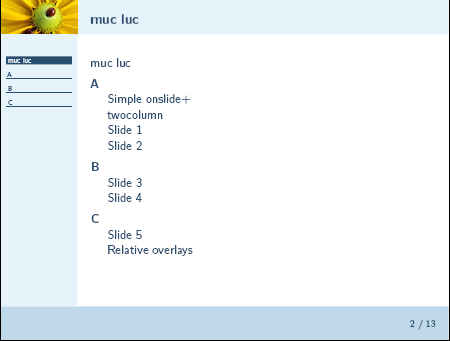
\includegraphics[trim=50 20 0 20,clip,%
    width=.17\slidewidth,height=.1\slideheight]{powerdot-default.ps}%
  }
}{
  \sbox\pd@imagebox{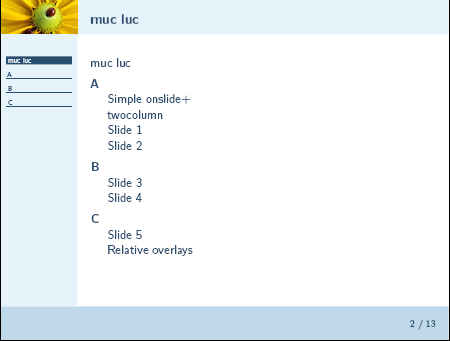
\includegraphics[trim=170 0 80 0,clip,%
    height=.1\slideheight]{powerdot-default.ps}%
  }
}
\pddefinetemplate{titleslide}{
  titlefont=\large\bfseries\centering,
  lfpos={.03\slidewidth,.04\slideheight},
  rfpos={.97\slidewidth,.04\slideheight},
  texthook=t,textpos={.5\slidewidth,.7\slideheight},
  textwidth=.9\slidewidth,textfont=\centering,
  textheight=.6\slideheight
}{%
  \psframe*[linecolor=pdllblue,linewidth=0pt]%
    (0,.8\slideheight)(\slidewidth,0)%
  \psline[linecolor=pddblue]%
    (0,.8\slideheight)(\slidewidth,.8\slideheight)%
}
\pddefinetemplate{basic}{
  titlepos={.2\slidewidth,.93\slideheight},
  titlewidth=.75\slidewidth,textheight=.68\slideheight,
  titlefont=\large\bfseries,
  lfpos={.03\slidewidth,.04\slideheight},
  rfpos={.97\slidewidth,.04\slideheight},
  tocitemsep=.6ex,
  toctcolor=pddblue,
  tochlcolor=pddblue,
  tochltcolor=pdllblue,
  sectionskip=.25\slideheight,sectionfont=\Large\bfseries\centering,
  ifsetup=portrait,
  textpos={.05\slidewidth,.83\slideheight},
  textwidth=.9\slidewidth,
  tocsecsep=.6ex,
  stochook=tr,stocpos={.48\slidewidth,.09\slideheight},
  stocfont=\tiny\raggedleft,
  ntochook=tl,ntocpos={.52\slidewidth,.09\slideheight},
  ntocfont=\tiny\raggedright,
  ifsetup=landscape,
  textpos={.2\slidewidth,.83\slideheight},
  textwidth=.75\slidewidth
}{%
  \psframe*[linecolor=pdllblue,linewidth=0pt]%
    (0,\slideheight)(\slidewidth,.9\slideheight)%
  \psframe*[linecolor=pdlblue,linewidth=0pt]%
    (0,0)(\slidewidth,.1\slideheight)%
  \rput[tl](0,\slideheight){\usebox\pd@imagebox}%
}
\pddefinetemplate[basic]{wideslide}{
  textpos={.05\slidewidth,.83\slideheight},
  textwidth=.9\slidewidth
}{}
\pddefinetemplate[basic]{slide}{
  ifsetup=landscape,
  tocpos={.015\slidewidth,.83\slideheight},
  tocwidth=.14\slidewidth,
  tocsecm={\psline[linewidth=.5pt,linecolor=pddblue]%
    (-.05,-.05)(.143\slidewidth,-.05)}
}{%
  \pdifsetup{landscape}{%
    \psframe[fillstyle=solid,fillcolor=pdllblue,linestyle=none,%
      linewidth=0pt](0,.9\slideheight)(.17\slidewidth,.1\slideheight)%
  }{}%
}
\setkeys[pd]{section}{widesectemp=wideslide}
\RequirePackage{pifont}
\def\labelitemi{\footnotesize\ding{110}}
\def\labelitemii{\small\ding{117}}
\def\labelitemiii{\tiny\ding{110}}
\def\labelitemiv{\tiny\ding{117}}
\pdsetup{
  list={labelsep=1em,leftmargin=*,itemsep=0pt,topsep=5pt,parsep=0pt}
}
\color{pddblue}
\def\rmdefault{cmss}
%</pddefault>
%
%<*pdtycja>
\NeedsTeXFormat{LaTeX2e}[1995/12/01]
\ProvidesPackage{powerdot-tycja}[2005/09/04 v1.0 tycja style (HA)]
\RequirePackage{pst-grad}
\definecolor{pdblue}{rgb}{.09,.27,.47}
\definecolor{pdyellow}{rgb}{1,.81,.42}
\definecolor{pdlyellow}{rgb}{1,.97,.84}
\pddefinetemplate{basic}{
  lfpos={.03\slidewidth,.04\slideheight},
  lffont=\scriptsize\color{pdlyellow},
  rfpos={.97\slidewidth,.04\slideheight},
  rffont=\scriptsize\color{pdlyellow},
  textheight=.68\slideheight,
  tocitemsep=.6ex,
  sectionskip=.25\slideheight,sectionfont=\centering\Large\bfseries,
  ifsetup=landscape,
  toctcolor=pdblue,
  tochlcolor=pdblue,
  tochltcolor=pdlyellow,
  tocpos={.845\slidewidth,.83\slideheight},
  tocwidth=.14\slidewidth,
  tocsecm={\psline[linewidth=.5pt,linecolor=pdblue]%
    (-.05,-.05)(.143\slidewidth,-.05)},
  ifsetup=portrait,
  toctcolor=pdlyellow,
  tochlcolor=pdlyellow,
  tochltcolor=pdblue,
  tocsecsep=.6ex,
  stochook=tr,stocpos={.48\slidewidth,.09\slideheight},
  stocfont=\tiny\raggedleft,
  ntochook=tl,ntocpos={.52\slidewidth,.09\slideheight},
  ntocfont=\tiny\raggedright
}{%
  \psframe*[linecolor=pdlyellow,linewidth=0pt]%
    (0,0)(\slidewidth,\slideheight)%
  \psframe*[linecolor=pdblue,linewidth=0pt]
    (0,0)(\slidewidth,.1\slideheight)%
  \psline[linecolor=pdblue]%
    (0,.87\slideheight)(.1\slidewidth,.87\slideheight)%
    (.1\slidewidth,.9\slideheight)(\slidewidth,.9\slideheight)%
}
\pddefinetemplate[basic]{titleslide}{
  titlefont=\large\bfseries\centering,texthook=t,
  textpos={.5\slidewidth,.7\slideheight},
  textwidth=.75\slidewidth,textfont=\centering,
  textheight=.55\slideheight,
  ifsetup=landscape,tocpos,ifsetup=portrait,stocpos,ntocpos
}{}
\pddefinetemplate[basic]{slide}{
  titlehook=Br,titlepos={.81\slidewidth,.93\slideheight},
  titlewidth=.76\slidewidth,titlefont=\large\bfseries\raggedleft,
  textpos={.12\slidewidth,.83\slideheight},textwidth=.67\slidewidth,
  ifsetup=portrait,
  titlepos={.9\slidewidth,.93\slideheight},titlewidth=.88\slidewidth,
  textwidth=.76\slidewidth
}{%
  \pdifsetup{landscape}{%
    \psframe[linestyle=none,fillstyle=gradient,gradbegin=pdyellow,%
      gradend=pdlyellow,gradmidpoint=1,linewidth=0pt]%
      (\slidewidth,.1\slideheight)(.83\slidewidth,\slideheight)%
  }{%
    \psframe[linestyle=none,fillstyle=gradient,gradbegin=pdyellow,%
      gradend=pdlyellow,gradmidpoint=1,linewidth=0pt]%
      (\slidewidth,.1\slideheight)(.92\slidewidth,\slideheight)%
  }%
}
\pddefinetemplate[basic]{wideslide}{
  titlehook=Br,titlepos={.81\slidewidth,.93\slideheight},
  titlewidth=.76\slidewidth,titlefont=\large\bfseries\raggedleft,
  textpos={.12\slidewidth,.83\slideheight},textwidth=.84\slidewidth,
  ifsetup=landscape,tocpos,ifsetup=portrait,
  titlepos={.9\slidewidth,.93\slideheight},titlewidth=.88\slidewidth,
}{%
  \pdifsetup{landscape}{%
    \psframe[linestyle=none,fillstyle=gradient,gradbegin=pdyellow,%
      gradend=pdlyellow,gradmidpoint=1,linewidth=0pt]%
      (\slidewidth,.1\slideheight)(.83\slidewidth,\slideheight)%
    \psframe*[linecolor=pdlyellow,linewidth=0pt]%
      (.79\slidewidth,.9\slideheight)(\slidewidth,.1\slideheight)%
  }{%
    \psframe[linestyle=none,fillstyle=gradient,gradbegin=pdyellow,%
      gradend=pdlyellow,gradmidpoint=1,linewidth=0pt]%
      (\slidewidth,.1\slideheight)(.92\slidewidth,\slideheight)%
    \psframe*[linecolor=pdlyellow,linewidth=0pt]%
      (.9\slidewidth,.9\slideheight)(\slidewidth,.1\slideheight)%
  }%
  \psline[linecolor=pdblue]%
    (0,.87\slideheight)(.1\slidewidth,.87\slideheight)%
    (.1\slidewidth,.9\slideheight)(\slidewidth,.9\slideheight)%
}
\setkeys[pd]{section}{widesectemp=wideslide}
\RequirePackage{pifont}
\def\labelitemi{\footnotesize\ding{110}}
\def\labelitemii{\small\ding{117}}
\def\labelitemiii{\tiny\ding{110}}
\def\labelitemiv{\tiny\ding{117}}
\pdsetup{
  list={labelsep=1em,leftmargin=*,itemsep=0pt,topsep=5pt,parsep=0pt}
}
\color{pdblue}
\def\rmdefault{cmss}
%</pdtycja>
%
%<*pdikeda>
\NeedsTeXFormat{LaTeX2e}[1995/12/01]
\ProvidesPackage{powerdot-ikeda}[2005/09/04 v1.0 ikeda style (CE,HA)]
\RequirePackage{calc}
\definecolor{pdplum}{rgb}{.435,.031,.165}
\definecolor{pddarkblue}{rgb}{.051,.094,.29}
\definecolor{pdgogreen}{rgb}{.051,.329,.29}
\definecolor{pdoffwhite}{rgb}{.941,.98,1}
\pddefinetemplate{titleslide}{
  titlefont=\Large\bfseries\centering,
  texthook=tl,
  textpos={.13\slidewidth,.7\slideheight},
  textwidth=.75\slidewidth,
  textfont=\centering,
  textheight=.56\slideheight
}{%
  \psframe[linestyle=none,fillstyle=solid,linewidth=0pt,%
    fillcolor=pdplum](0,\slideheight)(\slidewidth,0)%
  \psframe[linestyle=none,fillstyle=solid,fillcolor=pddarkblue]%
    (.05\slidewidth,.95\slideheight)(.95\slidewidth,.05\slideheight)%
  \psline[linestyle=solid,linecolor=pdoffwhite,linewidth=.01]%
    (.1\slidewidth,.1\slideheight)(.1\slidewidth,.9\slideheight)%
  \psline[linestyle=solid,linecolor=pdoffwhite,linewidth=.01]%
    (.9\slidewidth,.1\slideheight)(.9\slidewidth,.9\slideheight)%
  \pspolygon[linestyle=none,framearc=.3,fillstyle=vlines*,fillcolor=pdplum,%
    hatchcolor=pdoffwhite,hatchwidth=.1\pslinewidth,hatchsep=.005\linewidth]%
    (.1\slidewidth,.1\slideheight)(.25\slidewidth,.07\slideheight)%
    (.5\slidewidth,.1\slideheight)(.75\slidewidth,.13\slideheight)%
    (.9\slidewidth,.1\slideheight)%
  \pspolygon[linestyle=none,framearc=.3,fillstyle=hlines*,fillcolor=pdplum,%
    hatchcolor=pdoffwhite,hatchwidth=.1\pslinewidth,hatchsep=.005\linewidth]%
    (.1\slidewidth,.9\slideheight)(.25\slidewidth,.93\slideheight)%
    (.5\slidewidth,.9\slideheight)(.75\slidewidth,.87\slideheight)%
    (.9\slidewidth,.9\slideheight)%
}
\pddefinetemplate{basic}{
  titlewidth=.75\slidewidth,
  titlehook=Bl,
  titlefont=\large\bfseries\centering,
  sectionfont=\large\bfseries\centering,
  lfpos={.19\slidewidth,.025\slideheight},
  rfpos={.97\slidewidth,.025\slideheight},
  ifsetup=portrait,
  textpos={.05\slidewidth,.83\slideheight},
  textwidth=.9\slidewidth,
  ifsetup=landscape,
  textpos={.2\slidewidth,.84\slideheight},
  textwidth=.75\slidewidth
}{%
  \psframe*[linecolor=pddarkblue,linewidth=0pt]%
    (0,0)(\slidewidth,\slideheight)%
}
\pddefinetemplate[basic]{slide}{
  tocitemsep=.6ex,
  toctcolor=pdoffwhite,
  tochlcolor=pddarkblue,
  tochltcolor=pdoffwhite,
  ifsetup=landscape,
  titlepos={.2\slidewidth,.92\slideheight},
  tocpos={.01\slidewidth,.83\slideheight},
  tocwidth=.14\slidewidth,
  tocsecm={\psline[linewidth=.5pt,linecolor=pddarkblue](-.05,-.05)(.143\slidewidth,-.05)},
  sectionskip=.5in,
  textheight=.72\slideheight,
  ifsetup=portrait,
  titlepos={.02\slidewidth,.88\slideheight},
  titlewidth=.95\slidewidth,
  textheight=.64\slideheight,
  lfpos={.03\slidewidth,.025\slideheight},
  rfpos={.97\slidewidth,.025\slideheight},
  tocsecsep=.6ex,
  stochook=tr,stocpos={.47\slidewidth,.15\slideheight},
  stocfont=\tiny\raggedleft,
  ntochook=tl,ntocpos={.53\slidewidth,.15\slideheight},
  ntocfont=\tiny\raggedright
}{{%
  \psset{linestyle=none}%
  \pdifsetup{landscape}{%
    \psframe[fillstyle=solid,fillcolor=pdplum,linewidth=0pt]%
      (0,0)(.16\slidewidth,\slideheight)%
    \setlength\@tempdima{.16\slidewidth-.4cm}%
    \setlength\@tempdimb{.97\slideheight-.8cm}%
    \psframe[fillstyle=solid,fillcolor=pddarkblue,linewidth=0pt]%
      (.16\slidewidth,.97\slideheight)(\@tempdima,\@tempdimb)%
    \setlength\@tempdima{.16\slidewidth+.4cm}%
    \psframe[fillstyle=solid,fillcolor=pdplum,linewidth=0pt]%
      (.16\slidewidth,.97\slideheight)(\@tempdima,\@tempdimb)%
    \pspolygon[framearc=.3,fillstyle=solid,fillcolor=pddarkblue]%
      (0,.935\slideheight)(.02\slidewidth,.945\slideheight)%
      (.065\slidewidth,.935\slideheight)(.11\slidewidth,.925\slideheight)%
      (.13\slidewidth,.935\slideheight)%
    \pspolygon[framearc=.3,fillstyle=hlines*,fillcolor=pdplum,%
      hatchcolor=pdoffwhite,hatchwidth=.1\pslinewidth,hatchsep=.005\linewidth]%
      (.185\slidewidth,.09\slideheight)(.335\slidewidth,.06\slideheight)%
      (.58\slidewidth,.09\slideheight)%
    \pspolygon[framearc=.3,fillstyle=vlines*,fillcolor=pdplum,%
      hatchcolor=pdoffwhite,hatchwidth=.1\pslinewidth,hatchsep=.005\linewidth]%
      (.58\slidewidth,.09\slideheight)(.825\slidewidth,.06\slideheight)%
      (.975\slidewidth,.09\slideheight)%
  }{%
    \pspolygon[framearc=.3,fillstyle=vlines*,fillcolor=pdplum,%
      hatchcolor=pdoffwhite,hatchwidth=.1\pslinewidth,hatchsep=.005\linewidth]%
      (.02\slidewidth,.95\slideheight)(.17\slidewidth,.98\slideheight)%
      (.5\slidewidth,.95\slideheight)%
    \pspolygon[framearc=.3,fillstyle=hlines*,fillcolor=pdplum,%
      hatchcolor=pdoffwhite,hatchwidth=0.1\pslinewidth,hatchsep=.005\linewidth]%
      (.5\slidewidth,.95\slideheight)(.82\slidewidth,.98\slideheight)%
      (.98\slidewidth,.95\slideheight)%
    \psframe[fillstyle=solid,fillcolor=pdplum,linewidth=0pt]%
      (0,0)(\slidewidth,.17\slideheight)%
    \pspolygon[framearc=.3,fillstyle=vlines*,fillcolor=pdplum,%
      hatchcolor=pddarkblue,hatchwidth=.1\pslinewidth,hatchsep=.002\linewidth]%
      (.05\slidewidth,.1\slideheight)(.08\slidewidth,.08\slideheight)%
      (.14\slidewidth,.1\slideheight)(.20\slidewidth,.12\slideheight)%
      (.23\slidewidth,.1\slideheight)%
    \pspolygon[framearc=.3,fillstyle=hlines*,fillcolor=pdplum,%
      hatchcolor=pddarkblue,hatchwidth=.1\pslinewidth,hatchsep=.002\linewidth]%
      (.77\slidewidth,.1\slideheight)(.80\slidewidth,.12\slideheight)%
      (.86\slidewidth,.1\slideheight)(.92\slidewidth,.08\slideheight)%
      (.95\slidewidth,.1\slideheight)%
  }%
}}
\pddefinetemplate[basic]{wideslide}{
  titlepos={.02\slidewidth,.88\slideheight},
  lfpos={.03\slidewidth,.025\slideheight},
  titlewidth=\slidewidth,
  texthook=tl,
  sectionskip=.5in,
  textpos={.025\slidewidth,.84\slideheight},
  textwidth=.95\slidewidth,
  textheight=.72\slideheight,
  ifsetup=portrait,
  titlewidth=.95\slidewidth,
  titlepos={.025\slidewidth,.92\slideheight},
  textpos={.025\slidewidth,.87\slideheight},
  textheight=.68\slideheight,
  tocitemsep=.6ex,
  toctcolor=pdoffwhite,
  tochlcolor=pddarkblue,
  tochltcolor=pdoffwhite,
  lfpos={.03\slidewidth,.025\slideheight},
  rfpos={.97\slidewidth,.025\slideheight},
  tocsecsep=.6ex,
  stochook=tr,stocpos={.47\slidewidth,.15\slideheight},
  stocfont=\tiny\raggedleft,
  ntochook=tl,ntocpos={.53\slidewidth,.15\slideheight},
  ntocfont=\tiny\raggedright
}{{%
  \psset{linestyle=none,framearc=.3}%
  \pdifsetup{landscape}{%
    \pspolygon[fillstyle=vlines*,fillcolor=pdplum,%
      hatchcolor=pdoffwhite,hatchwidth=.1\pslinewidth,hatchsep=.005\linewidth]%
      (.02\slidewidth,.95\slideheight)(.17\slidewidth,.98\slideheight)%
      (.5\slidewidth,.95\slideheight)%
    \pspolygon[fillstyle=hlines*,fillcolor=pdplum,%
      hatchcolor=pdoffwhite,hatchwidth=.1\pslinewidth,hatchsep=.005\linewidth]%
      (.5\slidewidth,.95\slideheight)(.83\slidewidth,.98\slideheight)%
      (.98\slidewidth,.95\slideheight)%
    \pspolygon[fillstyle=hlines*,fillcolor=pdplum,%
      hatchcolor=pdoffwhite,hatchwidth=.1\pslinewidth,hatchsep=.005\linewidth]%
      (.02\slidewidth,.09\slideheight)(.17\slidewidth,.06\slideheight)%
      (.5\slidewidth,.09\slideheight)%
    \pspolygon[fillstyle=vlines*,fillcolor=pdplum,%
      hatchcolor=pdoffwhite,hatchwidth=.1\pslinewidth,hatchsep=.005\linewidth]%
      (.5\slidewidth,.09\slideheight)(.83\slidewidth,.06\slideheight)%
      (.98\slidewidth,.09\slideheight)%
  }{%
    \psframe[fillstyle=solid,fillcolor=pdplum,framearc=0,%
      linewidth=0pt](0,0)(\slidewidth,.17\slideheight)%
    \pspolygon[fillstyle=vlines*,fillcolor=pdplum,%
      hatchcolor=pddarkblue,hatchwidth=.1\pslinewidth,hatchsep=.002\linewidth]%
      (.05\slidewidth,.1\slideheight)(.08\slidewidth,.08\slideheight)%
      (.14\slidewidth,.1\slideheight)(.2\slidewidth,.12\slideheight)%
      (.23\slidewidth,.1\slideheight)%
    \pspolygon[fillstyle=hlines*,fillcolor=pdplum,%
      hatchcolor=pddarkblue,hatchwidth=.1\pslinewidth,hatchsep=.002\linewidth]%
      (.77\slidewidth,.1\slideheight)(.8\slidewidth,.12\slideheight)%
      (.86\slidewidth,.1\slideheight)(.92\slidewidth,.08\slideheight)%
      (.95\slidewidth,.1\slideheight)%
  }%
}}
\setkeys[pd]{section}{widesectemp=wideslide}
\RequirePackage{pifont}
\def\labelitemi{\color{pdplum}\footnotesize\ding{110}}
\def\labelitemii{\color{pdgogreen}\small\ding{115}}
\def\labelitemiii{\color{pdplum}\tiny\ding{110}}
\def\labelitemiv{\color{pdgogreen}\tiny\ding{115}}
\pdsetup{
  list={labelsep=1em,leftmargin=*,itemsep=0pt,topsep=5pt,parsep=0pt}
}
\color{pdoffwhite}
\def\rmdefault{cmss}
%</pdikeda>
%
%<*pdfyma>
\NeedsTeXFormat{LaTeX2e}[1995/12/01]
\ProvidesPackage{powerdot-fyma}[2005/09/04 v1.0 fyma style (SA,HA)]
\definecolor{pddblue}{rgb}{.14,.34,.55}
\definecolor{pdblue}{rgb}{.24,.45,.7}
\definecolor{pdlblue}{rgb}{.88,.95,1}
\RequirePackage{pst-grad}
\pddefinetemplate{basic}{
  titlefont=\large\bfseries,
  tocitemsep=.6ex,
  toctcolor=pddblue,
  tochlcolor=pddblue,
  tochltcolor=red,
  sectionskip=.25\slideheight,
  sectionfont=\Large\bfseries\centering,
  ifsetup=portrait,
  textheight=.67\slideheight,
  titlepos={.06\slidewidth,.9\slideheight},
  titlewidth=.75\slidewidth,
  textpos={.09\slidewidth,.83\slideheight},
  textwidth=.85\slidewidth,
  tocsecsep=.6ex,
  stochook=tr,stocpos={.48\slidewidth,.12\slideheight},
  stocfont=\tiny\raggedleft,
  ntochook=tl,ntocpos={.52\slidewidth,.12\slideheight},
  lfpos={.06\slidewidth,.045\slideheight},
  rfpos={.94\slidewidth,.045\slideheight},
  ifsetup=landscape,
  titlepos={.205\slidewidth,.9\slideheight},
  titlewidth=.75\slidewidth,
  textheight=.72\slideheight,
  textpos={.23\slidewidth,.82\slideheight},
  textwidth=.72\slidewidth,
  lfpos={.04\slidewidth,.03\slideheight},
  rfpos={.96\slidewidth,.03\slideheight},
  tocpos={.04\slidewidth,.82\slideheight},
  tocwidth=.14\slidewidth,
  tocsecm={\psline[linewidth=.5pt,linecolor=pddblue]%
    (-.05,-.05)(.143\slidewidth,-.05)}
}{{%
  \psset{linewidth=.8pt,linecolor=pdblue}%
  \pdifsetup{landscape}{%
  \psframe[linestyle=none,fillstyle=gradient,gradbegin=pdlblue,%
    gradend=white,gradmidpoint=0,dimen=outer]%
    (.03\slidewidth,.97\slideheight)(.97\slidewidth,.055\slideheight)%
  \psline
    (.02\slidewidth,.055\slideheight)(.98\slidewidth,.055\slideheight)%
  \psline
    (.03\slidewidth,.07\slideheight)(.03\slidewidth,.045\slideheight)%
  \psline
    (.97\slidewidth,.07\slideheight)(.97\slidewidth,.045\slideheight)%
  }{%
  \psframe[linestyle=none,fillstyle=gradient,gradbegin=white,%
    gradend=pdlblue,gradmidpoint=.85,dimen=outer]%
    (.03\slidewidth,.97\slideheight)(.97\slidewidth,.03\slideheight)%
  \psline
    (.02\slidewidth,.03\slideheight)(.98\slidewidth,.03\slideheight)%
  \psline
    (.03\slidewidth,.045\slideheight)(.03\slidewidth,.02\slideheight)%
  \psline
    (.97\slidewidth,.045\slideheight)(.97\slidewidth,.02\slideheight)%
  }%
  \psline
    (.02\slidewidth,.97\slideheight)(.98\slidewidth,.97\slideheight)%
  \psline
    (.03\slidewidth,.98\slideheight)(.03\slidewidth,.955\slideheight)%
  \psline
    (.97\slidewidth,.98\slideheight)(.97\slidewidth,.955\slideheight)%
}}
\pddefinetemplate[basic]{titleslide}{
  texthook=t,textpos={.5\slidewidth,.7\slideheight},
  textwidth=.9\slidewidth,textfont=\centering,
  textheight=.6\slideheight,
  titlefont=\large\bfseries\centering,tocpos,ntocpos,stocpos
}{}
\pddefinetemplate[basic]{slide}{}{%
  \pdifsetup{landscape}{%
  \psframe[fillstyle=gradient,gradbegin=pdlblue,gradend=white,%
    gradmidpoint=1,linestyle=none,dimen=outer,linewidth=.8pt]%
    (.03\slidewidth,.97\slideheight)(.195\slidewidth,.055\slideheight)%
  }{}%
}
\pddefinetemplate[basic]{wideslide}{
  ifsetup=landscape,tocpos,
  titlepos={.055\slidewidth,.9\slideheight},
  titlewidth=.75\slidewidth,
  textpos={.07\slidewidth,.83\slideheight},
  textwidth=.83\slidewidth
}{}
\pddefinetemplate[slide]{sectionslide}{
  textwidth=.45\slidewidth,texthook=t,
  sectionskip=0pt,textheight=.25\slideheight,
  ifsetup=landscape,
  textpos={.59\slidewidth,.55\slideheight},
  ifsetup=portrait,
  textpos={.5\slidewidth,.55\slideheight}
}{{%
  \psset{linewidth=.8pt,linecolor=pdblue}%
  \pdifsetup{landscape}{%
  \psframe[fillstyle=solid,fillcolor=white,linestyle=none,dimen=outer]%
    (.34\slidewidth,.65\slideheight)(.84\slidewidth,.4\slideheight)%
  \psline
    (.33\slidewidth,.65\slideheight)(.85\slidewidth,.65\slideheight)%
  \psline
    (.33\slidewidth,.4\slideheight)(.85\slidewidth,.4\slideheight)%
  \psline
    (.34\slidewidth,.635\slideheight)(.34\slidewidth,.66\slideheight)%
  \psline
    (.34\slidewidth,.39\slideheight)(.34\slidewidth,.415\slideheight)%
  }{%
  \psframe[fillstyle=solid,fillcolor=white,linestyle=none,dimen=outer]%
    (.16\slidewidth,.65\slideheight)(.84\slidewidth,.4\slideheight)%
  \psline
    (.15\slidewidth,.65\slideheight)(.85\slidewidth,.65\slideheight)%
  \psline
    (.15\slidewidth,.4\slideheight)(.85\slidewidth,.4\slideheight)%
  \psline
    (.16\slidewidth,.635\slideheight)(.16\slidewidth,.66\slideheight)%
  \psline
    (.16\slidewidth,.39\slideheight)(.16\slidewidth,.415\slideheight)%
  }%
  \psline
    (.84\slidewidth,.635\slideheight)(.84\slidewidth,.66\slideheight)%
  \psline
    (.84\slidewidth,.39\slideheight)(.84\slidewidth,.415\slideheight)%
}}
\pddefinetemplate[wideslide]{sectionwideslide}{%
  textwidth=.45\slidewidth,texthook=t,
  sectionskip=0pt,textheight=.25\slideheight,
  textpos={.5\slidewidth,.55\slideheight}
}{{%
  \psset{linewidth=.8pt,linecolor=pdblue}%
  \psframe[fillstyle=solid,fillcolor=white,linestyle=none,dimen=outer]%
    (.16\slidewidth,.65\slideheight)(.84\slidewidth,.4\slideheight)%
  \psline
    (.15\slidewidth,.65\slideheight)(.85\slidewidth,.65\slideheight)%
  \psline
    (.15\slidewidth,.4\slideheight)(.85\slidewidth,.4\slideheight)%
  \psline
    (.16\slidewidth,.635\slideheight)(.16\slidewidth,.66\slideheight)%
  \psline
    (.16\slidewidth,.39\slideheight)(.16\slidewidth,.415\slideheight)%
  \psline
    (.84\slidewidth,.635\slideheight)(.84\slidewidth,.66\slideheight)%
  \psline
    (.84\slidewidth,.39\slideheight)(.84\slidewidth,.415\slideheight)%
}}
\setkeys[pd]{section}{
  sectemp=sectionslide,widesectemp=sectionwideslide
}
\def\pd@slidetitle#1{%
  \settowidth\@tempdima{#1}%
  \psline[linewidth=.8pt,linecolor=pddblue]%
    (0,-.15cm)(\@tempdima,-.15cm)#1%
}
\def\pd@tochighlight#1{%
  \begin{minipage}[b]\pd@@tocwidth
    \pd@usedtocfont\color\pd@@tochltcolor#1%
  \end{minipage}%
}
\pdifsetup{landscape}{\def\pd@tocentry#1{{\tiny\ensuremath\bullet} #1}}{}
\def\labelitemi{\small\ensuremath\bullet}
\def\labelitemii{\small\ensuremath\circ}
\def\labelitemiii{\scriptsize\ensuremath\bullet}
\def\labelitemiv{\scriptsize\ensuremath\circ}
\pdsetup{
  list={labelsep=1em,leftmargin=*,itemsep=0pt,topsep=5pt,parsep=0pt}
}
\color{pddblue}
\def\rmdefault{phv}
\def\sfdefault{phv}
\def\Hv@scale{.86}
%</pdfyma>
%
%<*pdsimple>
\NeedsTeXFormat{LaTeX2e}[1995/12/01]
\ProvidesPackage{powerdot-simple}[2005/09/04 v1.0 simple style (HA)]
\pddefinetemplate{titleslide}{
  titlefont=\large\bfseries\raggedright,
  lfpos={.03\slidewidth,.04\slideheight},
  rfpos={.97\slidewidth,.04\slideheight},
  texthook=tl,textpos={.05\slidewidth,.83\slideheight},
  textwidth=.9\slidewidth,textfont=\tabcolsep0pt,
  textheight=.66\slideheight
}{%
  \psline[linewidth=.8pt](0,.9\slideheight)(\slidewidth,.9\slideheight)%
  \psline[linewidth=.8pt](0,.1\slideheight)(\slidewidth,.1\slideheight)%
}
\pddefinetemplate{basic}{
  titlepos={.05\slidewidth,.93\slideheight},
  titlewidth=.9\slidewidth,textheight=.66\slideheight,
  titlefont=\large\bfseries,
  lfpos={.03\slidewidth,.04\slideheight},
  rfpos={.97\slidewidth,.04\slideheight},
  tocitemsep=.6ex,textheight=.68\slideheight,
  tochlcolor=gray,
  sectionskip=.25\slideheight,sectionfont=\Large\bfseries\centering,
  ifsetup=portrait,
  textpos={.05\slidewidth,.83\slideheight},
  textwidth=.9\slidewidth,
  tocsecsep=.6ex,
  stochook=tr,stocpos={.48\slidewidth,.09\slideheight},
  stocfont=\tiny\raggedleft,
  ntochook=tl,ntocpos={.52\slidewidth,.09\slideheight},
  ntocfont=\tiny\raggedright,
  ifsetup=landscape,
  textpos={.2\slidewidth,.83\slideheight},
  textwidth=.75\slidewidth
}{%
  \psline[linewidth=.8pt](0,.9\slideheight)(\slidewidth,.9\slideheight)%
  \psline[linewidth=.8pt](0,.1\slideheight)(\slidewidth,.1\slideheight)%
}
\pddefinetemplate[basic]{wideslide}{
  textpos={.05\slidewidth,.83\slideheight},
  textwidth=.9\slidewidth
}{}
\pddefinetemplate[basic]{slide}{
  ifsetup=landscape,
  tocpos={.015\slidewidth,.83\slideheight},
  tocwidth=.14\slidewidth,
  tocsecm={\psline[linewidth=.5pt,linecolor=gray]%
    (-.05,-.05)(.143\slidewidth,-.05)}
}{%
  \pdifsetup{landscape}{%
    \psframe[fillstyle=solid,fillcolor=black!10,linestyle=none,%
      linewidth=.8pt](-.01\slidewidth,.9\slideheight)%
      (.17\slidewidth,.1\slideheight)%
  }{}%
}
\setkeys[pd]{section}{widesectemp=wideslide}
\RequirePackage{amssymb,pifont}
\def\labelitemi{\footnotesize\ensuremath\square}
\def\labelitemii{\small--}
\def\labelitemiii{\tiny\ensuremath\triangleright}
\def\labelitemiv{\tiny\ding{110}}
\pdsetup{
  list={labelsep=1em,leftmargin=*,itemsep=0pt,topsep=5pt,parsep=0pt}
}
\color{black}
\def\rmdefault{cmss}
%</pdsimple>
%
%<*pdciment>
\NeedsTeXFormat{LaTeX2e}[1995/12/01]
\ProvidesPackage{powerdot-ciment}[2005/09/04 v1.0 default style (HA)]
\definecolor{pdred}{rgb}{.7,.1,.1}
\definecolor{pddgray}{rgb}{.2,.2,.2}
\definecolor{pdlgray}{rgb}{.75,.75,.75}
\pddefinetemplate{basic}{
  titlepos={.1\slidewidth,.93\slideheight},
  titlewidth=.85\slidewidth,
  titlefont=\color{pdred}\large\bfseries,
  lfpos={.05\slidewidth,.04\slideheight},
  lffont=\color{pddgray}\scriptsize,
  rffont=\color{pddgray}\scriptsize,
  rfpos={.95\slidewidth,.04\slideheight},
  tocitemsep=.6ex,
  toctcolor=black,
  tochlcolor=pdred,
  tochltcolor=white,
  sectionskip=.25\slideheight,
  sectionfont=\color{pdred}\Large\bfseries\centering,
  ifsetup=portrait,
  textpos={.05\slidewidth,.85\slideheight},
  textwidth=.9\slidewidth,textheight=.68\slideheight,
  tocsecsep=.6ex,
  stochook=tr,stocpos={.48\slidewidth,.13\slideheight},
  stocfont=\tiny\raggedleft,
  ntochook=tl,ntocpos={.52\slidewidth,.13\slideheight},
  ntocfont=\tiny\raggedright,
  ifsetup=landscape,
  textpos={.2\slidewidth,.85\slideheight},
  textwidth=.75\slidewidth,textheight=.7\slideheight
}{%
  \psframe[linewidth=0pt,linestyle=none,fillstyle=hlines,%
    hatchwidth=.4pt,hatchangle=0,hatchcolor=pdlgray]%
    (0,0)(\slidewidth,\slideheight)%
  \pdifsetup{landscape}{%
    \psline[linecolor=pdred](.05\slidewidth,.09\slideheight)%
      (.95\slidewidth,.09\slideheight)%
  }{%
    \psline[linecolor=pdred](.05\slidewidth,.15\slideheight)%
      (.95\slidewidth,.15\slideheight)%
  }%
}
\pddefinetemplate[basic]{titleslide}{
  titlefont=\color{pdred}\large\bfseries\centering,
  texthook=t,textpos={.5\slidewidth,.7\slideheight},
  textwidth=.9\slidewidth,textfont=\centering,
  textheight=.6\slideheight,titlepos,
  ifsetup=portrait,textheight=.53\slideheight
}{}
\pddefinetemplate[basic]{wideslide}{
  textpos={.05\slidewidth,.85\slideheight},
  textwidth=.9\slidewidth
}{}
\pddefinetemplate[basic]{slide}{
  ifsetup=landscape,
  tocpos={.015\slidewidth,.83\slideheight},
  tocwidth=.14\slidewidth,
  tocsecm={\psline[linewidth=.5pt,linecolor=pdred]%
    (-.05,-.05)(.143\slidewidth,-.05)}
}{%
  \pdifsetup{landscape}{%
    \psframe[fillstyle=solid,fillcolor=pdlgray,linestyle=none,%
      linewidth=0pt](0,.85\slideheight)(.17\slidewidth,.15\slideheight)%
  }{}%
}
\def\pd@slidetitle#1{%
  \psline[linecolor=pdred](0,-.15cm)(.85\slidewidth,-.15cm)%
  \settowidth\@tempdima{#1}%
  \psline[linecolor=pdred,linewidth=2.5pt]%
    (0,-.15cm)(\@tempdima,-.15cm)#1%
}
\pddefinetemplate[slide]{sectionslide}{titlepos}{}
\pddefinetemplate[wideslide]{sectionwideslide}{titlepos}{}
\setkeys[pd]{section}{sectemp=sectionslide,widesectemp=sectionwideslide}
\RequirePackage{pifont}
\pdifsetup{landscape}{\def\pd@tocentry#1{{\tiny\ding{226}}#1}}{}
\def\labelitemi{\footnotesize\ding{110}}
\def\labelitemii{\small\ding{117}}
\def\labelitemiii{\tiny\ding{110}}
\def\labelitemiv{\tiny\ding{117}}
\pdsetup{
  list={labelsep=1em,leftmargin=*,itemsep=0pt,topsep=5pt,parsep=0pt}
}
\color{black}
\def\rmdefault{cmss}
%</pdciment>
%
%<*pdstyletest>
%%
%% For testing, enter your style below.
%% Switch on only one paper/orient option at a time.
\documentclass[
  style=your style,
  paper=screen,
%%  paper=a4paper,
%%  paper=letterpaper,
  orient=landscape,
%%  orient=portrait,
  size=11,
%%  hlsections
]{powerdot}

\pdsetup{
  lf=left footer,
  rf=right footer
}

%% For testing text height.
\makeatletter
\def\textheightrule{%
  \raisebox\baselineskip{\rule{1cm}\pd@@textheight}%
}
\makeatother

\title{This is a test file to test new styles with --
this title is very long on purpose.\thanks{Adjust textheight
to position this footnote.}}
\author{Hendri Adriaens \and Christopher Ellison}
\date{August 16, 2005}

\begin{document}

\maketitle

\begin{slide}{Test normal slide}
  Lorem ipsum dolor sit amet, consectetuer adipiscing elit. Ut purus
  elit, vestibulum ut, placerat ac, adipiscing vitae, felis. Curabitur
  dictum gravida mauris. Nam arcu libero, nonummy eget, consectetuer
  id, vulputate a, magna. Donec vehicula augue eu neque. Pellentesque
  habitant morbi tristique senectus et netus et malesuada fames ac
  turpis egestas. Mauris ut leo. Cras viverra metus rhoncus sem.
\end{slide}

\begin{slide}{Test itemize}
  Some text.\pause
  \begin{itemize}
    \item level 1\pause
    \begin{itemize}
      \item level 2\pause
      \begin{itemize}
        \item level 3\pause
        \begin{itemize}
          \item level 4
        \end{itemize}
      \end{itemize}
    \end{itemize}
  \end{itemize}
  Some text.\footnote{Adjust textheight
  to position this footnote.}
\end{slide}

\section{Normal section}

\begin{slide}{Test enumerate and inactive color}
  Some text.\pause
  \begin{enumerate}[type=1]
    \item level 1\pause
    \begin{enumerate}
      \item level 2\pause
      \begin{enumerate}
        \item level 3\pause
        \begin{enumerate}
          \item level 4
        \end{enumerate}
      \end{enumerate}
    \end{enumerate}
  \end{enumerate}
  Some text.
\end{slide}

\begin{slide}{The rule has height \texttt{textheight}}
  \textheightrule
\end{slide}

\section[template=wideslide]{Wide slide section}

\begin{wideslide}{Test wideslide}
  Lorem ipsum dolor sit amet, consectetuer adipiscing elit. Ut purus
  elit, vestibulum ut, placerat ac, adipiscing vitae, felis. Curabitur
  dictum gravida mauris. Nam arcu libero, nonummy eget, consectetuer
  id, vulputate a, magna. Donec vehicula augue eu neque. Pellentesque
  habitant morbi tristique senectus et netus et malesuada fames ac
  turpis egestas. Mauris ut leo. Cras viverra metus rhoncus
  sem.\footnote{Adjust textheight to position this footnote.}
\end{wideslide}

\begin{wideslide}{The rule has height \texttt{textheight}}
  \textheightrule
\end{wideslide}

\end{document}
%</pdstyletest>
%
%<*pdexample1>
\documentclass{powerdot}

\title{powerdot example 1}
\author{Hendri Adriaens \and Christopher Ellison}

\begin{document}

\maketitle

\begin{slide}{Slide 1}
  \begin{itemize}
    \item This is the first slide\pause
    \item There is nothing special about it.
  \end{itemize}
\end{slide}

\section{First section}

\begin{slide}{Slide 2}
  \begin{itemize}
    \item<1-> Here
    \begin{itemize}
      \item<2-> we
      \begin{itemize}
        \item<3-> demonstrate
        \begin{itemize}
          \item<4-> the itemize environment
        \end{itemize}
      \end{itemize}
    \end{itemize}
  \end{itemize}
\end{slide}

\begin{slide}{Slide 3}
  \begin{enumerate}[type=1]
    \item<1> Here
    \begin{enumerate}
      \item<2> we
      \begin{enumerate}
        \item<3> demonstrate
        \begin{enumerate}
          \item<4> the enumerate environment
        \end{enumerate}
      \end{enumerate}
    \end{enumerate}
  \end{enumerate}
\end{slide}

\end{document}
%</pdexample1>
%
%<*pdexample2>
\documentclass[
  size=12,
  style=ikeda,
  paper=screen,
%% Try me!
%%  orient=portrait,
%%  mode=handout,
%%  display=slidesnotes,
  blackslide,
  nopagebreaks,
  fleqn
]{powerdot}

\title{powerdot example 2}
\author{Hendri Adriaens\and Christopher Ellison}

\pdsetup{
  lf=Example 2,
  rf=for powerdot,
  trans=Wipe,
  theslide=slide~\arabic{slide},
  list={itemsep=6pt}
}

\begin{document}

\maketitle

\begin{slide}{Slide 1}
  \begin{itemize}
    \item This is a bigger example\pause
    \item demonstrating more of the possibilities of powerdot.
  \end{itemize}
\end{slide}

\section{This section has a slide}

\begin{slide}{Slide 2}
  Here is the binomium formula.\pause
  \begin{equation}\label{binomium}
    (a+b)^n=\sum_{k=0}^n{n\choose k}a^{n-k}b^k
  \end{equation}\pause
  We will prove formula (\ref{binomium}) on the blackboard.\\
  \hyperlink{blackslide}{Click here to switch to the black slide.}
\end{slide}

\begin{note}{Note to slide 2}
  Here we could type the proof that
  we want to copy to the blackboard.
\end{note}

\begin{slide}{Slide 3}
  \begin{itemize}[type=1]
    \item This happens\dots\pause
    \item when you change\dots\pause
    \item the type of itemize.
  \end{itemize}
\end{slide}

\section[template=wideslide,tocsection=hidden]{A hidden wide section}

\begin{slide}{Slide 4}
  \begin{itemize}
    \item We only treat this material\dots\pause
    \begin{itemize}
      \item if we have some time left.\pause
      \item But don't hesitate\dots\pause
    \end{itemize}
    \item to read it yourself.
  \end{itemize}
\end{slide}

\begin{wideslide}{Slide 5}
  This wide slide can contain more material
  as it is wider and does not have a table
  of contents.
\end{wideslide}

\end{document}
%</pdexample2>
%
%<*preamble>
\usepackage{url}
%\usepackage{fourier}
\usepackage{xcolor}
\usepackage{enumitem}
\usepackage{pst-char}
\usepackage{listings}
\usepackage{array}
\usepackage{xkeyval}
\lstnewenvironment{command}{%
  \lstset{columns=flexible,frame=single,backgroundcolor=\color{white!20},%
    xleftmargin=\fboxsep,xrightmargin=\fboxsep,escapeinside=`',gobble=1}}{}
\lstnewenvironment{example}[1][]{%
  \lstset{basicstyle=\footnotesize\ttfamily,columns=flexible,frame=single,%
    backgroundcolor=\color{white!20},xleftmargin=\fboxsep,%
    xrightmargin=\fboxsep,gobble=1,%
%    language=[LaTeX]TeX,keywordstyle=\color{black},%
%    moretexcs=[1]{color,ProvidesPackage},%
%    moretexcs=[2]{onslide,pause,pdsetup,maketitle,tableofcontents},%
%    texcsstyle=[2]\color{white}%
    }\lstset{#1}}{}
\def\option#1{\fcolorbox{black}{red!20}{\texttt{#1}}\vspace*{.2cm}}
\def\mktitledecor{%
  \rput[tl]{90}(-5.5,-25.51){%
    \psline[linewidth=1pt](0,1.5)(\paperheight,1.5)%
    \rput[lB](.075\paperheight,.5){\pscharpath[linecolor=blue!50,%
      fillcolor=yellow!20,fillstyle=solid,linewidth=.5pt]%
      {\Huge\bfseries\sffamily powerdot}%
    }%
    \rput[rB](.925\paperheight,.5){\pscharpath[linecolor=blue!50,%
      fillcolor=yellow!20,fillstyle=solid,linewidth=.5pt]%
      {\Huge\bfseries Documentation}%
    }%
    \psline[linewidth=1pt](0,0)(\paperheight,0)%
  }%
}
\makeatletter
\def\tableofcontents{\@starttoc{toc}}
\renewenvironment{theglossary}{%
  \section*{Version history}%
  \GlossaryParms \let\item\@idxitem \ignorespaces
}{}%
\def\DescribeMacros{\leavevmode\@bsphack
  \begingroup\MakePrivateLetters\Describe@Macros}
\def\Describe@Macros#1{\endgroup\strut
  \marginpar{\raggedleft
  \def\@tempa{#1}\count@\z@
  \XKV@for@o\@tempa\@tempa{%
    \ifnum\count@>\z@\\\fi\advance\count@\@ne
    \MacroFont\expandafter\string\@tempa
    \expandafter\SpecialUsageIndex\expandafter{\@tempa}%
  }}%
  \@esphack\ignorespaces
}
\def\DescribeOption#1{\leavevmode\@bsphack
              \marginpar{\raggedleft\PrintDescribeOption{#1}}%
              \SpecialOptionIndex{#1}\@esphack\ignorespaces}
\def\PrintDescribeOption#1{\strut\emph{option}\\\MacroFont #1\ }
\def\SpecialOptionIndex#1{\@bsphack
    \index{#1\actualchar{\protect\ttfamily#1}
           (option)\encapchar usage}\@esphack}
\def\DescribeOptions#1{\leavevmode\@bsphack
  \marginpar{\raggedleft\strut\emph{options}%
  \@for\@tempa:=#1\do{%
    \\\strut\MacroFont\@tempa\SpecialOptionIndex\@tempa
  }}\@esphack\ignorespaces}
\def\SpecialEnvIndex#1{\@bsphack
    \index{#1\actualchar{\protect\ttfamily#1}
           (environment)\encapchar usage}\@esphack}
\def\changes@#1#2#3{%
  \protected@edef\@tempa{%
    \noexpand\glossary{\textbf{#1}\hfill\emph{(#2)}%
    \levelchar
    \ifx\saved@macroname\@empty
      \space\actualchar\generalname
    \else
      \expandafter\@gobble\saved@macroname
      \actualchar\string\verb\quotechar*%
      \verbatimchar\saved@macroname\verbatimchar
    \fi
    :\levelchar #3}%
  }%
  \@tempa\endgroup\@esphack
}
\makeatother
\def\PrintChangesX{%
  \begingroup
    \let\efill\relax
    \PrintChanges
  \endgroup
}
\def\PrintIndexX{%
  \begingroup
    \setcounter{IndexColumns}{2}
    \setlength{\columnsep}{18pt}%
    \setlength{\columnseprule}{.4pt}%
    \PrintIndex
  \endgroup
}
\def\larg#1{{\ttfamily\char`\<}\meta{#1}{\ttfamily\char`\>}}
\let\pf\textsf
\newcolumntype{d}{c|l}
\newcolumntype{e}{c|c|c|c}
\RecordChanges
\CodelineIndex
\newcounter{FAQ}
\def\question{%
  \stepcounter{FAQ}%
  \parskip4pt plus 2pt minus 1pt
  \itemsep4pt plus 2pt minus 1pt
  \parsep4pt plus 2pt minus 1pt
  \item[\textbf{Q\arabic{FAQ}}]%
}
\def\answer{%
  \parskip0pt
  \itemsep0pt
  \parsep0pt
  \item[\textbf{A\arabic{FAQ}}]%
}
%</preamble>
%
%<*bib>
@BOOK{companion,
  author       = {Frank Mittelbach and Michel Goossens and Johannes Braams and David Carlisle and Chris Rowley},
  title        = {The {\LaTeX} {C}ompanion, {S}econd {E}dition},
  year         = {2004},
  publisher    = {{Addison-Wesley}}
}

@MISC{PSTricks,
  author       = {{Timothy Van} {Zandt et al.}},
  title        = {\pf{PSTricks} package, v1.07, 2005/05/06},
  howpublished = {\url{CTAN:/graphics/pstricks}}
}

@MISC{PSTricksWeb,
  author       = {Herbert Vo\ss},
  title        = {\pf{PSTricks} website},
  howpublished = {\url{http://pstricks.tug.org}}
}

@MISC{xkeyval,
  author       = {Hendri Adriaens},
  title        = {\pf{xkeyval} package},
  howpublished = {\url{CTAN:/macros/latex/contrib/xkeyval}}
}

@MISC{extsizes,
  author       = {James Kilfiger and Wolfgang May},
  title        = {\pf{extsizes} bundle},
  howpublished = {\url{CTAN:/macros/latex/contrib/extsizes}}
}

@MISC{prosper,
  author       = {Fr\'ed\'eric Goualard and Peter M\o ller Neergaard},
  title        = {\pf{prosper} class},
  howpublished = {\url{CTAN:/macros/latex/contrib/prosper}}
}

@MISC{HA-prosper,
  author       = {Hendri Adriaens},
  title        = {\pf{HA-prosper} package},
  howpublished = {\url{CTAN:/macros/latex/contrib/HA-prosper}}
}

@MISC{enumitem,
  author       = {Javier Bezos},
  title        = {\pf{enumitem} package},
  howpublished = {\url{CTAN:/macros/latex/contrib/enumitem}}
}

@MISC{hyperref,
  author       = {Sebastian Rahtz and Heiko Overdiek},
  title        = {\pf{hyperref} package},
  howpublished = {\url{CTAN:/macros/latex/contrib/hyperref}}
}

@MISC{natbib,
  author       = {Patrick W. Daly},
  title        = {\pf{natbib} package},
  howpublished = {\url{CTAN:/macros/latex/contrib/natbib}}
}

@MISC{geometry,
  author       = {Hideo Umeki},
  title        = {\pf{geometry} package},
  howpublished = {\url{CTAN:/macros/latex/contrib/geometry}}
}

@MISC{float,
  author       = {Anselm Lingnau},
  title        = {\pf{float} package},
  howpublished = {\url{CTAN:/macros/latex/contrib/float}}
}

@MISC{xcolor,
  author       = {Uwe Kern},
  title        = {\pf{xcolor} package},
  howpublished = {\url{CTAN:/macros/latex/contrib/xcolor}}
}

@MISC{graphics,
  author       = {David Carlisle},
  title        = {\pf{graphics} bundle},
  howpublished = {\url{CTAN:/macros/latex/required/graphics}}
}

@MISC{CTAN,
  author       = {CTAN crew},
  title        = {{The Comprehensive TeX Archive Network}},
  howpublished = {\url{http://www.ctan.org}}
}
%</bib>
